%  LaTeX support: latex@mdpi.com 
%  For support, please attach all files needed for compiling as well as the log file, and specify your operating system, LaTeX version, and LaTeX editor.


%=================================================================
\documentclass[agriculture,article,submit,pdftex,moreauthors]{Definitions/mdpi} 
%\documentclass[journal,article,submit,pdftex,moreauthors]{Definitions/mdpi} 


%\documentclass[preprints,article,submit,pdftex,moreauthors]{Definitions/mdpi} 
% For posting an early version of this manuscript as a preprint, you may use "preprints" as the journal. Changing "submit" to "accept" before posting will remove line numbers.

% Below journals will use APA reference format:
% admsci, behavsci, businesses, econometrics, economies, education, ejihpe, games, humans, ijfs, journalmedia, jrfm, languages, psycholint, publications, tourismhosp, youth

% Below journals will use Chicago reference format:
% arts, genealogy, histories, humanities, jintelligence, laws, literature, religions, risks, socsci

%--------------------
% Class Options:
%--------------------
%----------
% journal
%----------
% Choose between the following MDPI journals:
% accountaudit, acoustics, actuators, addictions, adhesives, admsci, adolescents, aerobiology, aerospace, agriculture, agriengineering, agrochemicals, agronomy, ai, air, algorithms, allergies, alloys, amh, analytica, analytics, anatomia, anesthres, animals, antibiotics, antibodies, antioxidants, applbiosci, appliedchem, appliedmath, appliedphys, applmech, applmicrobiol, applnano, applsci, aquacj, architecture, arm, arthropoda, arts, asc, asi, astronomy, atmosphere, atoms, audiolres, automation, axioms, bacteria, batteries, bdcc, behavsci, beverages, biochem, bioengineering, biologics, biology, biomass, biomechanics, biomed, biomedicines, biomedinformatics, biomimetics, biomolecules, biophysica, biosensors, biosphere, biotech, birds, blockchains, bloods, blsf, brainsci, breath, buildings, businesses, cancers, carbon, cardiogenetics, catalysts, cells, ceramics, challenges, chemengineering, chemistry, chemosensors, chemproc, children, chips, cimb, civileng, cleantechnol, climate, clinbioenerg, clinpract, clockssleep, cmd, cmtr, coasts, coatings, colloids, colorants, commodities, complications, compounds, computation, computers, condensedmatter, conservation, constrmater, cosmetics, covid, crops, cryo, cryptography, crystals, csmf, ctn, curroncol, cyber, dairy, data, ddc, dentistry, dermato, dermatopathology, designs, devices, diabetology, diagnostics, dietetics, digital, disabilities, diseases, diversity, dna, drones, dynamics, earth, ebj, ecm, ecologies, econometrics, economies, education, eesp, ejihpe, electricity, electrochem, electronicmat, electronics, encyclopedia, endocrines, energies, eng, engproc, ent, entomology, entropy, environments, epidemiologia, epigenomes, esa, est, famsci, fermentation, fibers, fintech, fire, fishes, fluids, foods, forecasting, forensicsci, forests, fossstud, foundations, fractalfract, fuels, future, futureinternet, futureparasites, futurepharmacol, futurephys, futuretransp, galaxies, games, gases, gastroent, gastrointestdisord, gastronomy, gels, genealogy, genes, geographies, geohazards, geomatics, geometry, geosciences, geotechnics, geriatrics, glacies, grasses, greenhealth, gucdd, hardware, hazardousmatters, healthcare, hearts, hemato, hematolrep, heritage, higheredu, highthroughput, histories, horticulturae, hospitals, humanities, humans, hydrobiology, hydrogen, hydrology, hygiene, idr, iic, ijerph, ijfs, ijgi, ijmd, ijms, ijns, ijpb, ijt, ijtm, ijtpp, ime, immuno, informatics, information, infrastructures, inorganics, insects, instruments, inventions, iot, j, jal, jcdd, jcm, jcp, jcs, jcto, jdad, jdb, jeta, jfb, jfmk, jimaging, jintelligence, jlpea, jmahp, jmmp, jmms, jmp, jmse, jne, jnt, jof, joitmc, joma, jop, jor, journalmedia, jox, jpbi, jpm, jrfm, jsan, jtaer, jvd, jzbg, kidney, kidneydial, kinasesphosphatases, knowledge, labmed, laboratories, land, languages, laws, life, lights, limnolrev, lipidology, liquids, literature, livers, logics, logistics, lubricants, lymphatics, machines, macromol, magnetism, magnetochemistry, make, marinedrugs, materials, materproc, mathematics, mca, measurements, medicina, medicines, medsci, membranes, merits, metabolites, metals, meteorology, methane, metrics, metrology, micro, microarrays, microbiolres, microelectronics, micromachines, microorganisms, microplastics, microwave, minerals, mining, mmphys, modelling, molbank, molecules, mps, msf, mti, multimedia, muscles, nanoenergyadv, nanomanufacturing, nanomaterials, ncrna, ndt, network, neuroglia, neurolint, neurosci, nitrogen, notspecified, nri, nursrep, nutraceuticals, nutrients, obesities, oceans, ohbm, onco, oncopathology, optics, oral, organics, organoids, osteology, oxygen, parasites, parasitologia, particles, pathogens, pathophysiology, pediatrrep, pets, pharmaceuticals, pharmaceutics, pharmacoepidemiology, pharmacy, philosophies, photochem, photonics, phycology, physchem, physics, physiologia, plants, plasma, platforms, pollutants, polymers, polysaccharides, populations, poultry, powders, preprints, proceedings, processes, prosthesis, proteomes, psf, psych, psychiatryint, psychoactives, psycholint, publications, purification, quantumrep, quaternary, qubs, radiation, reactions, realestate, receptors, recycling, regeneration, religions, remotesensing, reports, reprodmed, resources, rheumato, risks, robotics, rsee, ruminants, safety, sci, scipharm, sclerosis, seeds, sensors, separations, sexes, signals, sinusitis, siuj, skins, smartcities, sna, societies, socsci, software, soilsystems, solar, solids, spectroscj, sports, standards, stats, std, stresses, surfaces, surgeries, suschem, sustainability, symmetry, synbio, systems, tae, targets, taxonomy, technologies, telecom, test, textiles, thalassrep, therapeutics, thermo, timespace, tomography, tourismhosp, toxics, toxins, transplantology, transportation, traumacare, traumas, tropicalmed, universe, urbansci, uro, vaccines, vehicles, venereology, vetsci, vibration, virtualworlds, viruses, vision, waste, water, wem, wevj, wild, wind, women, world, youth, zoonoticdis

%---------
% article
%---------
% The default type of manuscript is "article", but can be replaced by: 
% abstract, addendum, article, benchmark, book, bookreview, briefcommunication, briefreport, casereport, changes, clinicopathologicalchallenge, comment, commentary, communication, conceptpaper, conferenceproceedings, correction, conferencereport, creative, datadescriptor, discussion, entry, expressionofconcern, extendedabstract, editorial, essay, erratum, fieldguide, hypothesis, interestingimages, letter, meetingreport, monograph, newbookreceived, obituary, opinion, proceedingpaper, projectreport, reply, retraction, review, perspective, protocol, shortnote, studyprotocol, supfile, systematicreview, technicalnote, viewpoint, guidelines, registeredreport, tutorial,  giantsinurology, urologyaroundtheworld
% supfile = supplementary materials

%----------
% submit
%----------
% The class option "submit" will be changed to "accept" by the Editorial Office when the paper is accepted. This will only make changes to the frontpage (e.g., the logo of the journal will get visible), the headings, and the copyright information. Also, line numbering will be removed. Journal info and pagination for accepted papers will also be assigned by the Editorial Office.

%------------------
% moreauthors
%------------------
% If there is only one author the class option oneauthor should be used. Otherwise use the class option moreauthors.

%---------
% pdftex
%---------
% The option pdftex is for use with pdfLaTeX. Remove "pdftex" for (1) compiling with LaTeX & dvi2pdf (if eps figures are used) or for (2) compiling with XeLaTeX.

%=================================================================
% MDPI internal commands - do not modify
\firstpage{1} 
\makeatletter 
\setcounter{page}{\@firstpage} 
\makeatother
\pubvolume{1}
\issuenum{1}
\articlenumber{0}
\pubyear{2025}
\copyrightyear{2024}
%\externaleditor{Firstname Lastname} % More than 1 editor, please add `` and '' before the last editor name
\datereceived{ } 
\daterevised{ } % Comment out if no revised date
\dateaccepted{ } 
\datepublished{ } 
%\datecorrected{} % For corrected papers: "Corrected: XXX" date in the original paper.
%\dateretracted{} % For retracted papers: "Retracted: XXX" date in the original paper.
\hreflink{https://doi.org/} % If needed use \linebreak
%\doinum{}
%\pdfoutput=1 % Uncommented for upload to arXiv.org
%\CorrStatement{yes}  % For updates
%\longauthorlist{yes} % For many authors that exceed the left citation part

%=================================================================
% Add packages and commands here. The following packages are loaded in our class file: fontenc, inputenc, calc, indentfirst, fancyhdr, graphicx, epstopdf, lastpage, ifthen, float, amsmath, amssymb, lineno, setspace, enumitem, mathpazo, booktabs, titlesec, etoolbox, tabto, xcolor, colortbl, soul, multirow, microtype, tikz, totcount, changepage, attrib, upgreek, array, tabularx, pbox, ragged2e, tocloft, marginnote, marginfix, enotez, amsthm, natbib, hyperref, cleveref, scrextend, url, geometry, newfloat, caption, draftwatermark, seqsplit
% cleveref: load \crefname definitions after \begin{document}

% BEM ADDITIONS BEGIN
\usepackage{longtable}
\usepackage{amsmath}

% BEM ADDITIONS END

%=================================================================
% Please use the following mathematics environments: Theorem, Lemma, Corollary, Proposition, Characterization, Property, Problem, Example, ExamplesandDefinitions, Hypothesis, Remark, Definition, Notation, Assumption
%% For proofs, please use the proof environment (the amsthm package is loaded by the MDPI class).

%=================================================================
% Full title of the paper (Capitalized)
\Title{Approaches to Segmentation of Crop Images}

% MDPI internal command: Title for citation in the left column
\TitleCitation{Approaches to Segmentation of Crop Images}

% Author Orchid ID: enter ID or remove command
\newcommand{\orcidauthorA}{0009-0002-3582-2576} % Add \orcidA{} behind the author's name
%\newcommand{\orcidauthorB}{0000-0000-0000-000X} % Add \orcidB{} behind the author's name

% Authors, for the paper (add full first names)
%\Author{Evan McGinnis $^{1,\dagger,\ddagger}$\orcidA{}, Firstname Lastname $^{2,\ddagger}$ and Firstname Lastname $^{2,}$*}
\Author{Brian E McGinnis $^{1,\dagger,\ddagger}$\orcidA{}}

%\longauthorlist{yes}

% MDPI internal command: Authors, for metadata in PDF
\AuthorNames{Brian E McGinnis}

% MDPI internal command: Authors, for citation in the left column, only choose below one of them according to the journal style
% If this is a Chicago style journal: Lastname, Firstname, Firstname Lastname, and Firstname Lastname.
% If this is a APA style journal: Lastname, F., Lastname, F., \& Lastname, F.
% If this is a ACS style journal: Lastname, F.; Lastname, F.; Lastname, F.
%\isAPAStyle{%
%       \AuthorCitation{McGinnis, E., Lastname, F., \& Lastname, F.}
%         }{%
%        \isChicagoStyle{%
%        \AuthorCitation{McGinnis, E, Firstname Lastname, and Firstname Lastname.}
%        }{
%        \AuthorCitation{McGinnis, E.; Lastname, F.; Lastname, F.}
%        }
%}

\isAPAStyle{%
       \AuthorCitation{McGinnis, B.}
         }{%
        \isChicagoStyle{%
        \AuthorCitation{McGinnis, B}
        }{
        \AuthorCitation{McGinnis, B.}
        }
}

% Affiliations / Addresses (Add [1] after \address if there is only one affiliation.)
\address{%
$^{1}$ \quad Affiliation 1; evanmc@arizona.edu\\
}
%$^{2}$ \quad Affiliation 2; e-mail@e-mail.com}

% Contact information of the corresponding author
\corres{Correspondence: evanmc@arizona.edu}

% Current address and/or shared authorship
\firstnote{Current address: University of Arizona, Tucson, AZ 85721.}  % Current address should not be the same as any items in the Affiliation section.
\secondnote{These authors contributed equally to this work.}
% The commands \thirdnote{} till \eighthnote{} are available for further notes

%\simplesumm{} % Simple summary

%\conference{} % An extended version of a conference paper

% Abstract (Do not insert blank lines, i.e. \\) 
\abstract{This paper presents an overview of image segmentation under field conditions with ambient lighting. Discussed are index-based techniques using visible light using the RGB color space (Triangular Greenness, Normalized Difference, Excess Green, Excess Red, Color of Vegetation Extraction, Excess Green - Excess Red, Normalize Green-Red Difference, Vegetative, Combined Index I and II, and Modified Excess Green), using color spaces other than RGB (CIELab, YCbCr, and YIQ), and classification-based where each pixel is classified using machine-learning techniques (Multi-layer Perceptron, Linear Discriminant Analysis, and Support Vector Machine), and of deep-learning techniques (U-net). While index-based approaches proved to be the most practical, as classification based approaches tended to require more computation resources than are typically available under field conditions, index-based approaches often had significant errors that should be taken into account when selecting an approach. The index with the highest overall error rate was NGRDI, with 11.65\% of pixels mis-identified. An approach using the YIQ color space achieved the lowest error rate, with 1.4\%.}

% Keywords
\keyword{segmentation; vegetation index; semantic segmentation} 

% The fields PACS, MSC, and JEL may be left empty or commented out if not applicable
%\PACS{J0101}
%\MSC{}
%\JEL{}

%%%%%%%%%%%%%%%%%%%%%%%%%%%%%%%%%%%%%%%%%%
% Only for the journal Diversity
%\LSID{\url{http://}}

%%%%%%%%%%%%%%%%%%%%%%%%%%%%%%%%%%%%%%%%%%
% Only for the journal Applied Sciences
%\featuredapplication{Authors are encouraged to provide a concise description of the specific application or a potential application of the work. This section is not mandatory.}
%%%%%%%%%%%%%%%%%%%%%%%%%%%%%%%%%%%%%%%%%%

%%%%%%%%%%%%%%%%%%%%%%%%%%%%%%%%%%%%%%%%%%
% Only for the journal Data
%\dataset{DOI number or link to the deposited data set if the data set is published separately. If the data set shall be published as a supplement to this paper, this field will be filled by the journal editors. In this case, please submit the data set as a supplement.}
%\datasetlicense{License under which the data set is made available (CC0, CC-BY, CC-BY-SA, CC-BY-NC, etc.)}

%%%%%%%%%%%%%%%%%%%%%%%%%%%%%%%%%%%%%%%%%%
% Only for the journal Toxins
%\keycontribution{The breakthroughs or highlights of the manuscript. Authors can write one or two sentences to describe the most important part of the paper.}

%%%%%%%%%%%%%%%%%%%%%%%%%%%%%%%%%%%%%%%%%%
% Only for the journal Encyclopedia
%\encyclopediadef{For entry manuscripts only: please provide a brief overview of the entry title instead of an abstract.}

%%%%%%%%%%%%%%%%%%%%%%%%%%%%%%%%%%%%%%%%%%
% Only for the journal Advances in Respiratory Medicine and Smart Cities
%\addhighlights{yes}
%\renewcommand{\addhighlights}{%

%\noindent This is an obligatory section in “Advances in Respiratory Medicine'' and ``Smart Cities”, whose goal is to increase the discoverability and readability of the article via search engines and other scholars. Highlights should not be a copy of the abstract, but a simple text allowing the reader to quickly and simplified find out what the article is about and what can be cited from it. Each of these parts should be devoted up to 2~bullet points.\vspace{3pt}\\
%\textbf{What are the main findings?}
% \begin{itemize}[labelsep=2.5mm,topsep=-3pt]
% \item First bullet.
% \item Second bullet.
% \end{itemize}\vspace{3pt}
%\textbf{What is the implication of the main finding?}
% \begin{itemize}[labelsep=2.5mm,topsep=-3pt]
% \item First bullet.
% \item Second bullet.
% \end{itemize}
%}

%%%%%%%%%%%%%%%%%%%%%%%%%%%%%%%%%%%%%%%%%%
\begin{document}

%%%%%%%%%%%%%%%%%%%%%%%%%%%%%%%%%%%%%%%%%%
%\setcounter{section}{-1} %% Remove this when starting to work on the template.
%\section{How to Use this Template}
%
%The template details the sections that can be used in a manuscript. Note that the order and names of article sections may differ from the requirements of the journal (e.g., the positioning of the Materials and Methods section). Please check the instructions on the authors' page of the journal to verify the correct order and names. For any questions, please contact the editorial office of the journal or support@mdpi.com. For LaTeX-related questions please contact latex@mdpi.com.%\endnote{This is an endnote.} % To use endnotes, please un-comment \printendnotes below (before References). Only journal Laws uses \footnote.

% The order of the section titles is different for some journals. Please refer to the "Instructions for Authors” on the journal homepage.

\section{Introduction}
Agricultural images of crops taken from an overhead perspective typically contain only two things: vegetation and ground. While other items may appear in the image such as irrigation equipment or debris, the vast majority of images taken from from a low elevation (two feet, perhaps) will have only vegetation.  Images taken for tasks such as navigation tend to often include other features -- most notably, the horizon -- as they are acquired more parallel to the ground. While there may be things on the ground that must be ignored (irrigation equipment, ground debris, rocks), the goal of image segmentation remains unchanged: plants are retained in the final image, and everything else discarded. This document will discuss this process considering only visible light data using four techniques: index-based (the vegetated pixels are exaggerated and isolated from the background), Non-RGB colorspace thresholding (images in colorspaces such as YIQ are processed), classification-based (the pixels are classified as vegetation or ground), and deep-learning.  Image segmentation is often a first step in image processing, as doing so reduces the information content of an image for subsequent processing.  For example, it provides little value in a vegetation treatment system to classify a pebble on the ground as such -- that information can be safely discarded as the first step in image processing. The subsequent processing may be positive, applying an enhancement or treatment to vegetation identified as crop, or negative, applying a chemical, mechanical, or directed energy (i.e., laser) treatment to eliminate vegetation identified as weeds. This document will treat image segmentation as a preprocessing step in an overall workflow.
 

%%%%%%%%%%%%%%%%%%%%%%%%%%%%%%%%%%%%%%%%%%
\section{Materials and Methods}
Images were taken at the University of Arizona's Maricopa Agricultural Center (MAC) located in Maricopa, AZ (N 33.061857, E 111.967145) of a cantaloupe planting in May 2024. Images were obtained using an Apple IPhone 8, using ambient lighting. These images were color corrected using values obtained from images taken under identical lighting conditions of a Datacolor Sypder correction chart.  Images obtained using other sources are used to illustrate techniques or points, but most of the analysis shown in this document are from the set gathered at the MAC. All processing software was written in Python 3 and data analysis written in R.  
%%%%%%%%%%%%%%%%%%%%%%%%%%%%%%%%%%%%%%%%%%
\section{Results}
Three techniques are examined in this paper: index-based, machine-learning, and deep-learning.

\subsection{Index Based}
Index-based approaches follow the same basic workflow: a mask is produced from the original image and then applied to that image, retaining vegetated pixels, while discarding non-vegetated pixels. Figure~\ref{fig:index-segmentation} demonstrates an example of applying this process. starting with an image acquired under field conditions. The resulting image can be subsequently processed with the knowledge that all remaining pixels in the image are plants.

\begin{figure}[H]
	\centering
	\subfloat[Field view]{\includegraphics[width=0.25\linewidth]{figures/original.jpg}\label{fig:field-view}}
	\hfill
	\subfloat[NDI Mask]{
\includegraphics[width=0.25\linewidth]{figures/original-mask.jpg}\label{fig:index-mask}} 
	\hfill
	\subfloat[Masked Image]{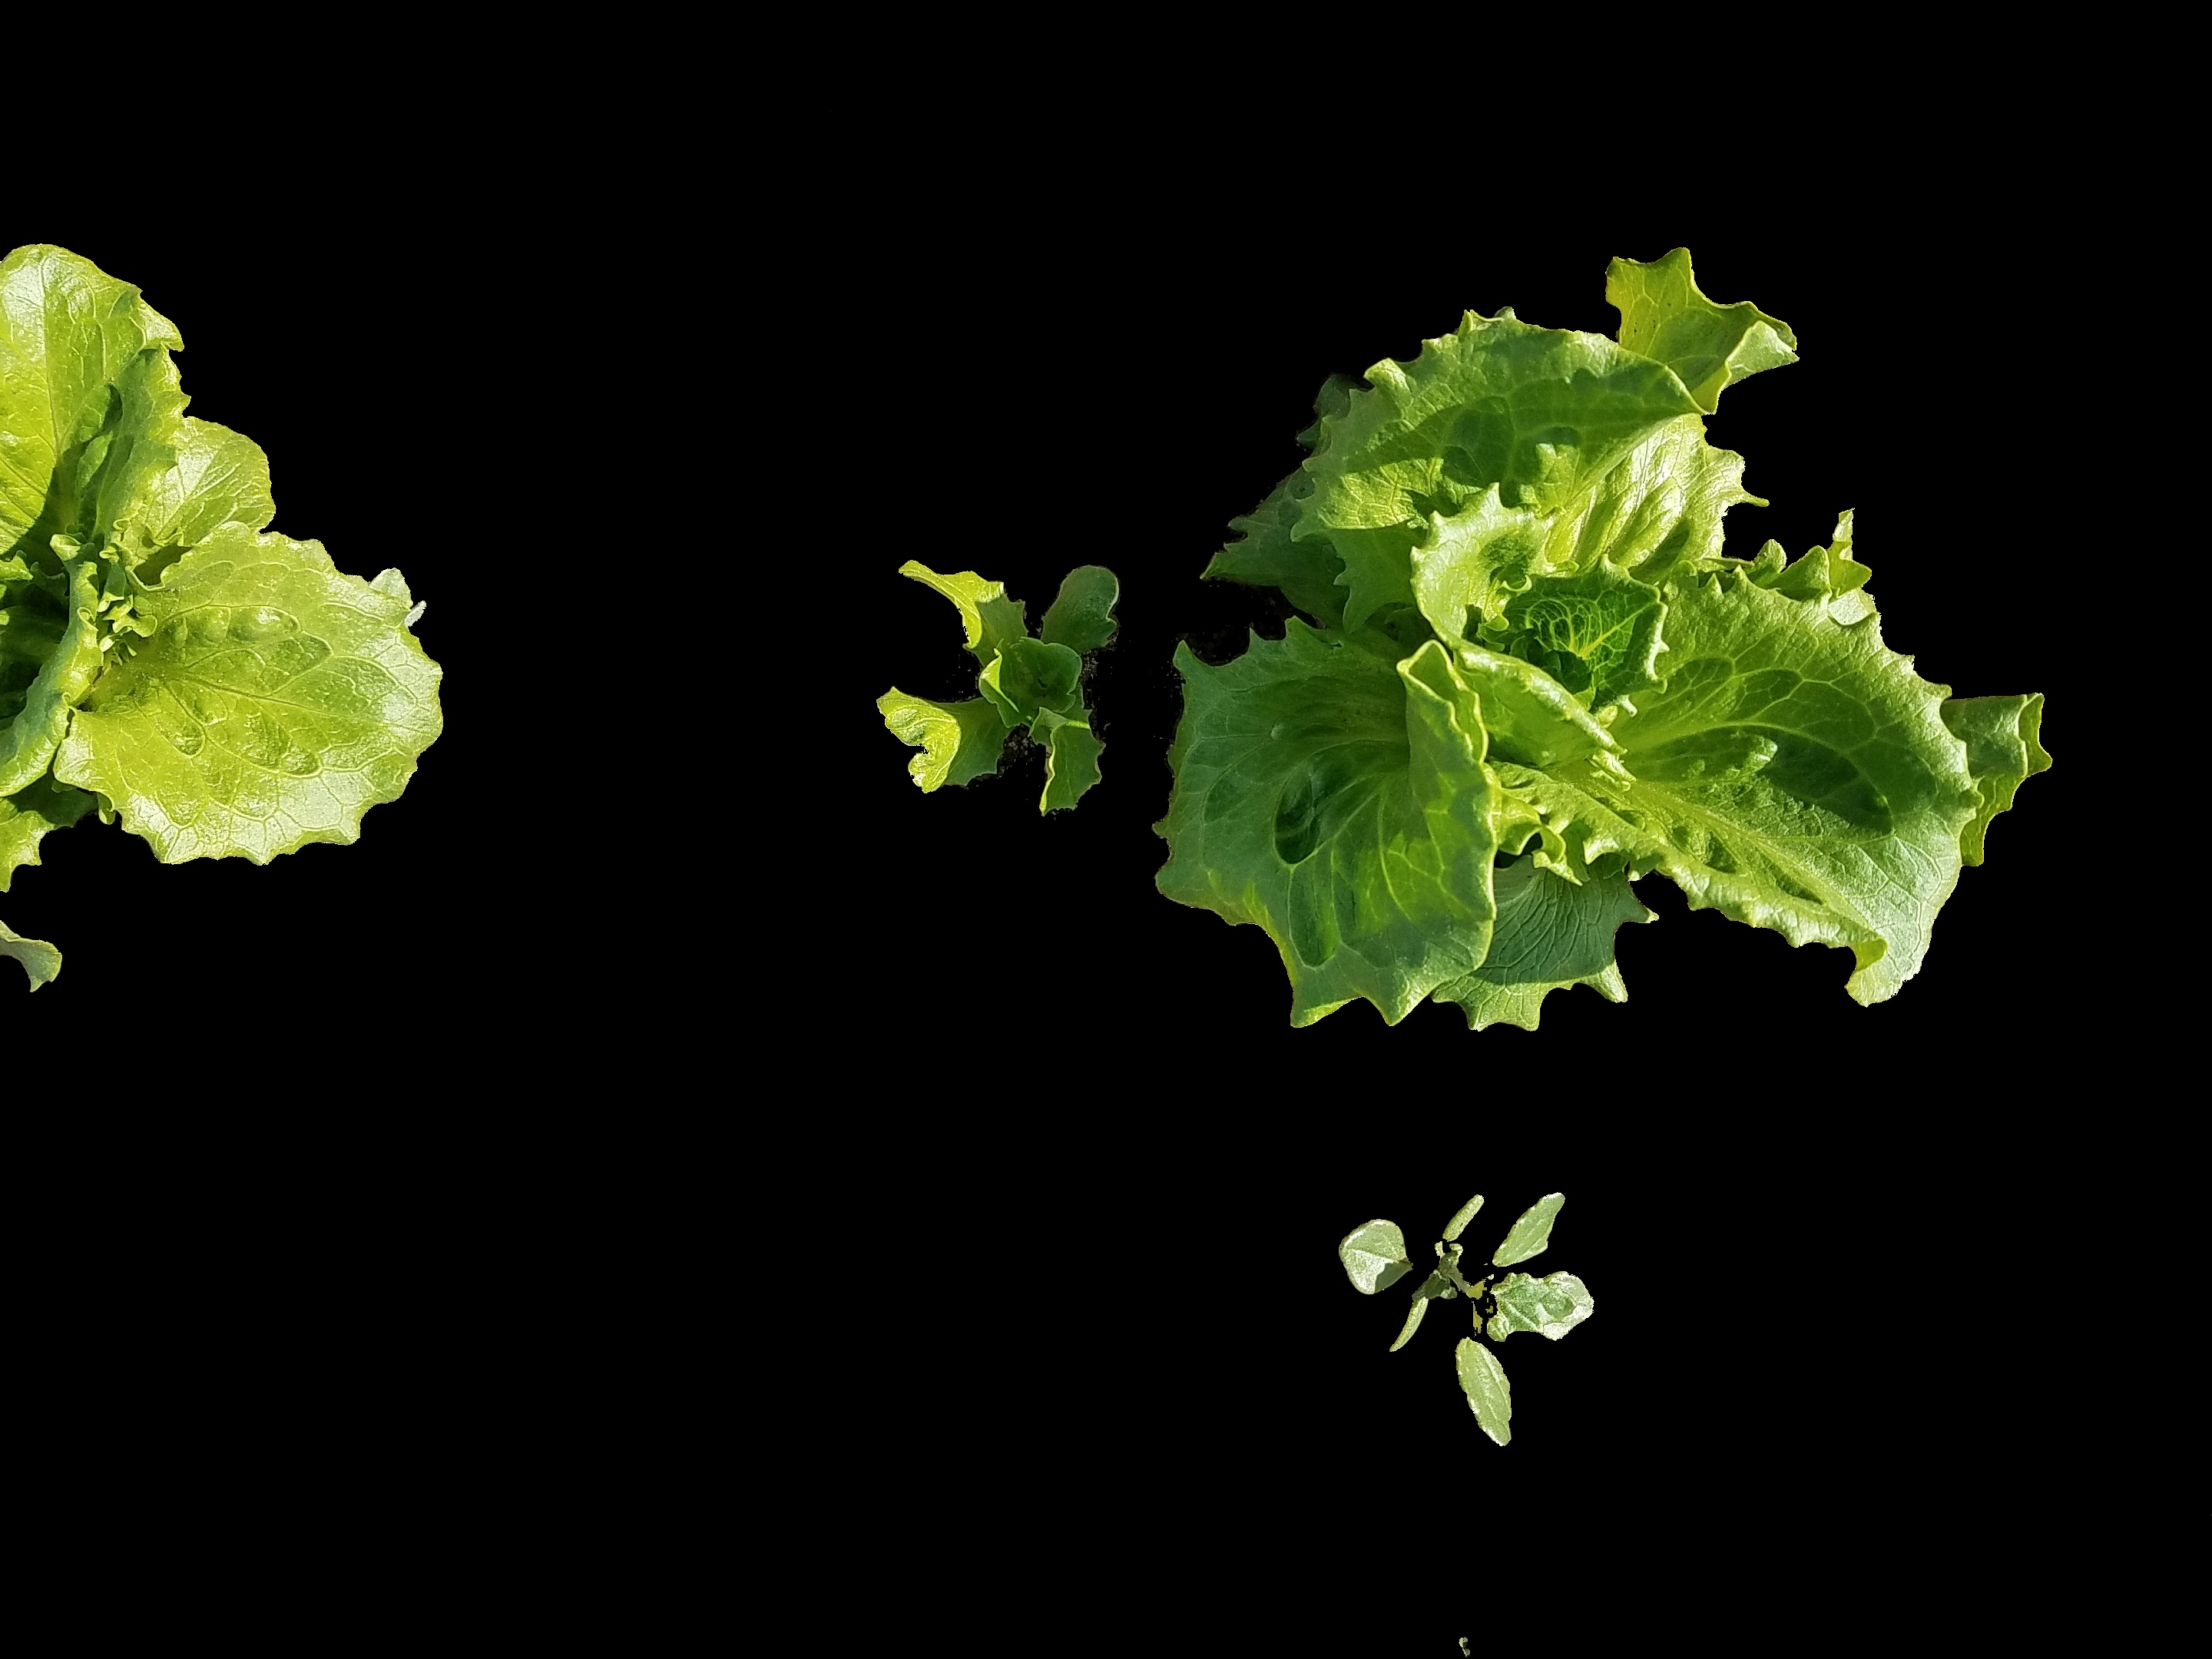
\includegraphics[width=0.25\linewidth]{figures/original-masked.jpg}\label{fig:original-masked-index}}
	\caption[Before and after segmentation]{Before and after segmentation. Note the absence of the stems seen in the weed in the lower portion of~\ref{fig:original-masked-index} -- this is made a bit more obvious with a close examination of the mask shown in \ref{fig:index-mask}.  This is an example of one of the shortcomings of some of the index based approaches that will be discussed in Section~\ref{section:problems-color}. The stems of the weed are not sufficiently green ``enough'' to register as vegetation.}
	\label{fig:index-segmentation}
\end{figure}

\subsubsection{RGB}
This commonly-encountered colorspace is often the only color space representation available from consumer cameras (dedicated or embedded within a phone), although machine vision cameras often can be configured to capture images in other spaces. This space is a fairly simple encoding of the amounts of Red, Green, and Blue of a pixel. A \textit{vegetation index} is used that exaggerates the pixel values typically associated with vegetation while minimizing non-vegetated pixel values.

These indices are used to create a mask that is then applied to the original source image to permit vegetation to show while masking details that are not relevant (ground pixels, stones, and other items that may appear in field conditions) The intent here is to remove all pixels that are not vegetated while leaving the vegetated pixels unmanipulated. The formulae for various RGB indices are shown in Table~\ref{table:indices}. References to specific bands (\textit{red} or \textit{R}, for instance) refer to the specific value that pixel has in that band.

\begin{table}[H]
\caption{Color Indices}
%\isPreprints{\centering} % If the paper is ``preprints'', please uncomment this parenthesis.
%\isPreprints{\begin{tabularx}{\textwidth}{CCCC}} % If the paper is ``preprints'', please uncomment this parenthesis.
			\toprule
			\textbf{Index}	& \textbf{Formula}	& \textbf{Abbreviation \& Reference}     \\
			\midrule
			\multirow[m]{1}{*}{Triangular Greenness}	
				& \begin{minipage}[t]{0.3\textwidth}
					$R_{green} - \alpha R_{red} - \beta R_{blue}\\ \alpha = \frac {2(\lambda_{blue} - \lambda_{green})} {(\lambda_{blue} - \lambda_{red})}\\ 
			    		\beta = \frac {2(\lambda_{green} - \lambda_{red})} {(\lambda_{blue} - \lambda_{red})} $
			   	\end{minipage}     
				& TGI - \cite{Hunt2013-ih}\\
			\addlinespace
                   %\midrule
			\multirow[m]{1}{*}{Normalized Difference}	
				& \begin{minipage}[t]{0.3\textwidth}
					$128 * \left( \left( \frac {(G - R)} {(G + R)} \right) + 1 \right)$
			   	\end{minipage}     
				& NDI - \cite{Woebbecke1995-bw}\\
			\addlinespace
                  %\midrule
			\multirow[m]{1}{*}{Excess Green}	& 
				\begin{minipage}[t]{0.3\textwidth}
					$R = \frac {R} {R_{max}}\\ G = \frac {G} {G_{max}}\\ B = \frac {B} {B_{max}}$ 
			   	\end{minipage}
				& ExG - \cite{Woebbecke1995-yg}\\
			\addlinespace
                   %\midrule
			\multirow[m]{1}{*}{Excess Red}				& 
			$1.3 R - G$ 
			& ExR - \cite{Meyer1999-zn}\\
			\addlinespace
                   %\midrule
			\multirow[m]{1}{*}{Color Index of Vegetation Extraction}				& 
			$0.441 R - 0.811 G + 0.385 B + 18.78745$
			& CIVE - \cite{Kataoka2003-pu}\\
			\addlinespace
                   %\midrule
			\multirow[m]{1}{*}{Excess Green - Excess Red}				& 
				$ExG - ExR$ 
			& ExGExR - \cite{Neto2004-od}\\
			\addlinespace
                  % \midrule
			\multirow[m]{1}{*}{Normalized Green-Red Difference}				& $\frac {(G - R)} {(G + R)}$ 
			& NGRDI - \cite{Hunt2005-tz}\\
			\addlinespace
                   %\midrule
			\multirow[m]{1}{*}{Vegatative Index}				& $\frac {G} {R^aB^{(1-a)}}, a = 0.667$ 
			& VEG - \cite{Hague2006-da}\\
			\addlinespace
                   %\midrule
 				\multirow[m]{1}{*}{Combined Indices 1}				& $ExG + CIVE + ExGR + VEG$ 
			& COM1 - \cite{Guijarro2011-bl}\\
			\addlinespace
                   %\midrule
                   \multirow[m]{1}{*}{Modified Excess Green}	& \begin{minipage}[t]{0.3\textwidth}
				$128 * \left( \left( \frac {(G - R)} {(G + R)} \right) + 1 \right)$
			   \end{minipage}     
			& MExG - \cite{Burgos-Artizzu2011-od}\\
			\addlinespace
                   %\midrule
                   \multirow[m]{1}{*}{Combined Indices 2}							& $0.36ExG + 0.47CIVE + 0.17VEG$ 
			&  COM2 - \cite{Guerrero2012-zi}\\
			\addlinespace
                   %\midrule   
			\bottomrule
		\end{tabularx}
%		\isPreprints{} % If the paper is ``preprints'', please uncomment this parenthesis.
	%\noindent{\footnotesize{* Tables may have a footer.}}
	\label{table:indices}
\end{table}


The creation of an index has produced data that often exaggerates portions of the image with vegetated pixels, but deciding what portions of the data to discard and which to keep can be automated instead of using a single threshold for all images. The manual selection of a threshold can be shown to work relatively well, and can be fine-tuned by examining the results ensure that the number of vegetated pixels are maximized, while the number of non-vegetated pixels are minimized (in other words, we do not want to have significant portions of the ground in the image, but we do want as much of the plant as is possible). Unfortunately, images can be acquired under different lighting conditions, leading to the case where there is often not a threshold that works well for all images. An alternative, first proposed by \citeauthor{Otsu1979-io}  \cite{Otsu1979-io}, is to select this threshold automatically for each image, or the image can be selected using the \textit{Triangle} algorithm. Otsu's algorithm arrives at a threshold by maximizing the variance between foreground and background pixels. The triangle method arrives at a thresholdh as the point where a line connecting the histogram’s peak to the maximum intensity is maximized. Both of these techniques operate on greyscale images, considering only pixel intensity. It is also worth considering the distribution of pixel values: typically bi-modal (two distinct peaks) and unimodal (a single peak).

%
% Histogram produced with this command:'
% python plot-threshold.py -i d:\maricopa-test\flood-2-2m\DJI_0610.jpg

\begin{figure*}[h]
	\centering
	  \subfloat[Intensity Histogram\centering]{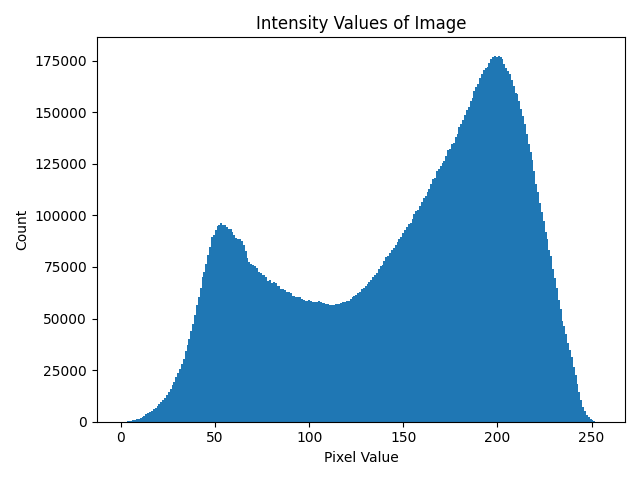
\includegraphics[height=0.19\textheight]{figures/pixel-values.png}\label{fig:intensity-histogram}}
	\hfill
	   \subfloat[Source Image\centering]{\includegraphics[height=0.19\textheight]{figures/pixel-values-image.jpg}
	  \label{fig:source-image}}
	\caption[Bimodal distribution of pixel intensity]{A example of a bimodal distribution of pixel intensity values. Note that there are two peaks in the histogram above (\ref{fig:intensity-histogram}), corresponding to what can be observed in \ref{fig:source-image}, where there are only two classes of pixels visible: crop and ground.}
	\label{fig:intensity}
\end{figure*}

%\begin{multline}
%\sigma^2_\omega (t) = \omega_0(t)\sigma^2_0 (t) + \omega_1 (t) \sigma^2_1 (t) \\
%where 
%\end{multline}
%
Otsu's method operates on the assumption that there are two classes of pixels in the object (interesting and uninteresting things). The algorithm minimizes intra-class variance. This method performs well when presented with images that have two distinct peaks
% Equation from https://infoaryan.com/blog/opencv-python-otsu-and-triangle-thresholding-full-mathematics-code-explained-important/
\begin{equation}
\sigma^2_B (t) \times p(t) \times p(\overline{t}) \\
\end{equation}
where $\sigma^2_B (t)$ is the variance between the two classes, $p(t)$ is the probability of class $t$, and $p(\overline{t})$ is the probability of the complement.

For the triangle method uses this equation:
\begin{equation}
T_{triangle} = argmax \left[ h(T) \times \left( 1 - \left| \frac{T - P}{R - P} \right| \right) \right]
\end{equation}
Where $h(T)$ is the value at $T$, $R$ is the maximum of the intensity, and $P$ is the peak value.

The details of the implentation of these two approaches are beyond the scope of this document, and while there are certainly others, these are, perhaps the most frequently encountered approaches. Both of these approaches, however, are based on some assumptions about the intensity histogram, and may not work well in all situations, particularly if these assumptions are not valid. Otsu's algorithm, for example, tends to yield satisfactory results when operating on images posessing a bimodal distribution, but may not yield good results on images with a single peak or multiple peaks.


\begin{figure}[H]
	\centering
	  \subfloat[NDI Index\centering]{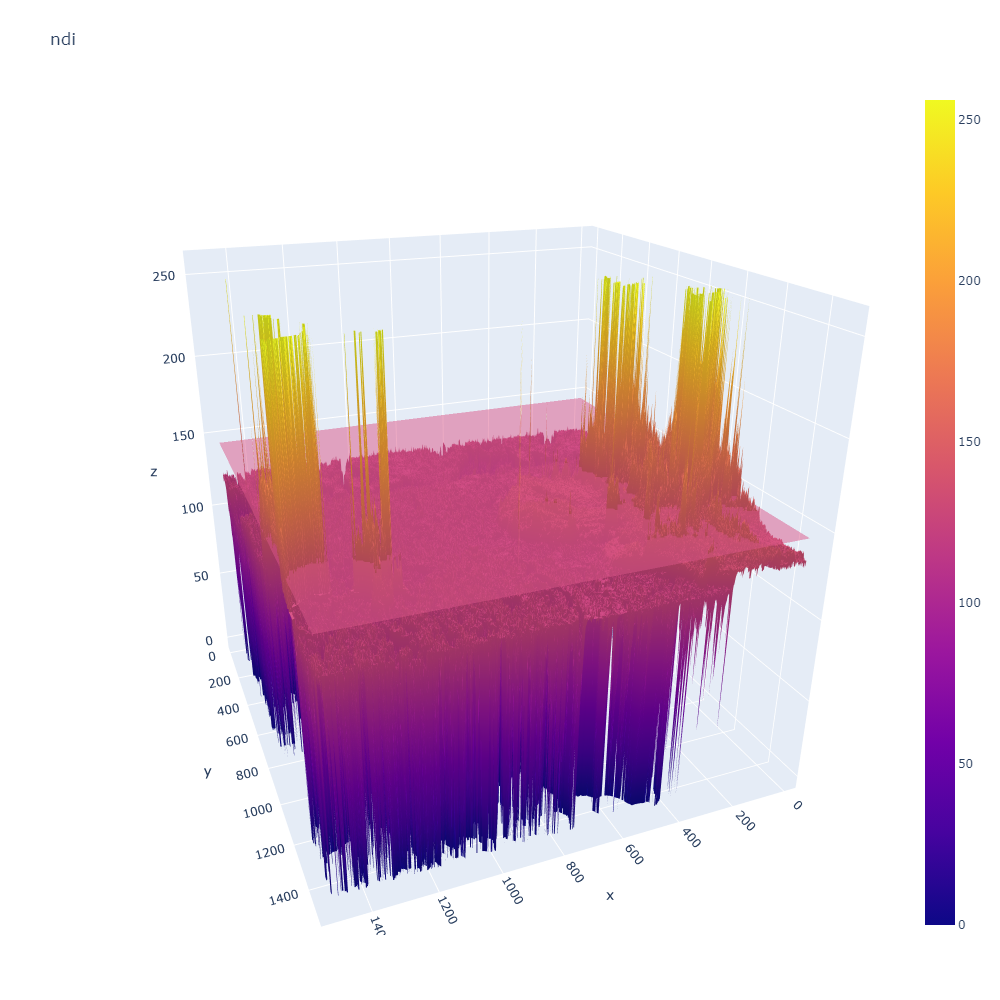
\includegraphics[height=0.19\textheight]{figures/ndi-1-of-2.png}\label{fig:ndi-1}}
	\hfill
	   \subfloat[Triangle Algorithm\centering]{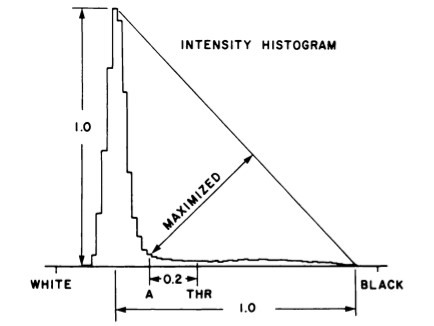
\includegraphics[height=0.19\textheight]{figures/triangle-algorithm}\label{fig:ndi-2}}
	\caption[NDI segmentation and threshold selection]{An example of NDI segmentation and threshold selection. A threshold for the production of a mask can be done manually, perhaps by selecting all values below 140 (noted by the translucent pink plane in \ref{fig:ndi-1}) to form the mask that will be applied to the image, illustrated by the semi-opaque plane. While that manual selection may be sufficient to perform the segmentation of an image set acquired under the same ambient conditions, it may lead to the exclusion of portions of the plant in images taken under different conditions. Using the Triangle algorithm \cite{Brink1996-xy,Zack1977-yl} or Otsu's algorithm allows this selection to be made automatically. The point at which the line between the lowest and highest points in the histogram is selected as the threshold, selecting a threshold applicable to each image in a set rather than a global value used for all images in a set.}
	\label{fig:ndi-segmentation}
\end{figure}

\begin{figure}[H]
\centering
\begin{tabular}{ccc}
\subfloat[NDI]{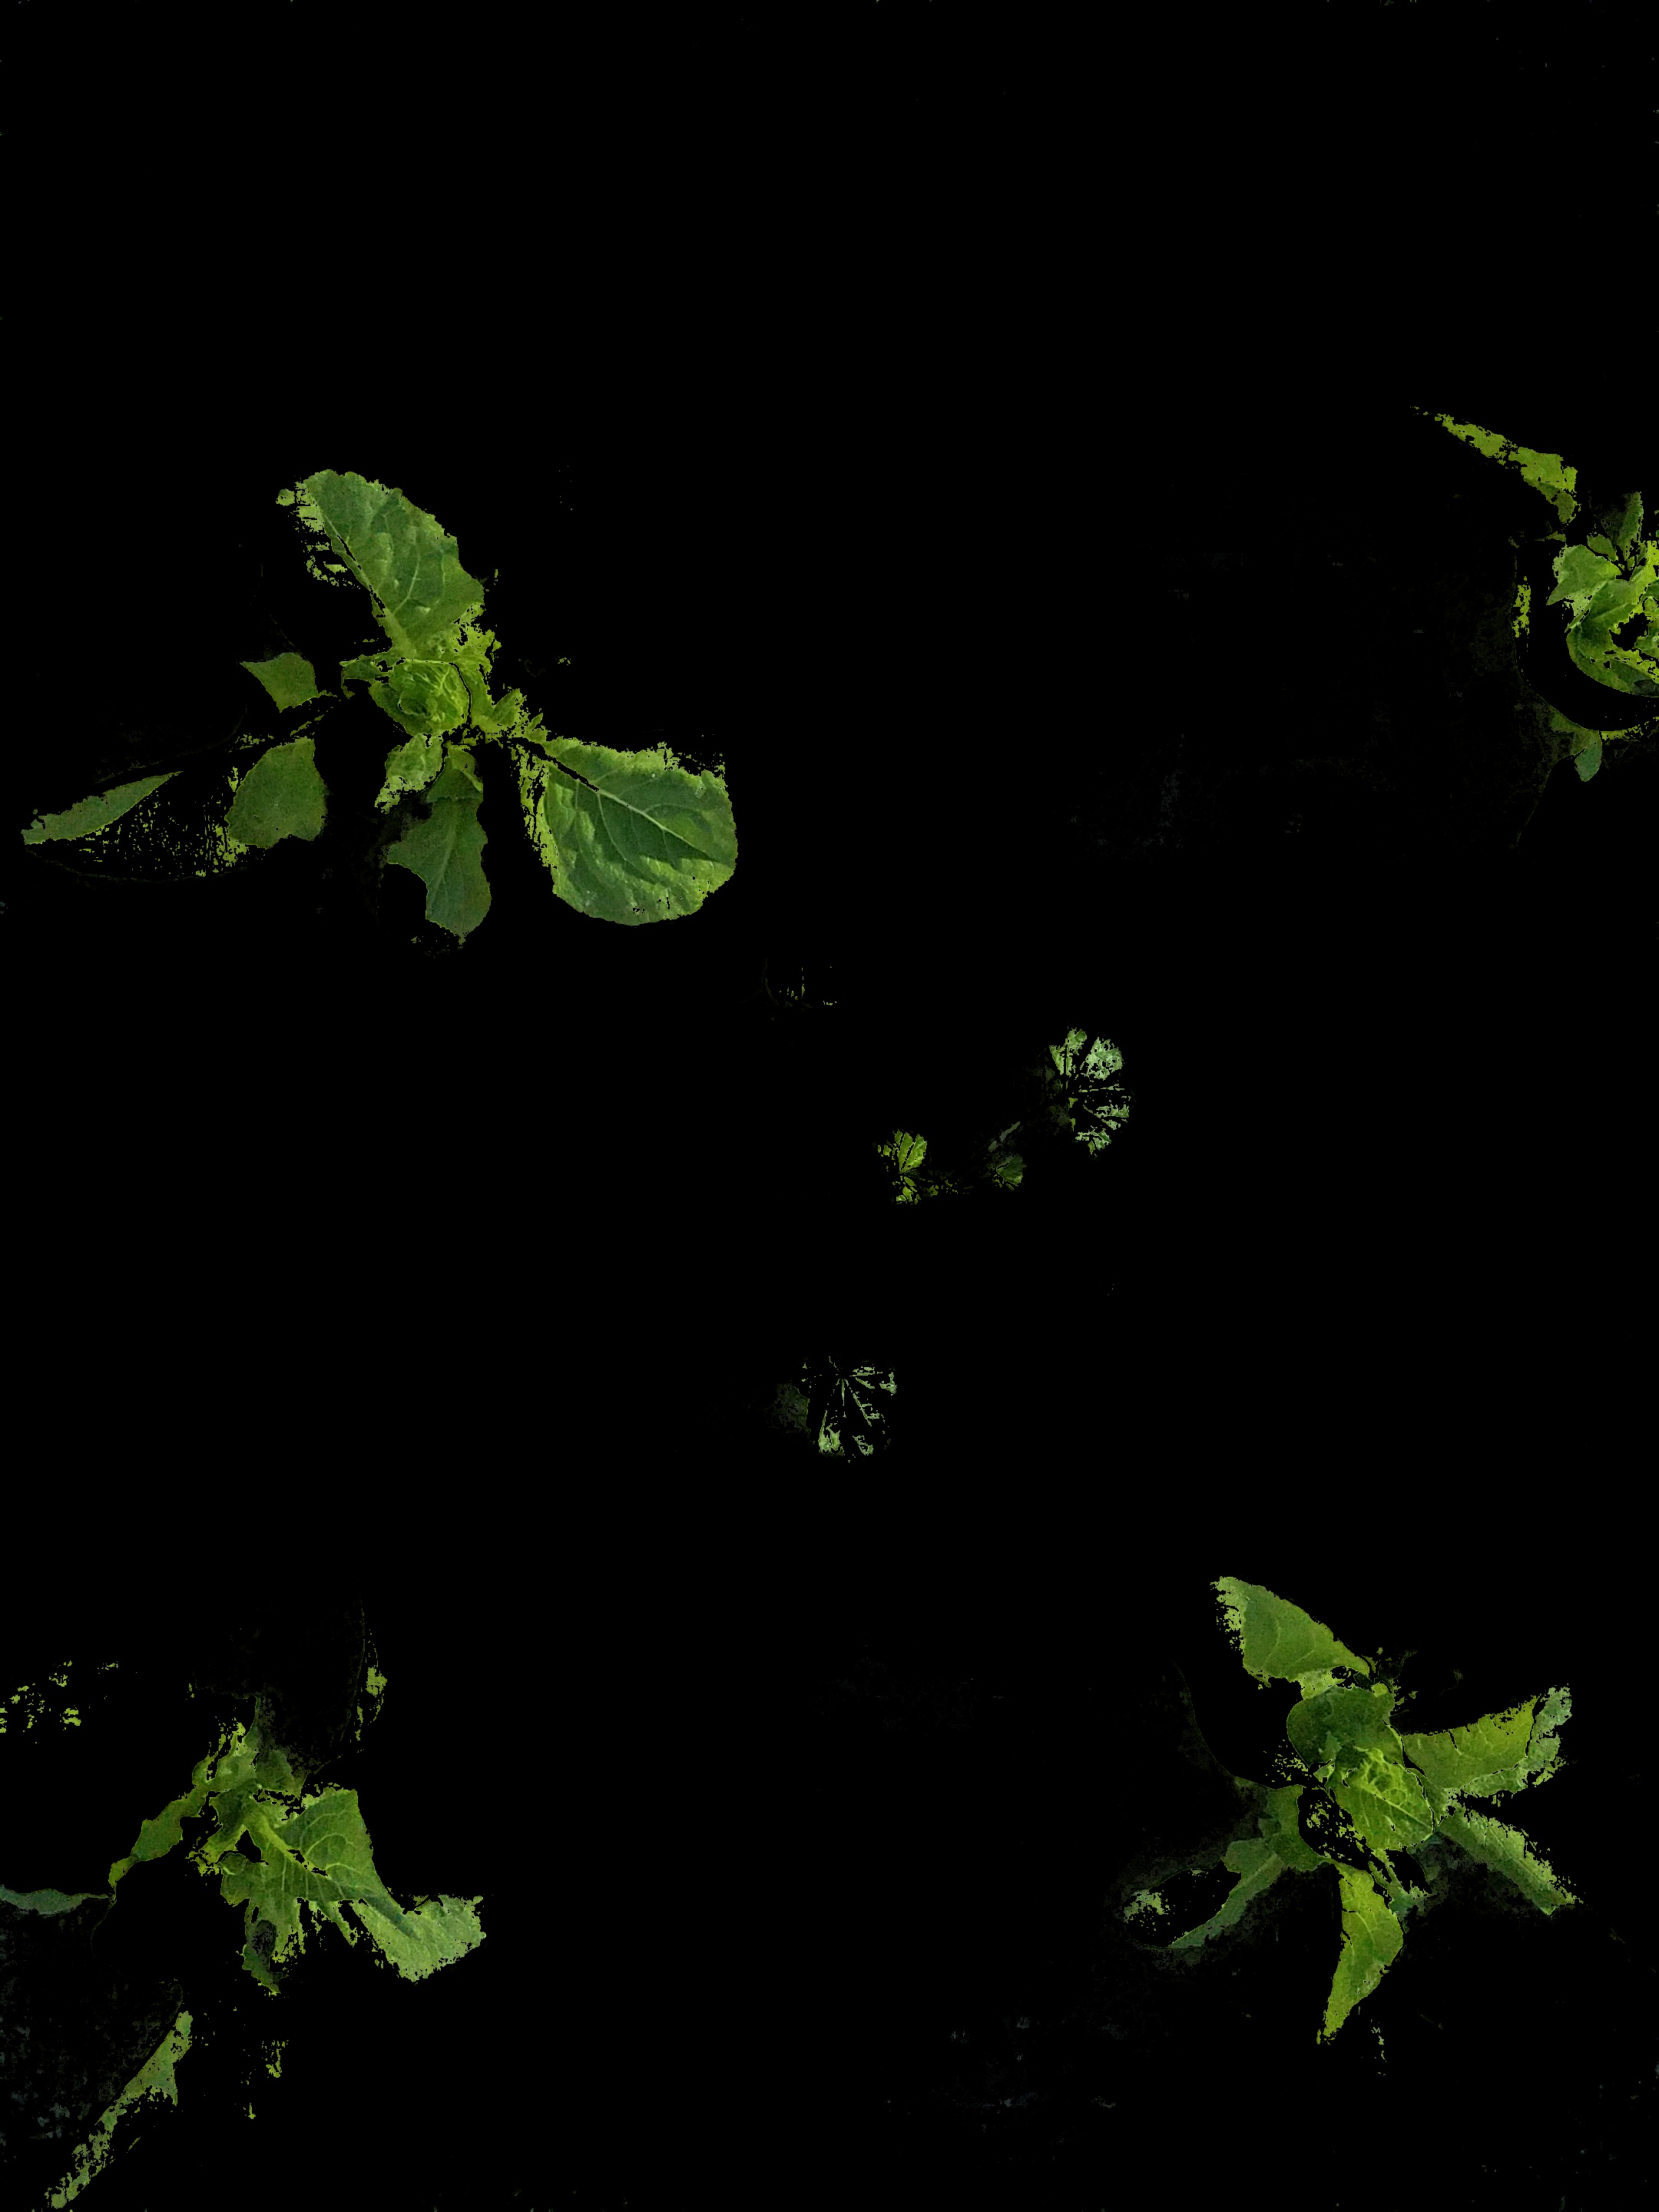
\includegraphics[width = 1.25in]{figures/20201117_112624-NDI.jpg} \label{fig:ndi}} &
\subfloat[EXG]{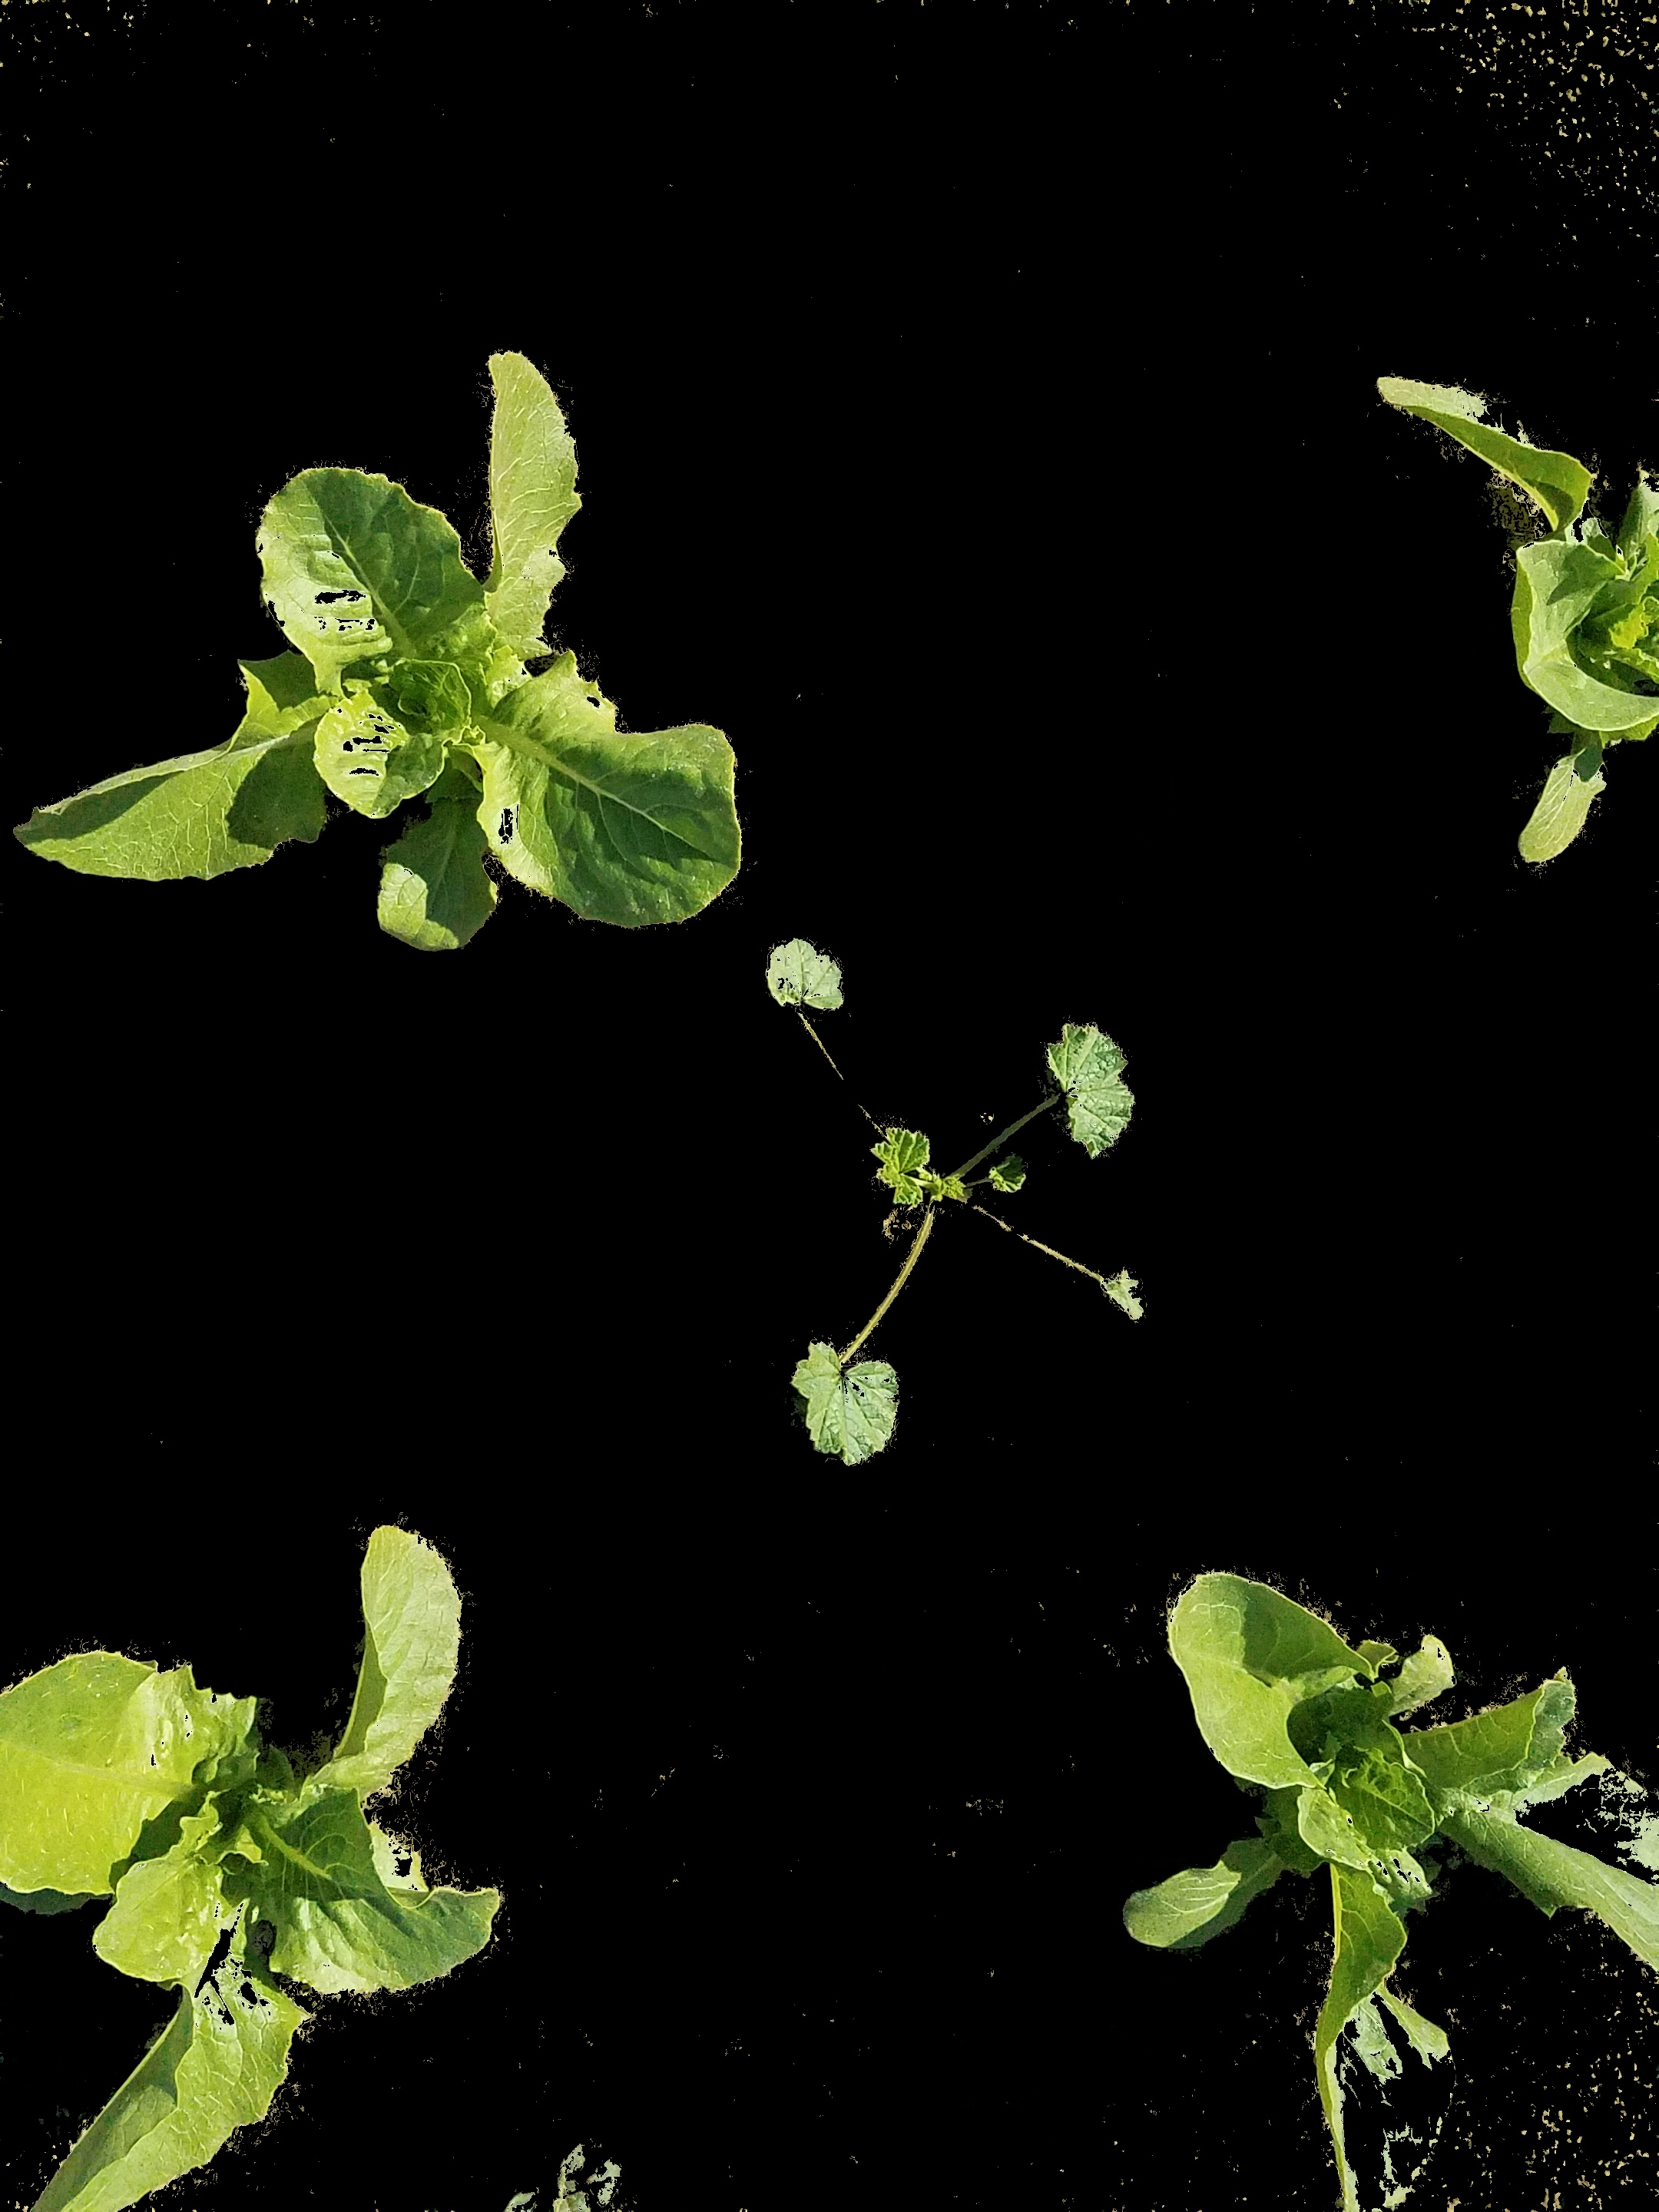
\includegraphics[width = 1.25in]{figures/20201117_112624-ExG.jpg} \label{fig:exg}} &
\subfloat[EXR]{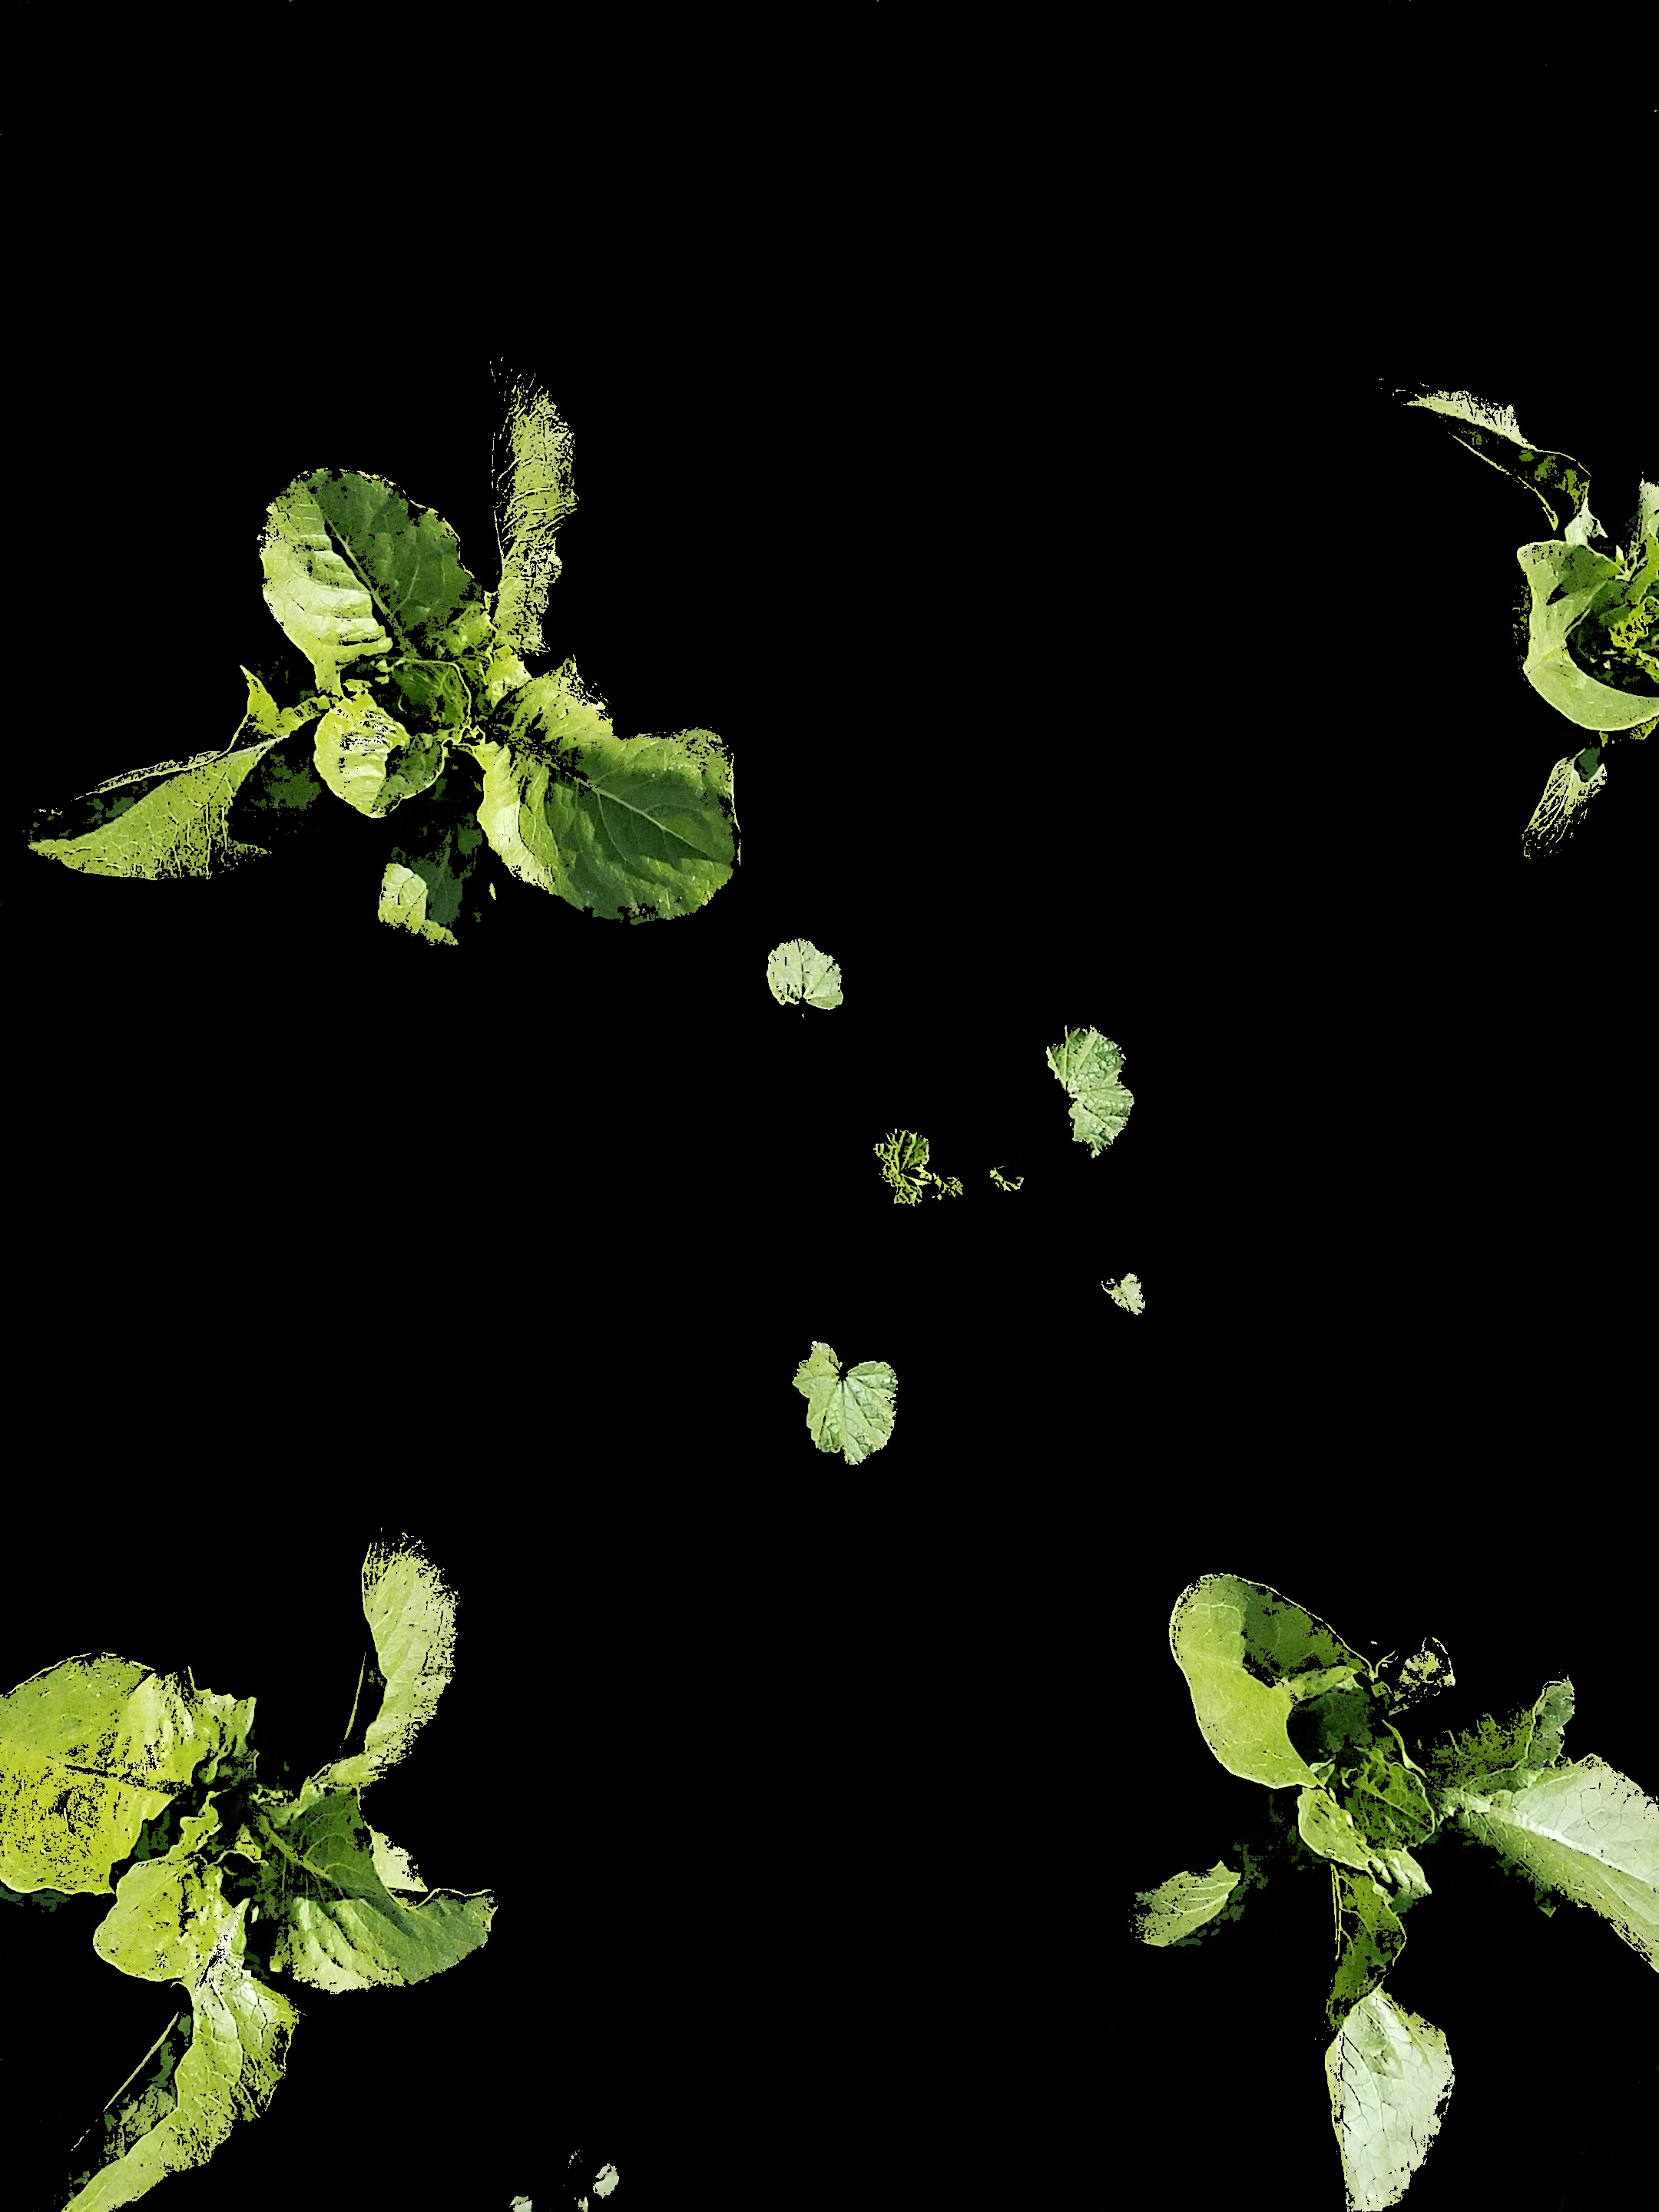
\includegraphics[width = 1.25in]{figures/20201117_112624-ExR.jpg} \label{fig:exr}} \\
\subfloat[CIVE]{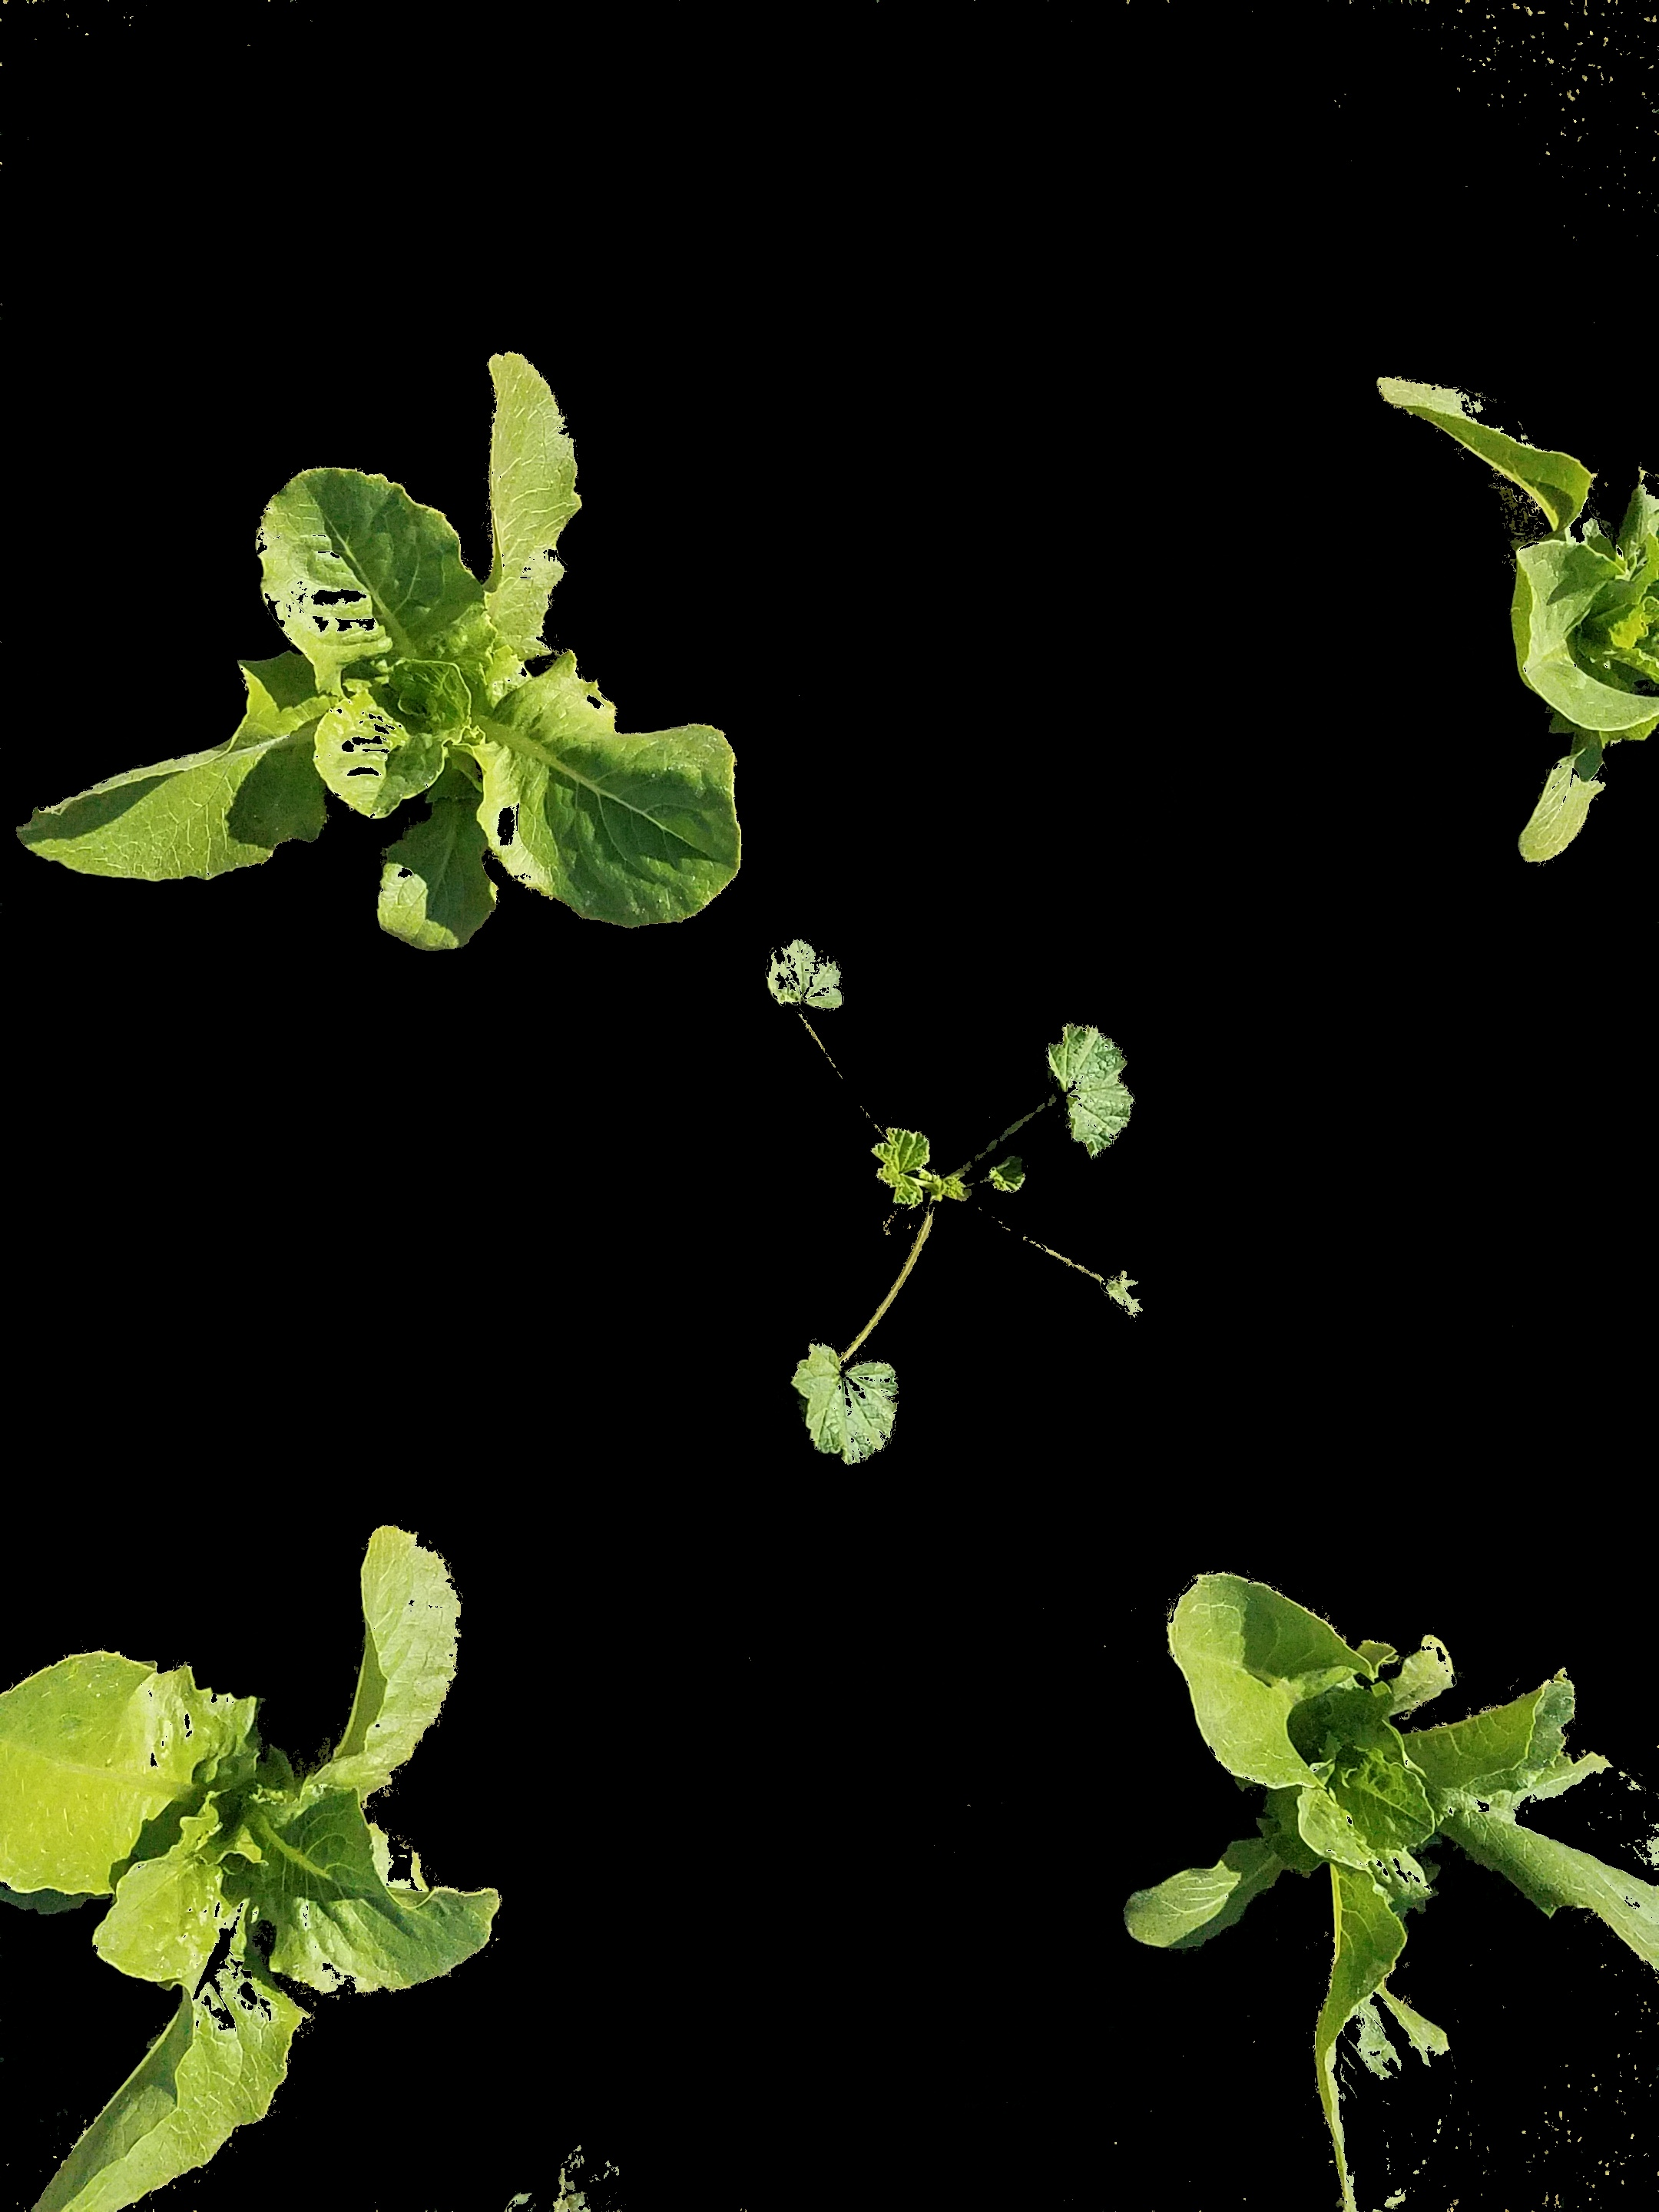
\includegraphics[width = 1.25in]{figures/20201117_112624-CIVE.jpg} \label{fig:cive}} &
\subfloat[EXG-EXR]{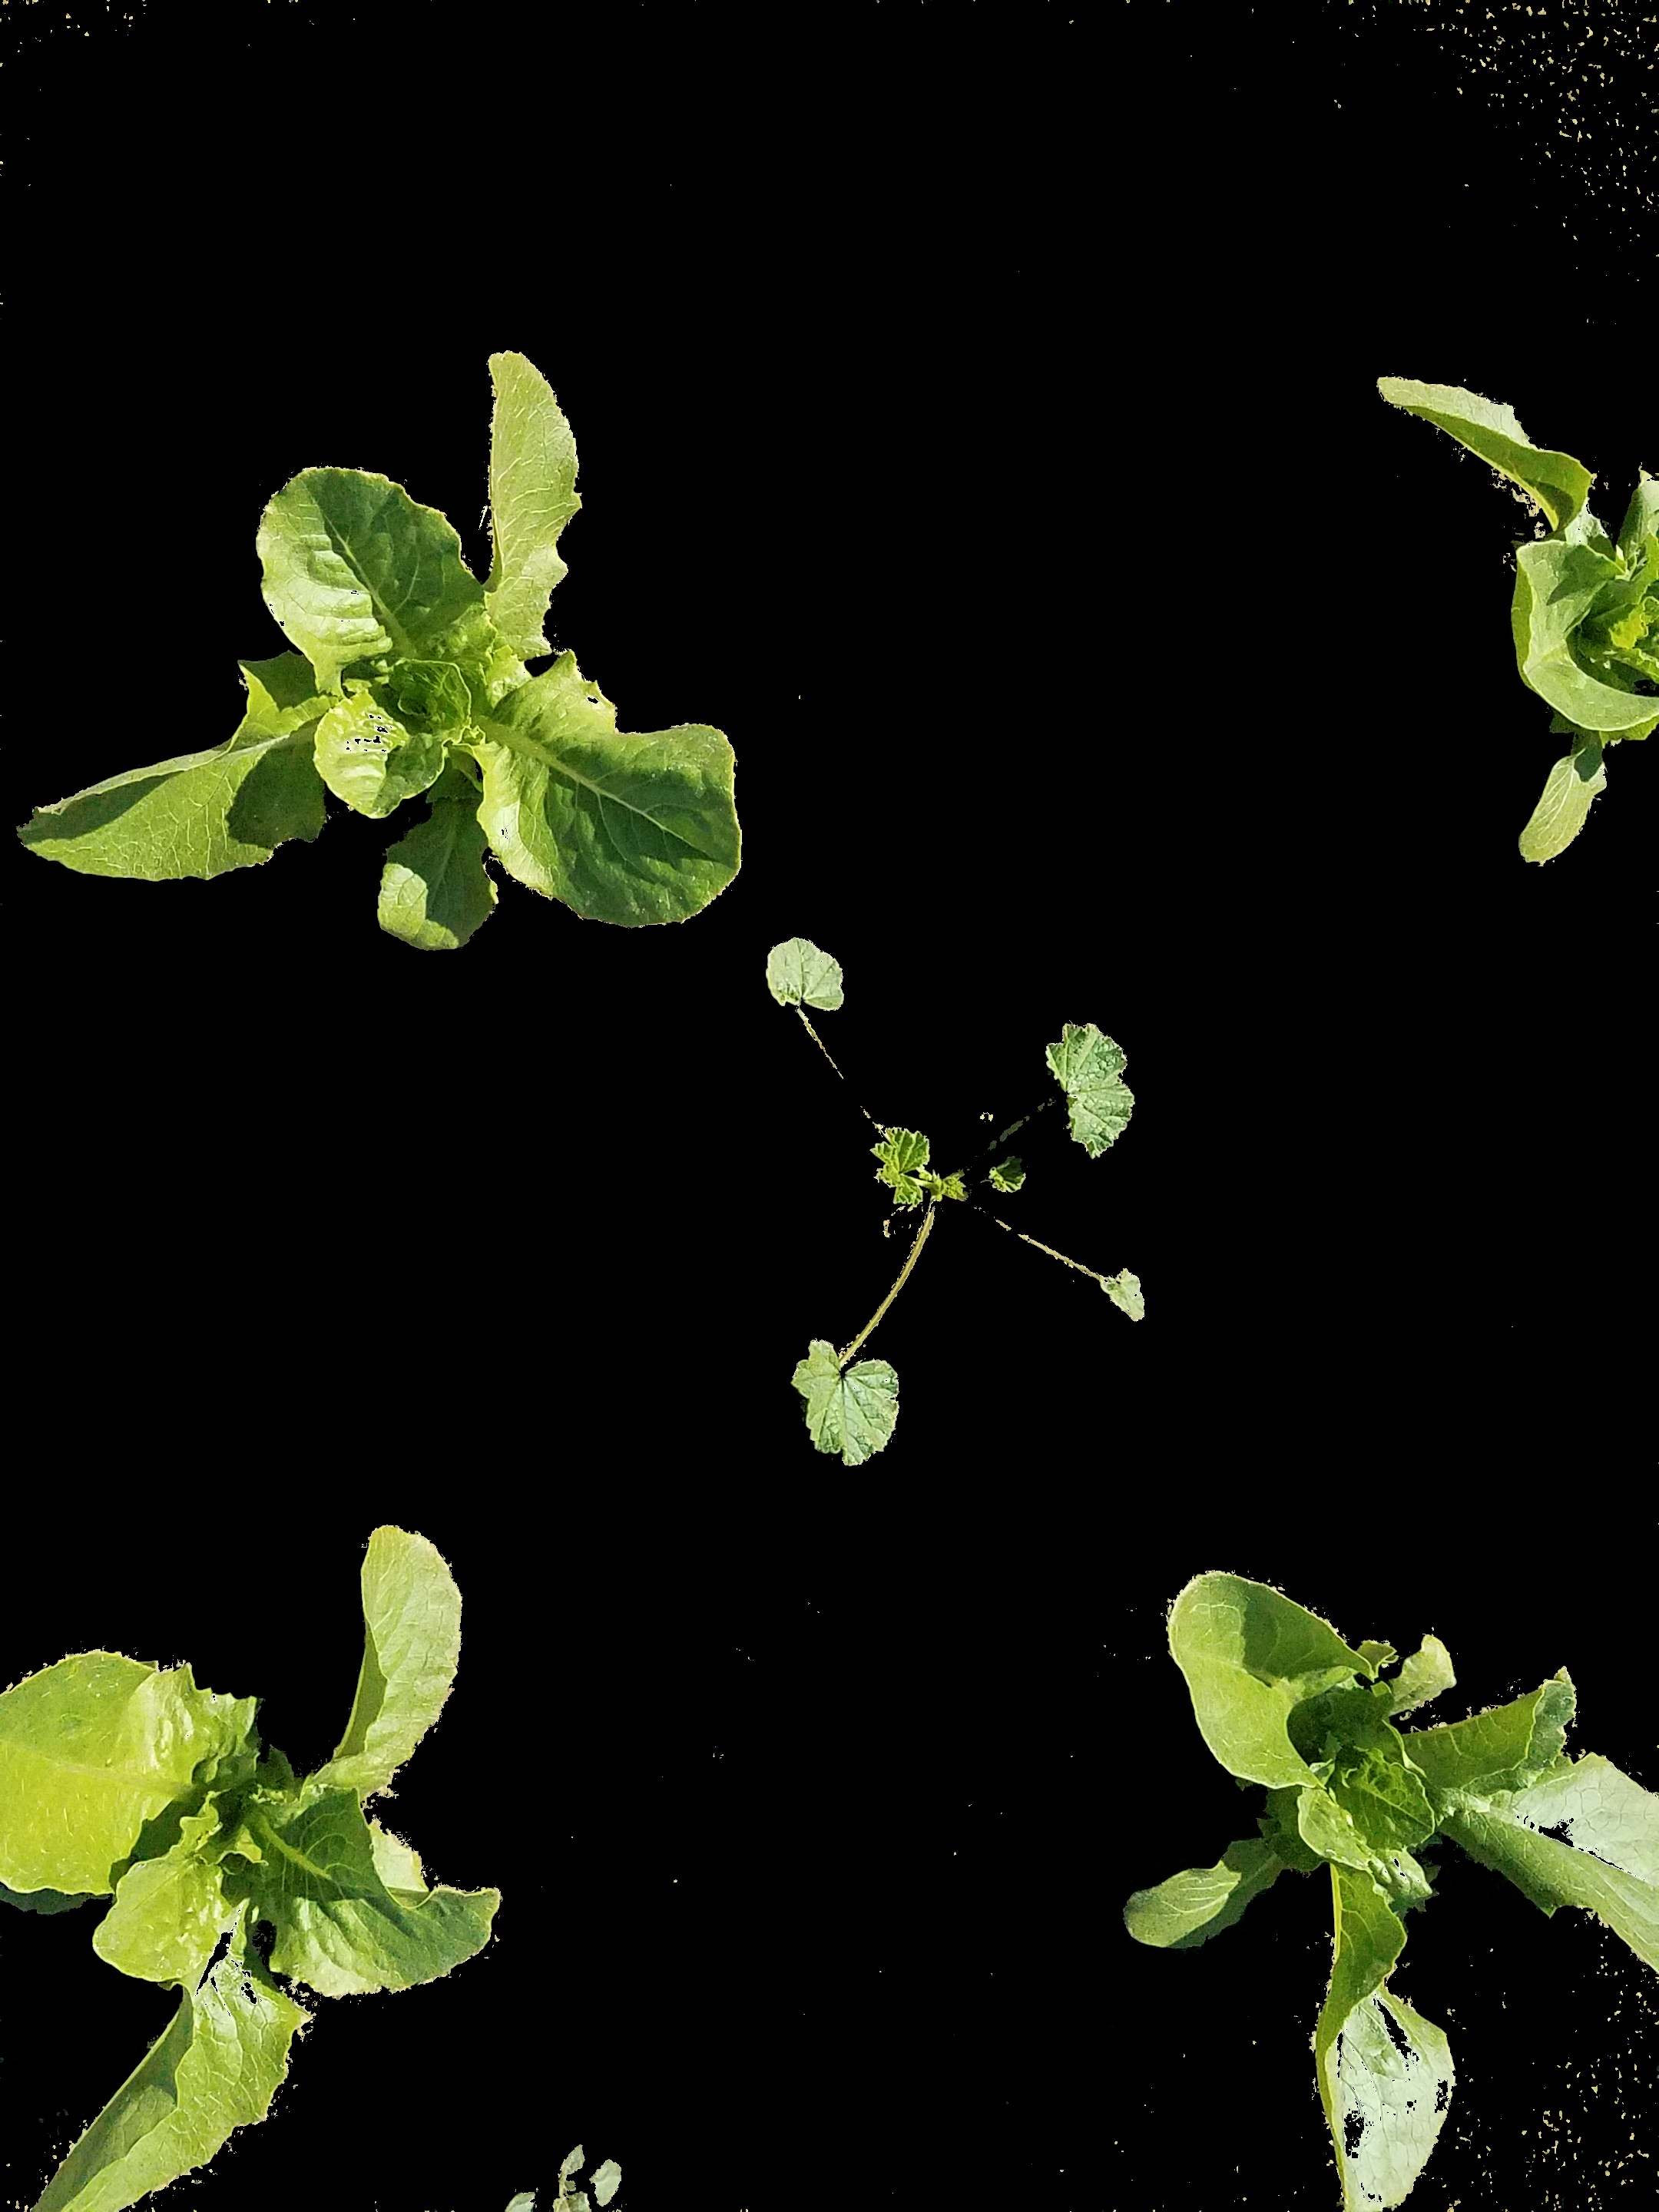
\includegraphics[width = 1.25in]{figures/20201117_112624-ExGR.jpg} \label{fig:exgexr}} &
\subfloat[NGRDI]{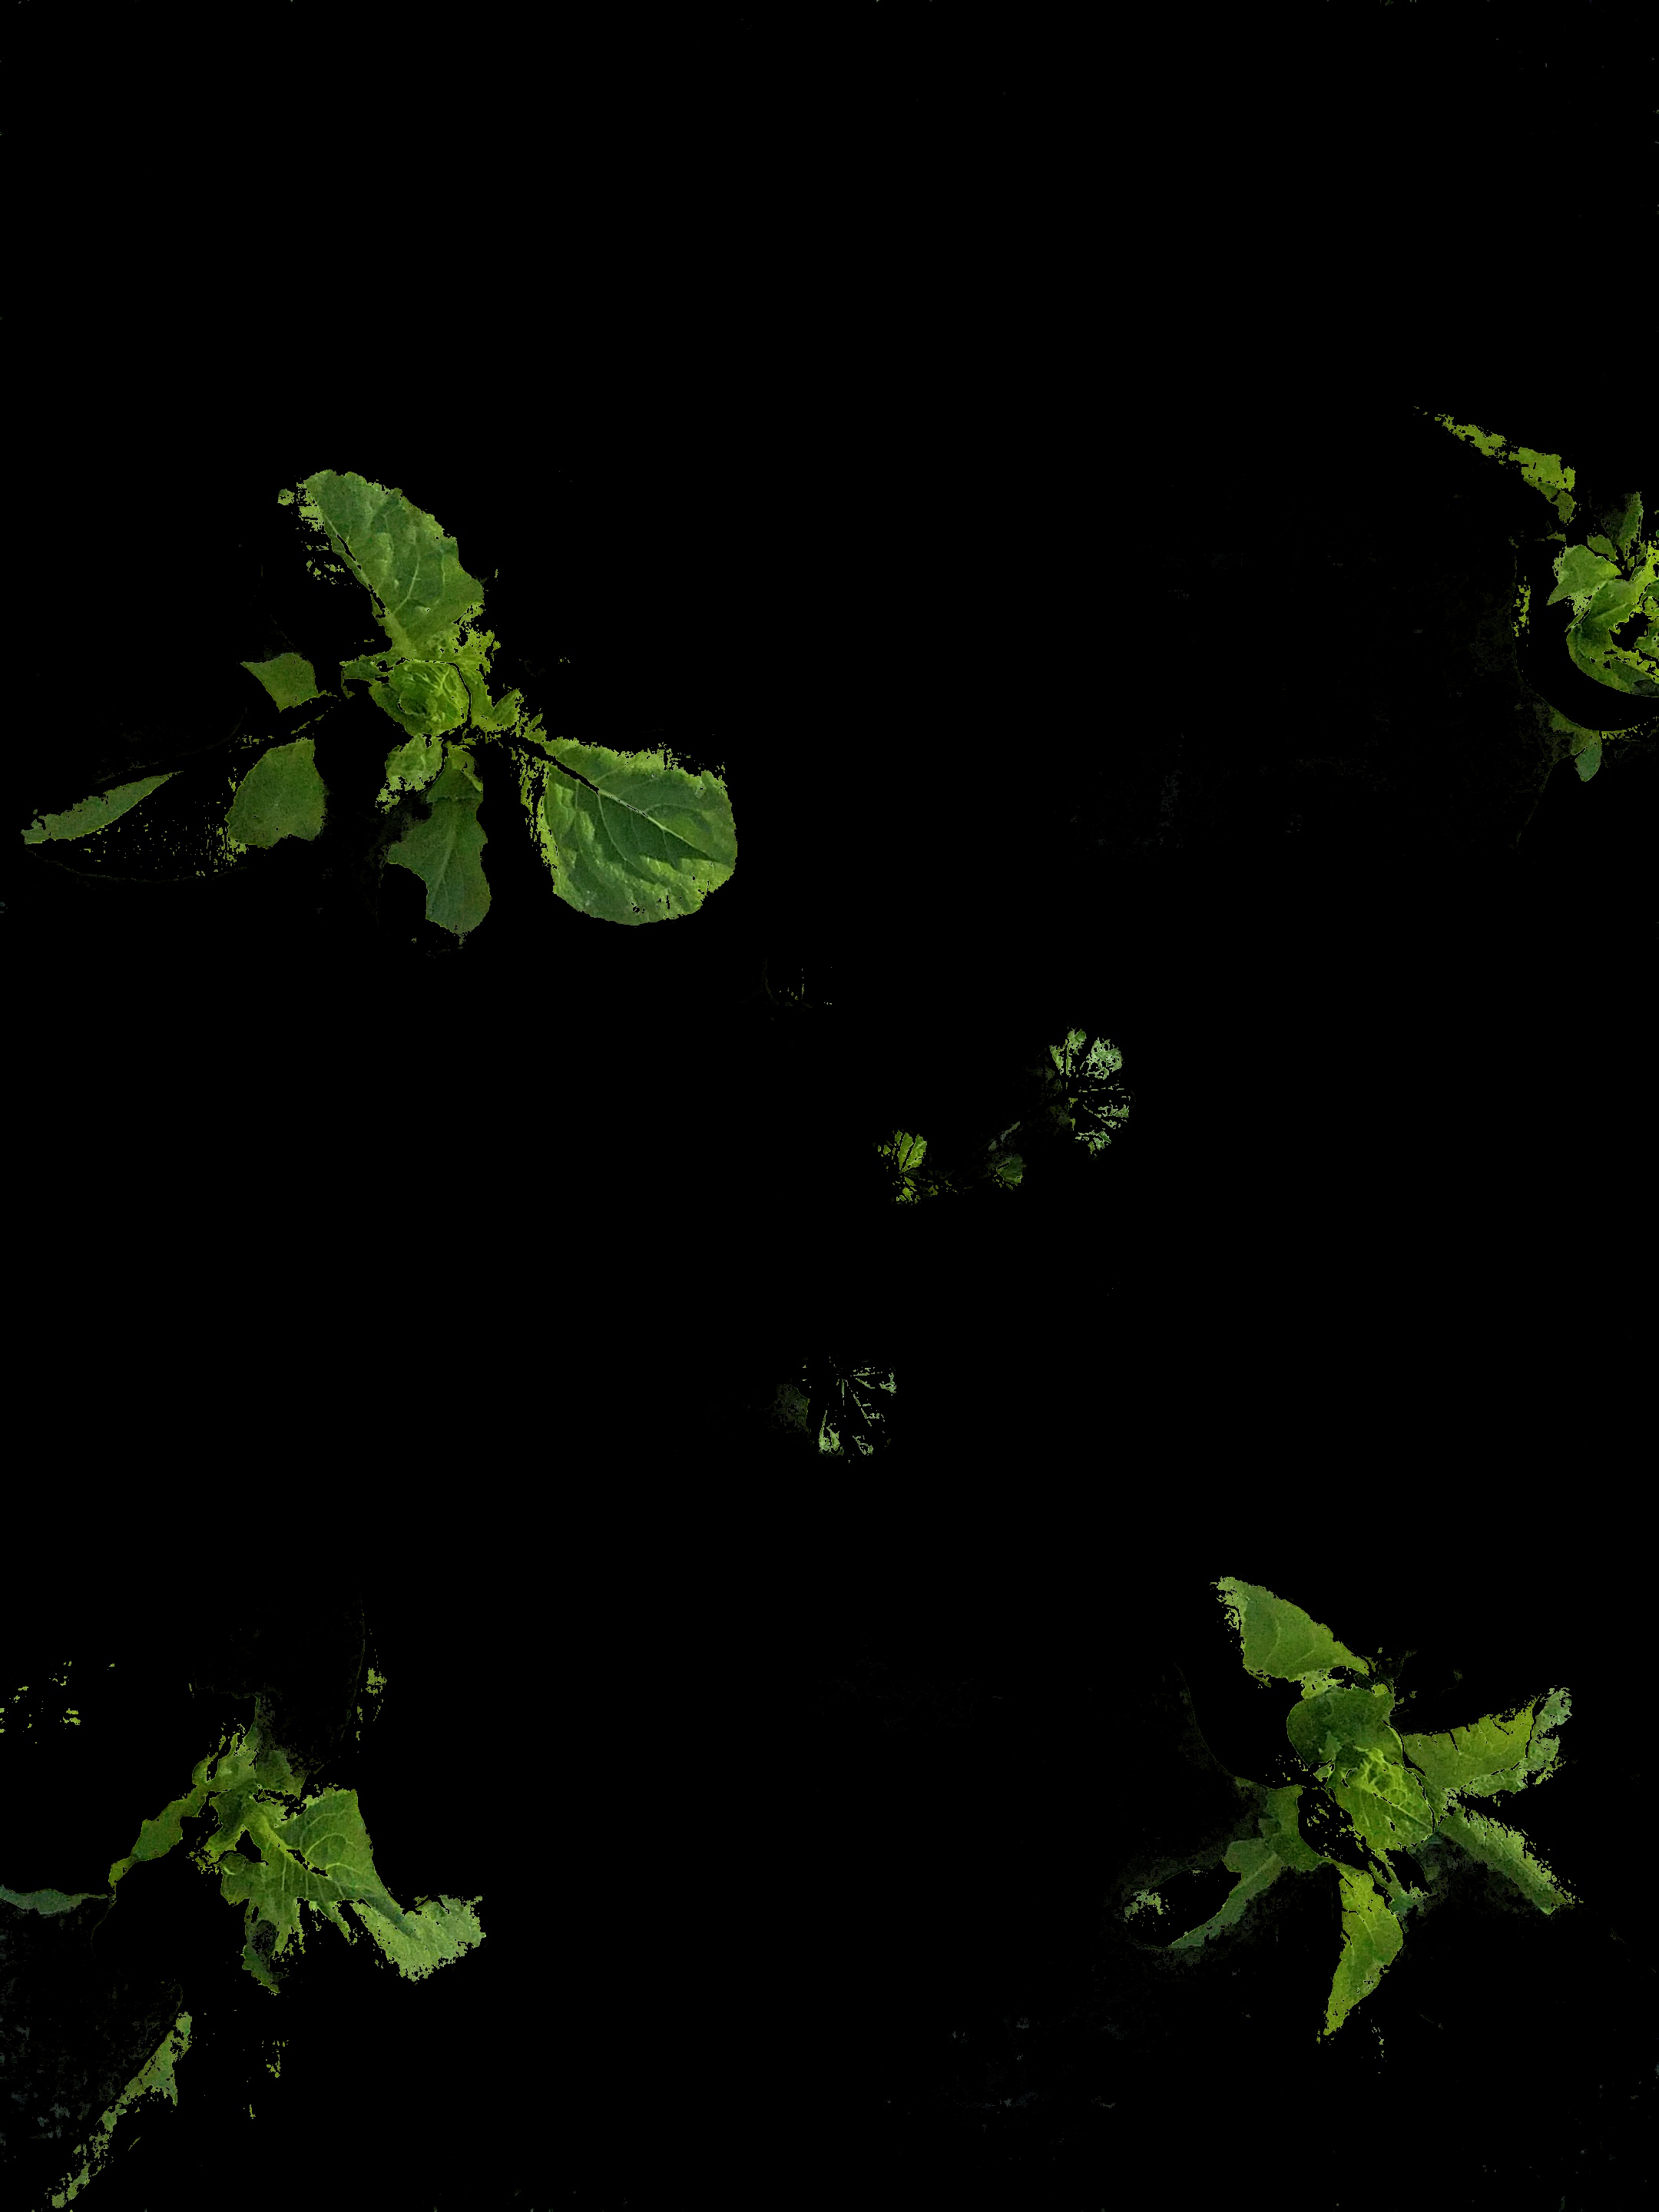
\includegraphics[width = 1.25in]{figures/20201117_112624-NGRDI.jpg} \label{fig:nrgdi}} \\
\subfloat[Com1]{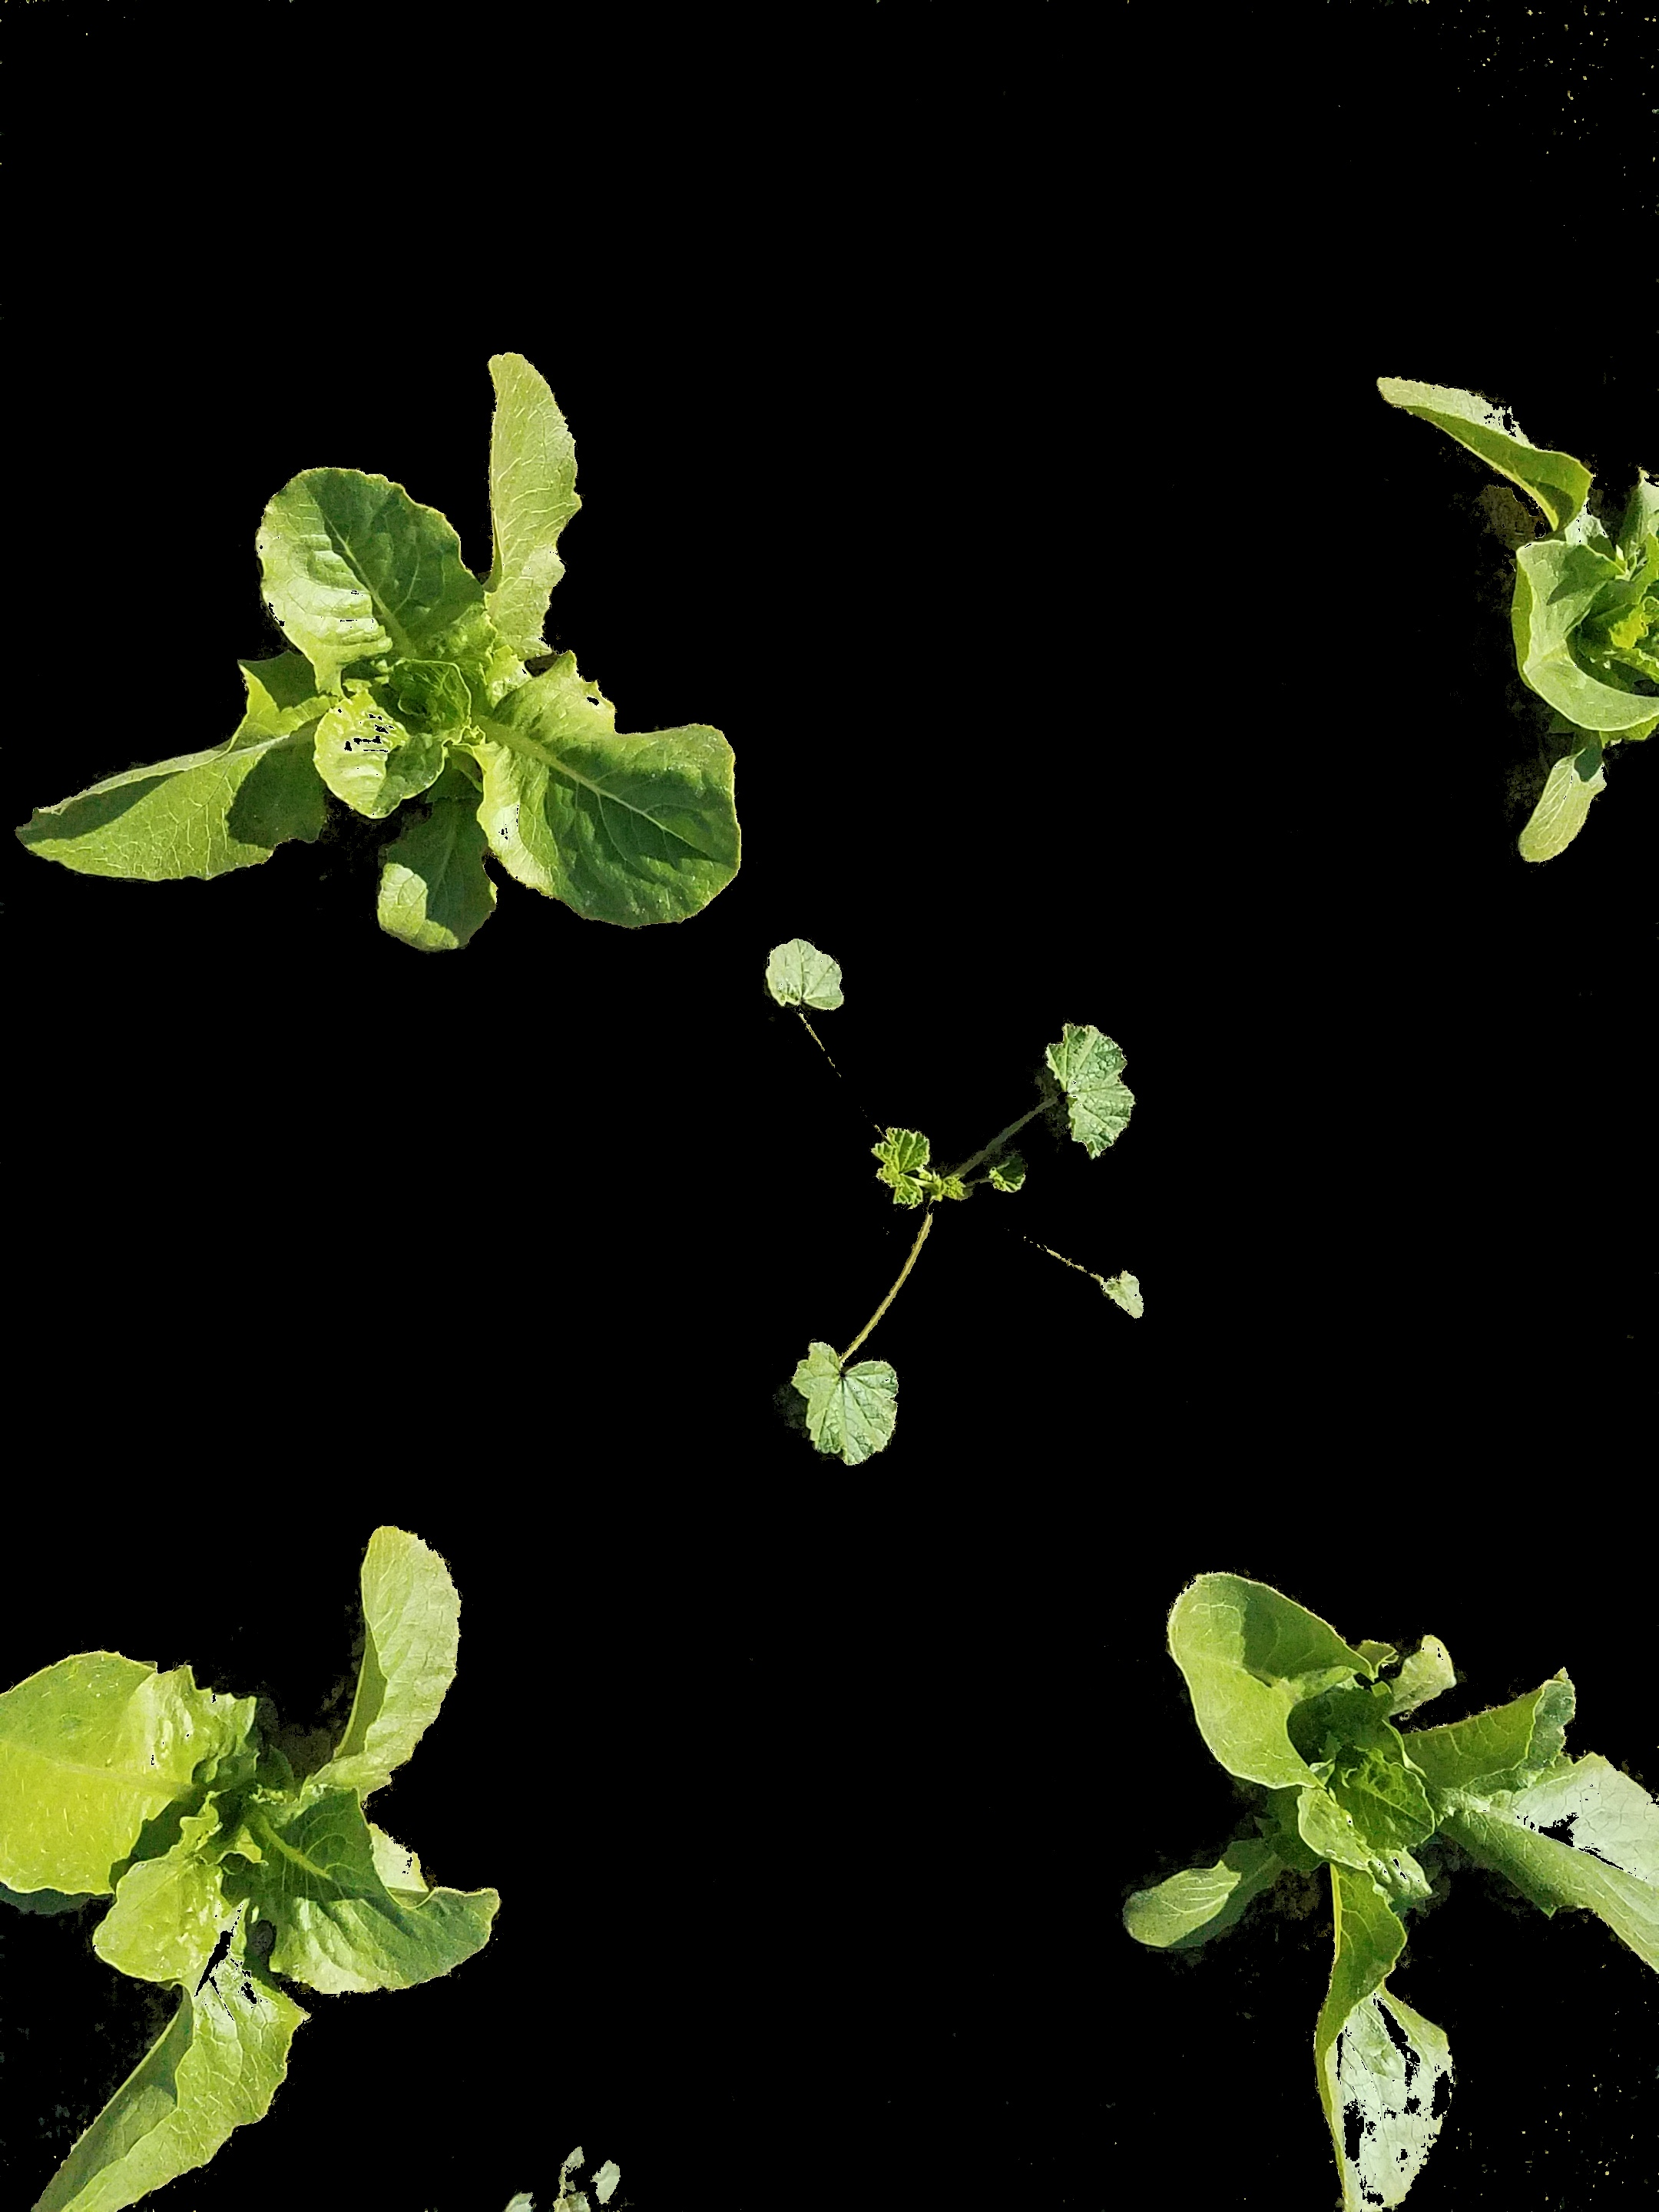
\includegraphics[width = 1.25in]{figures/20201117_112624-COM1.jpg} \label{fig:com1}} &
\subfloat[Com2]{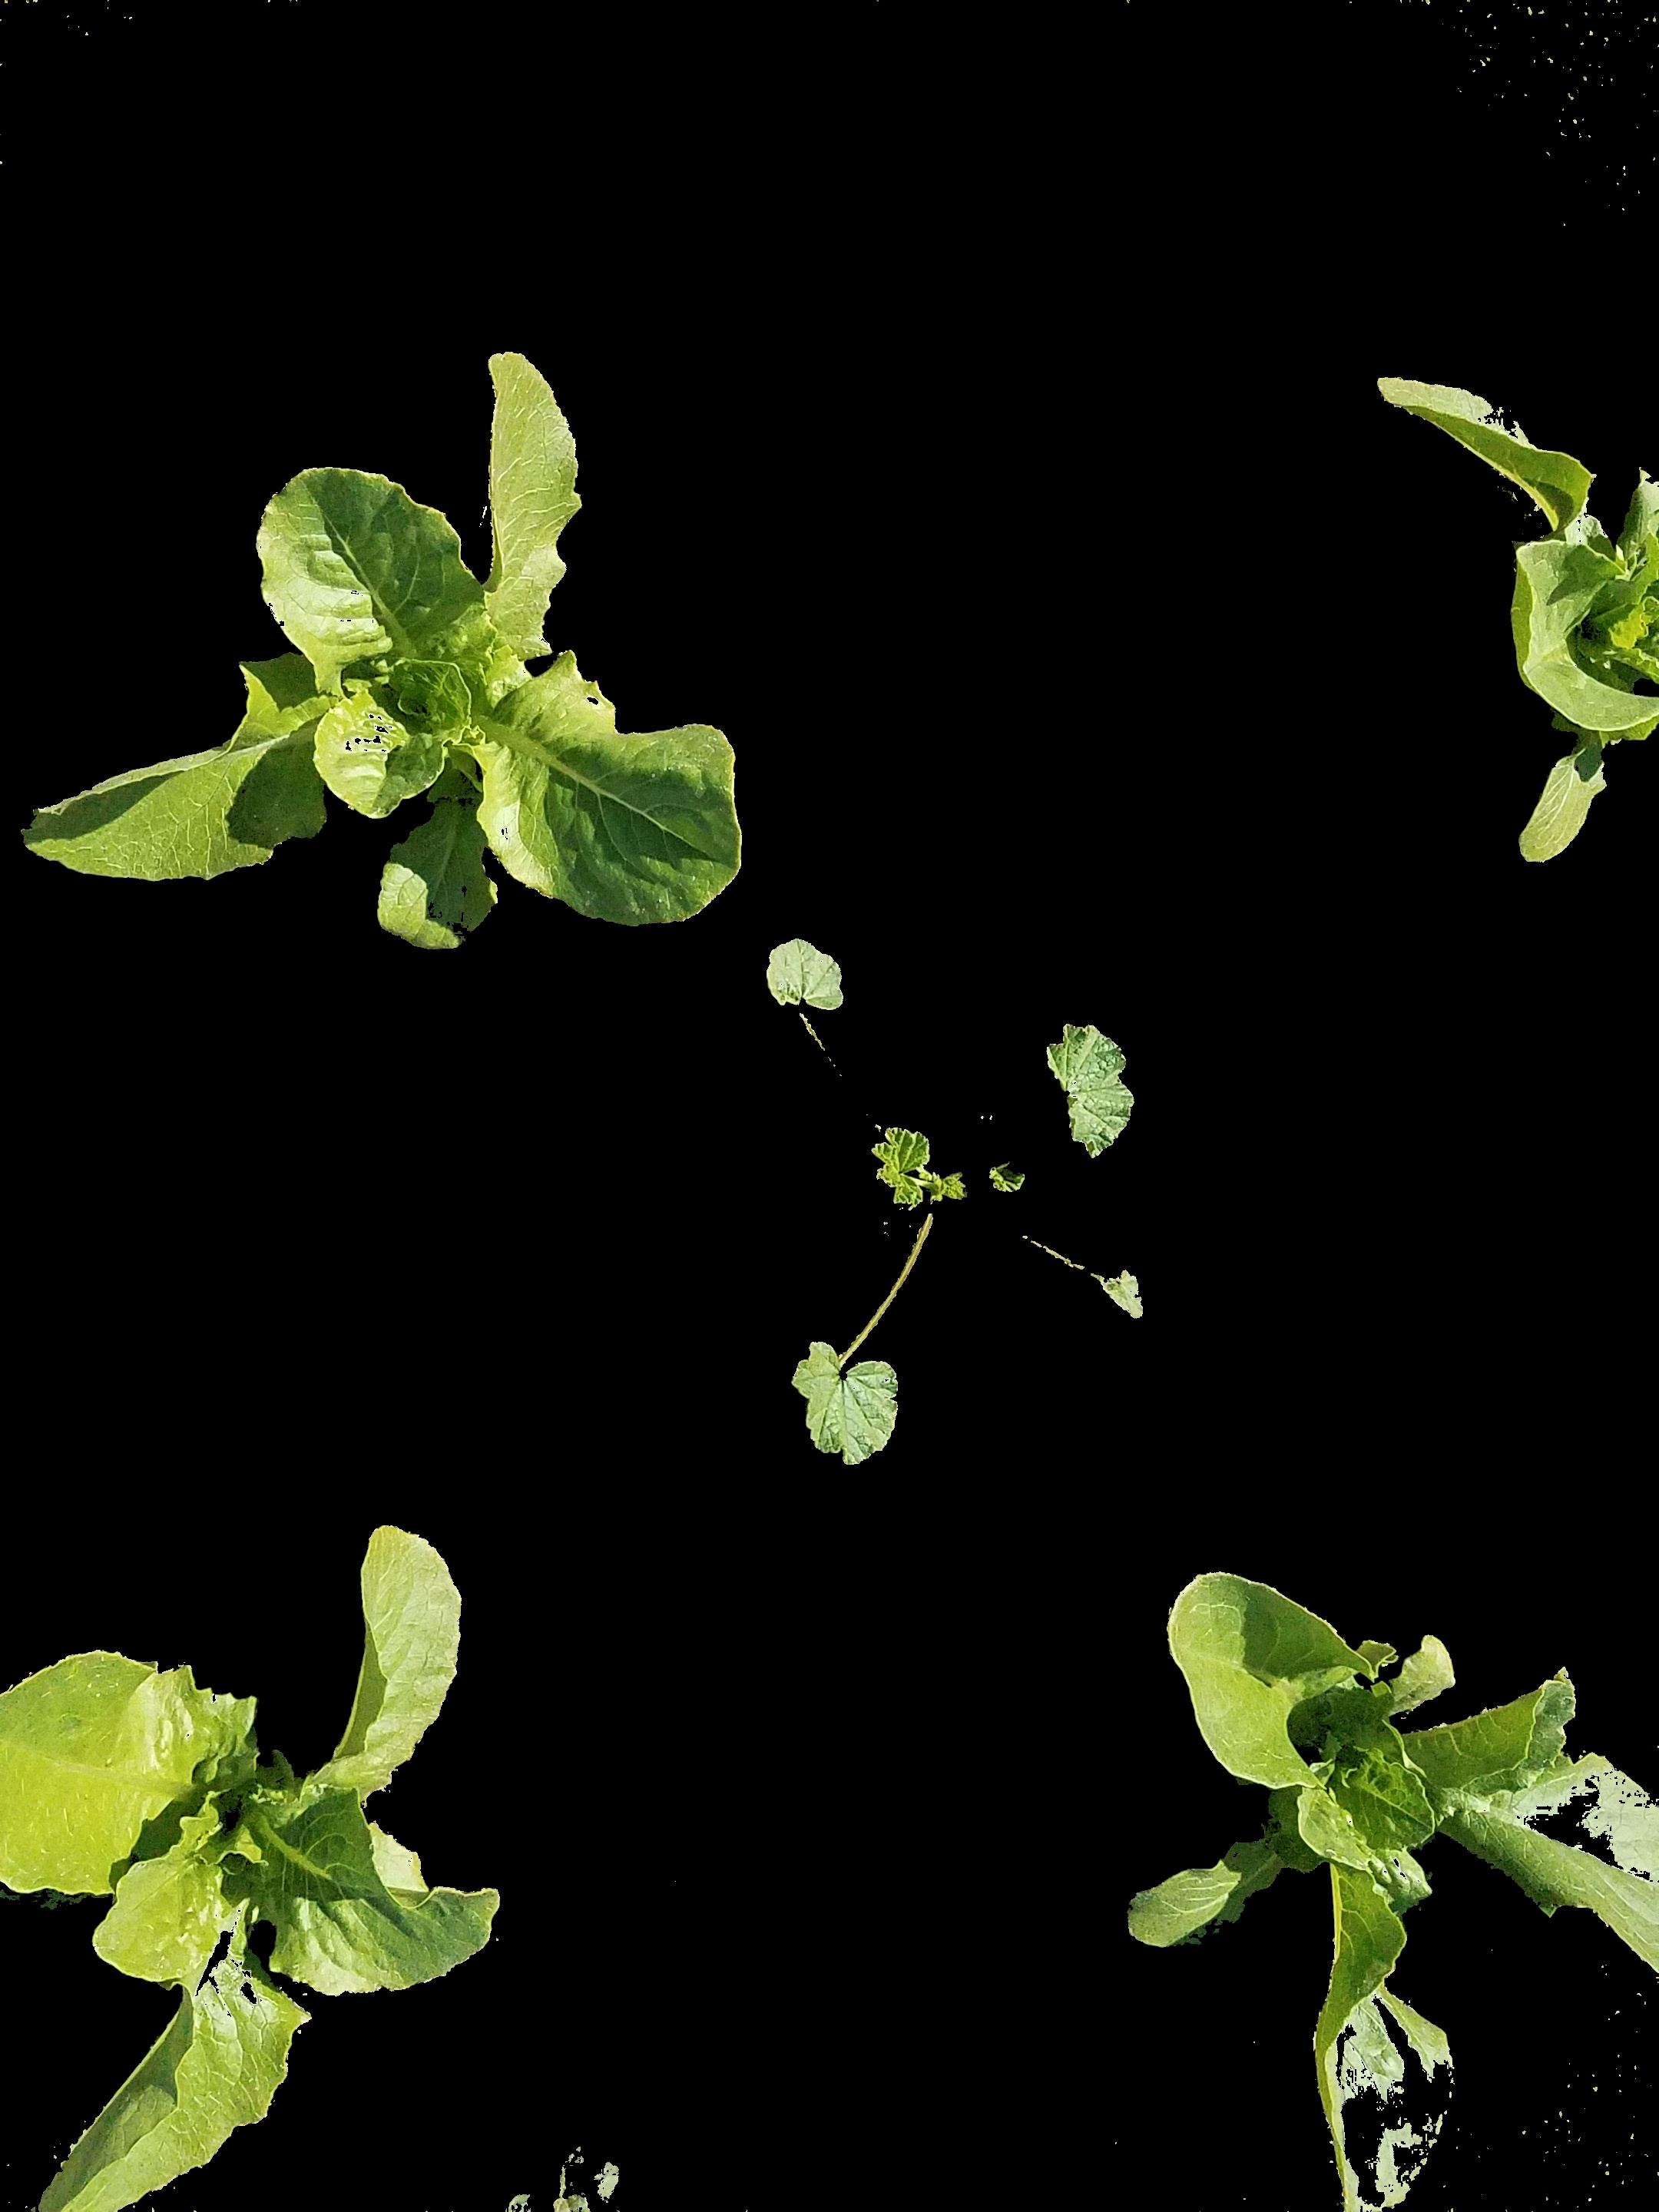
\includegraphics[width = 1.25in]{figures/20201117_112624-COM2.jpg} \label{fig:com2}}&
\subfloat[MEXG]{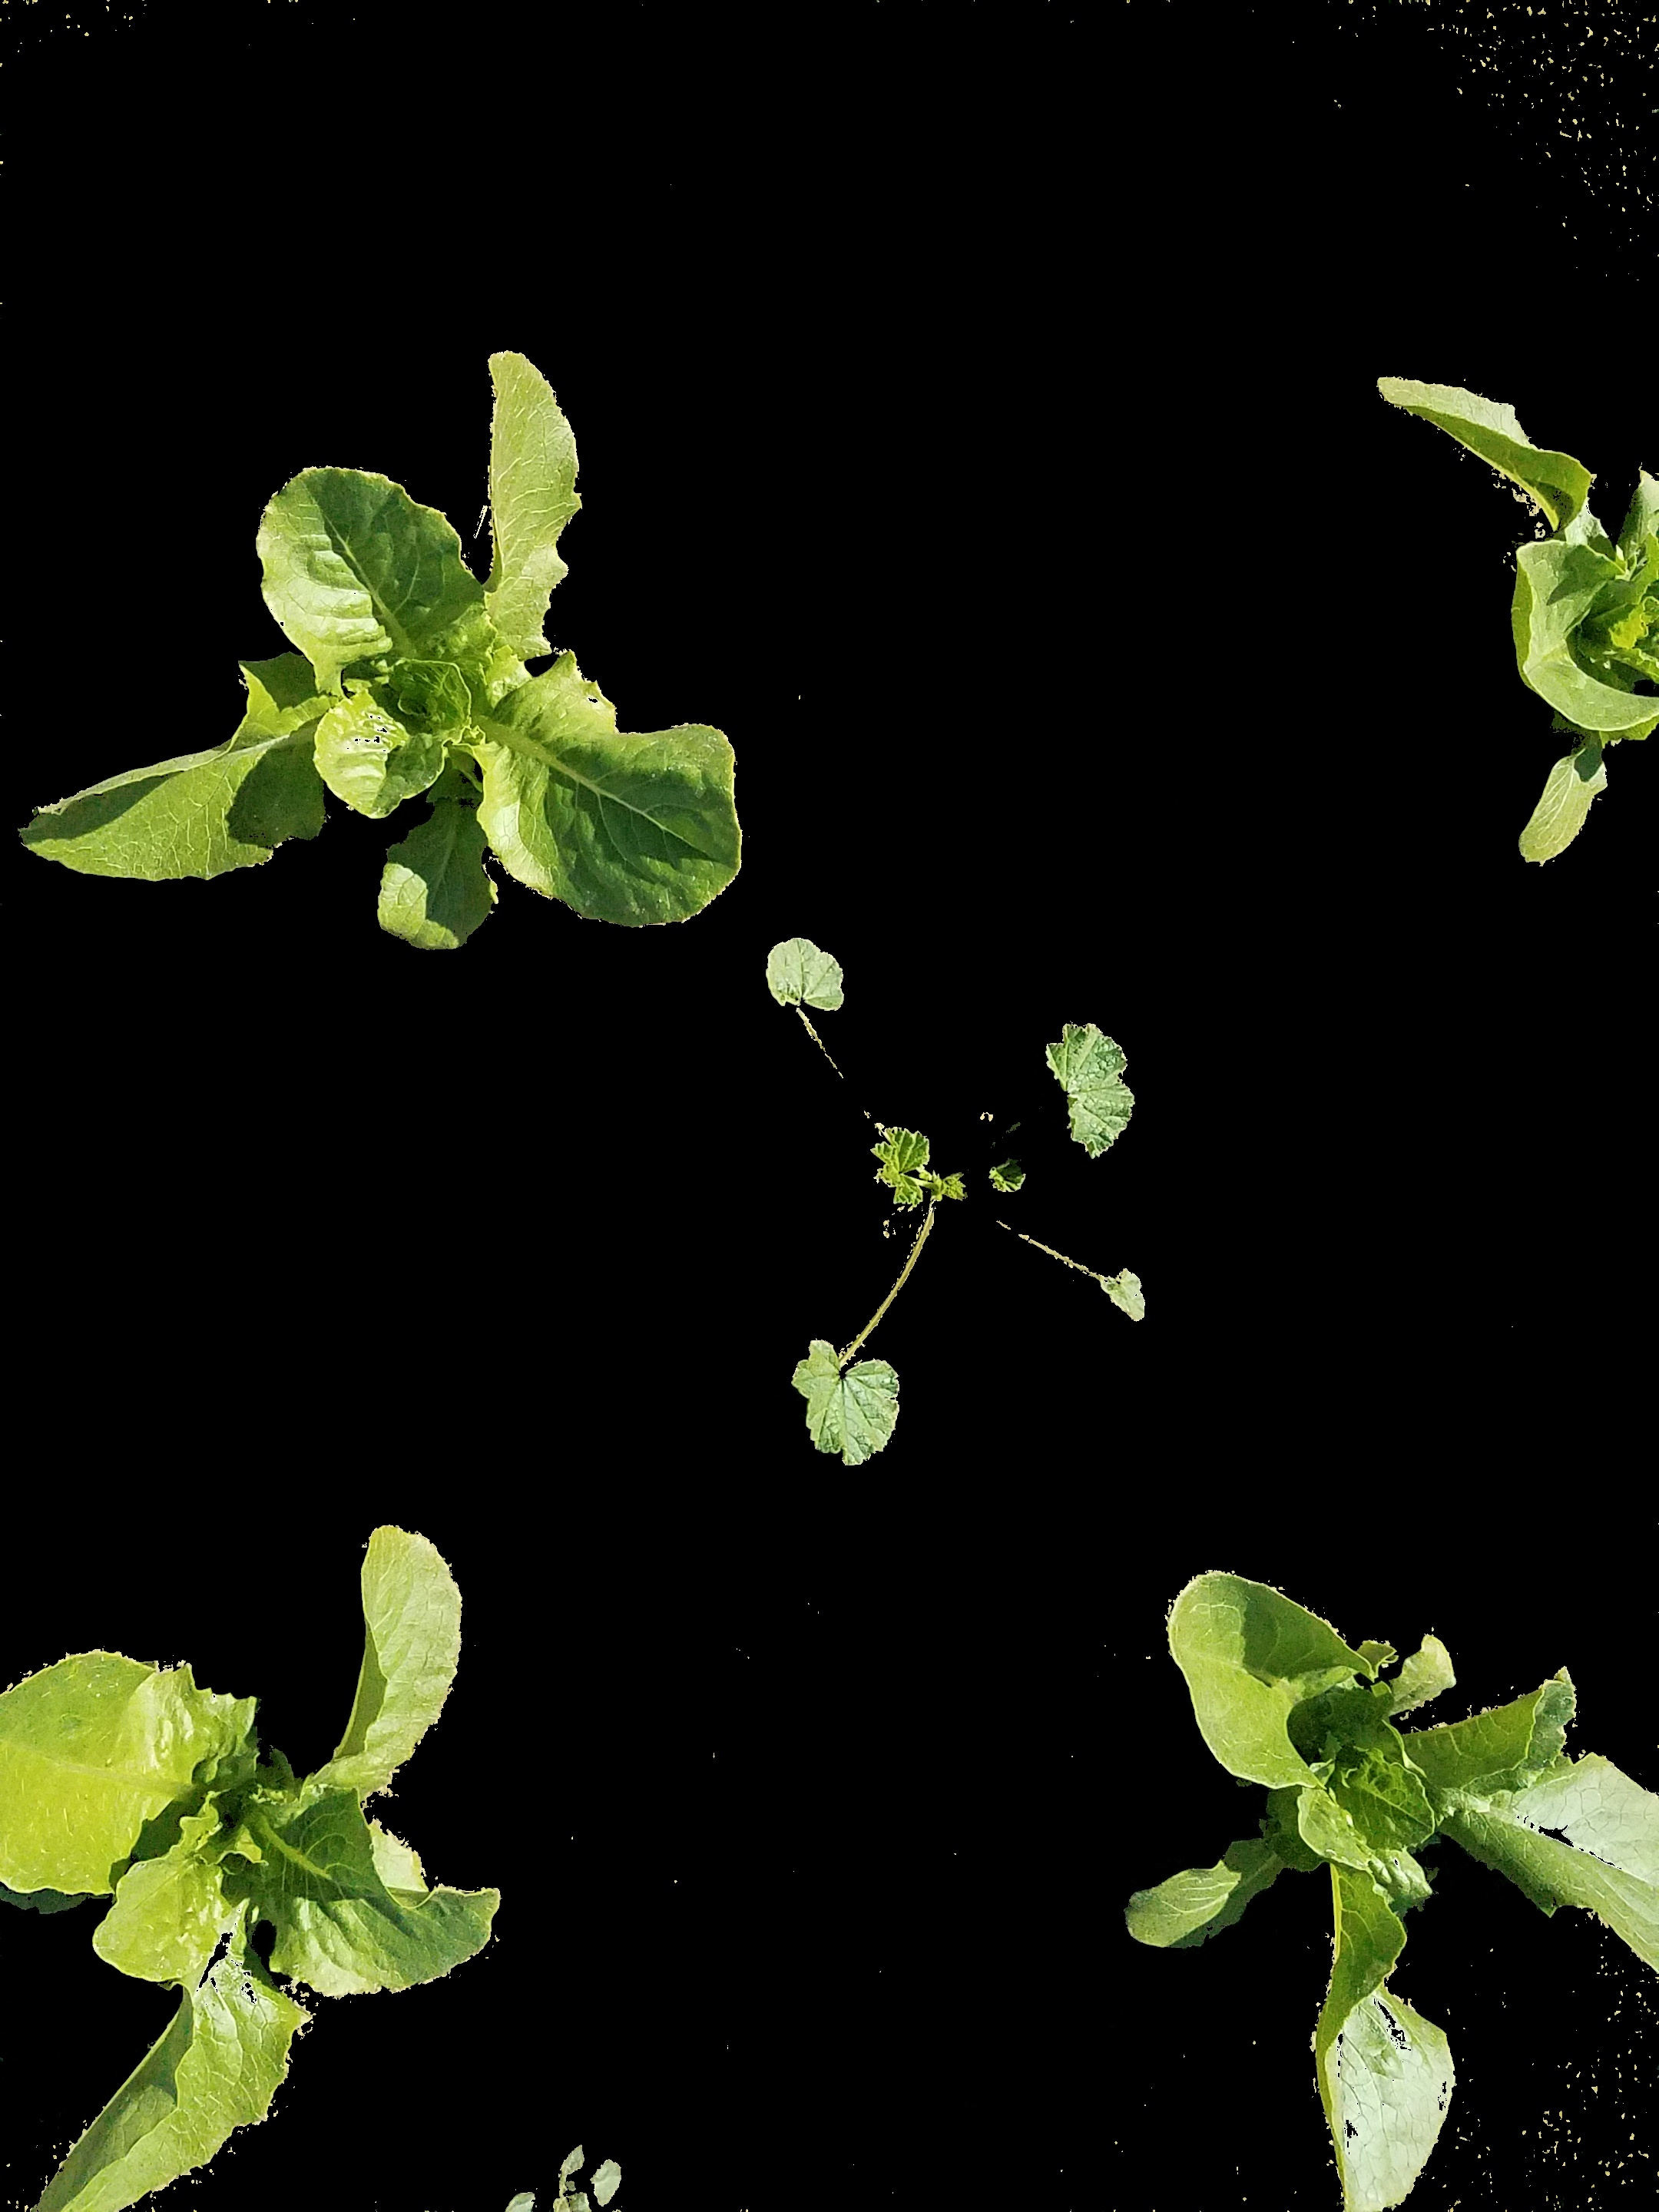
\includegraphics[width =1.25in]{figures/20201117_112624-MexG.jpg} \label{fig:mexg}} \\
\subfloat[TGI]{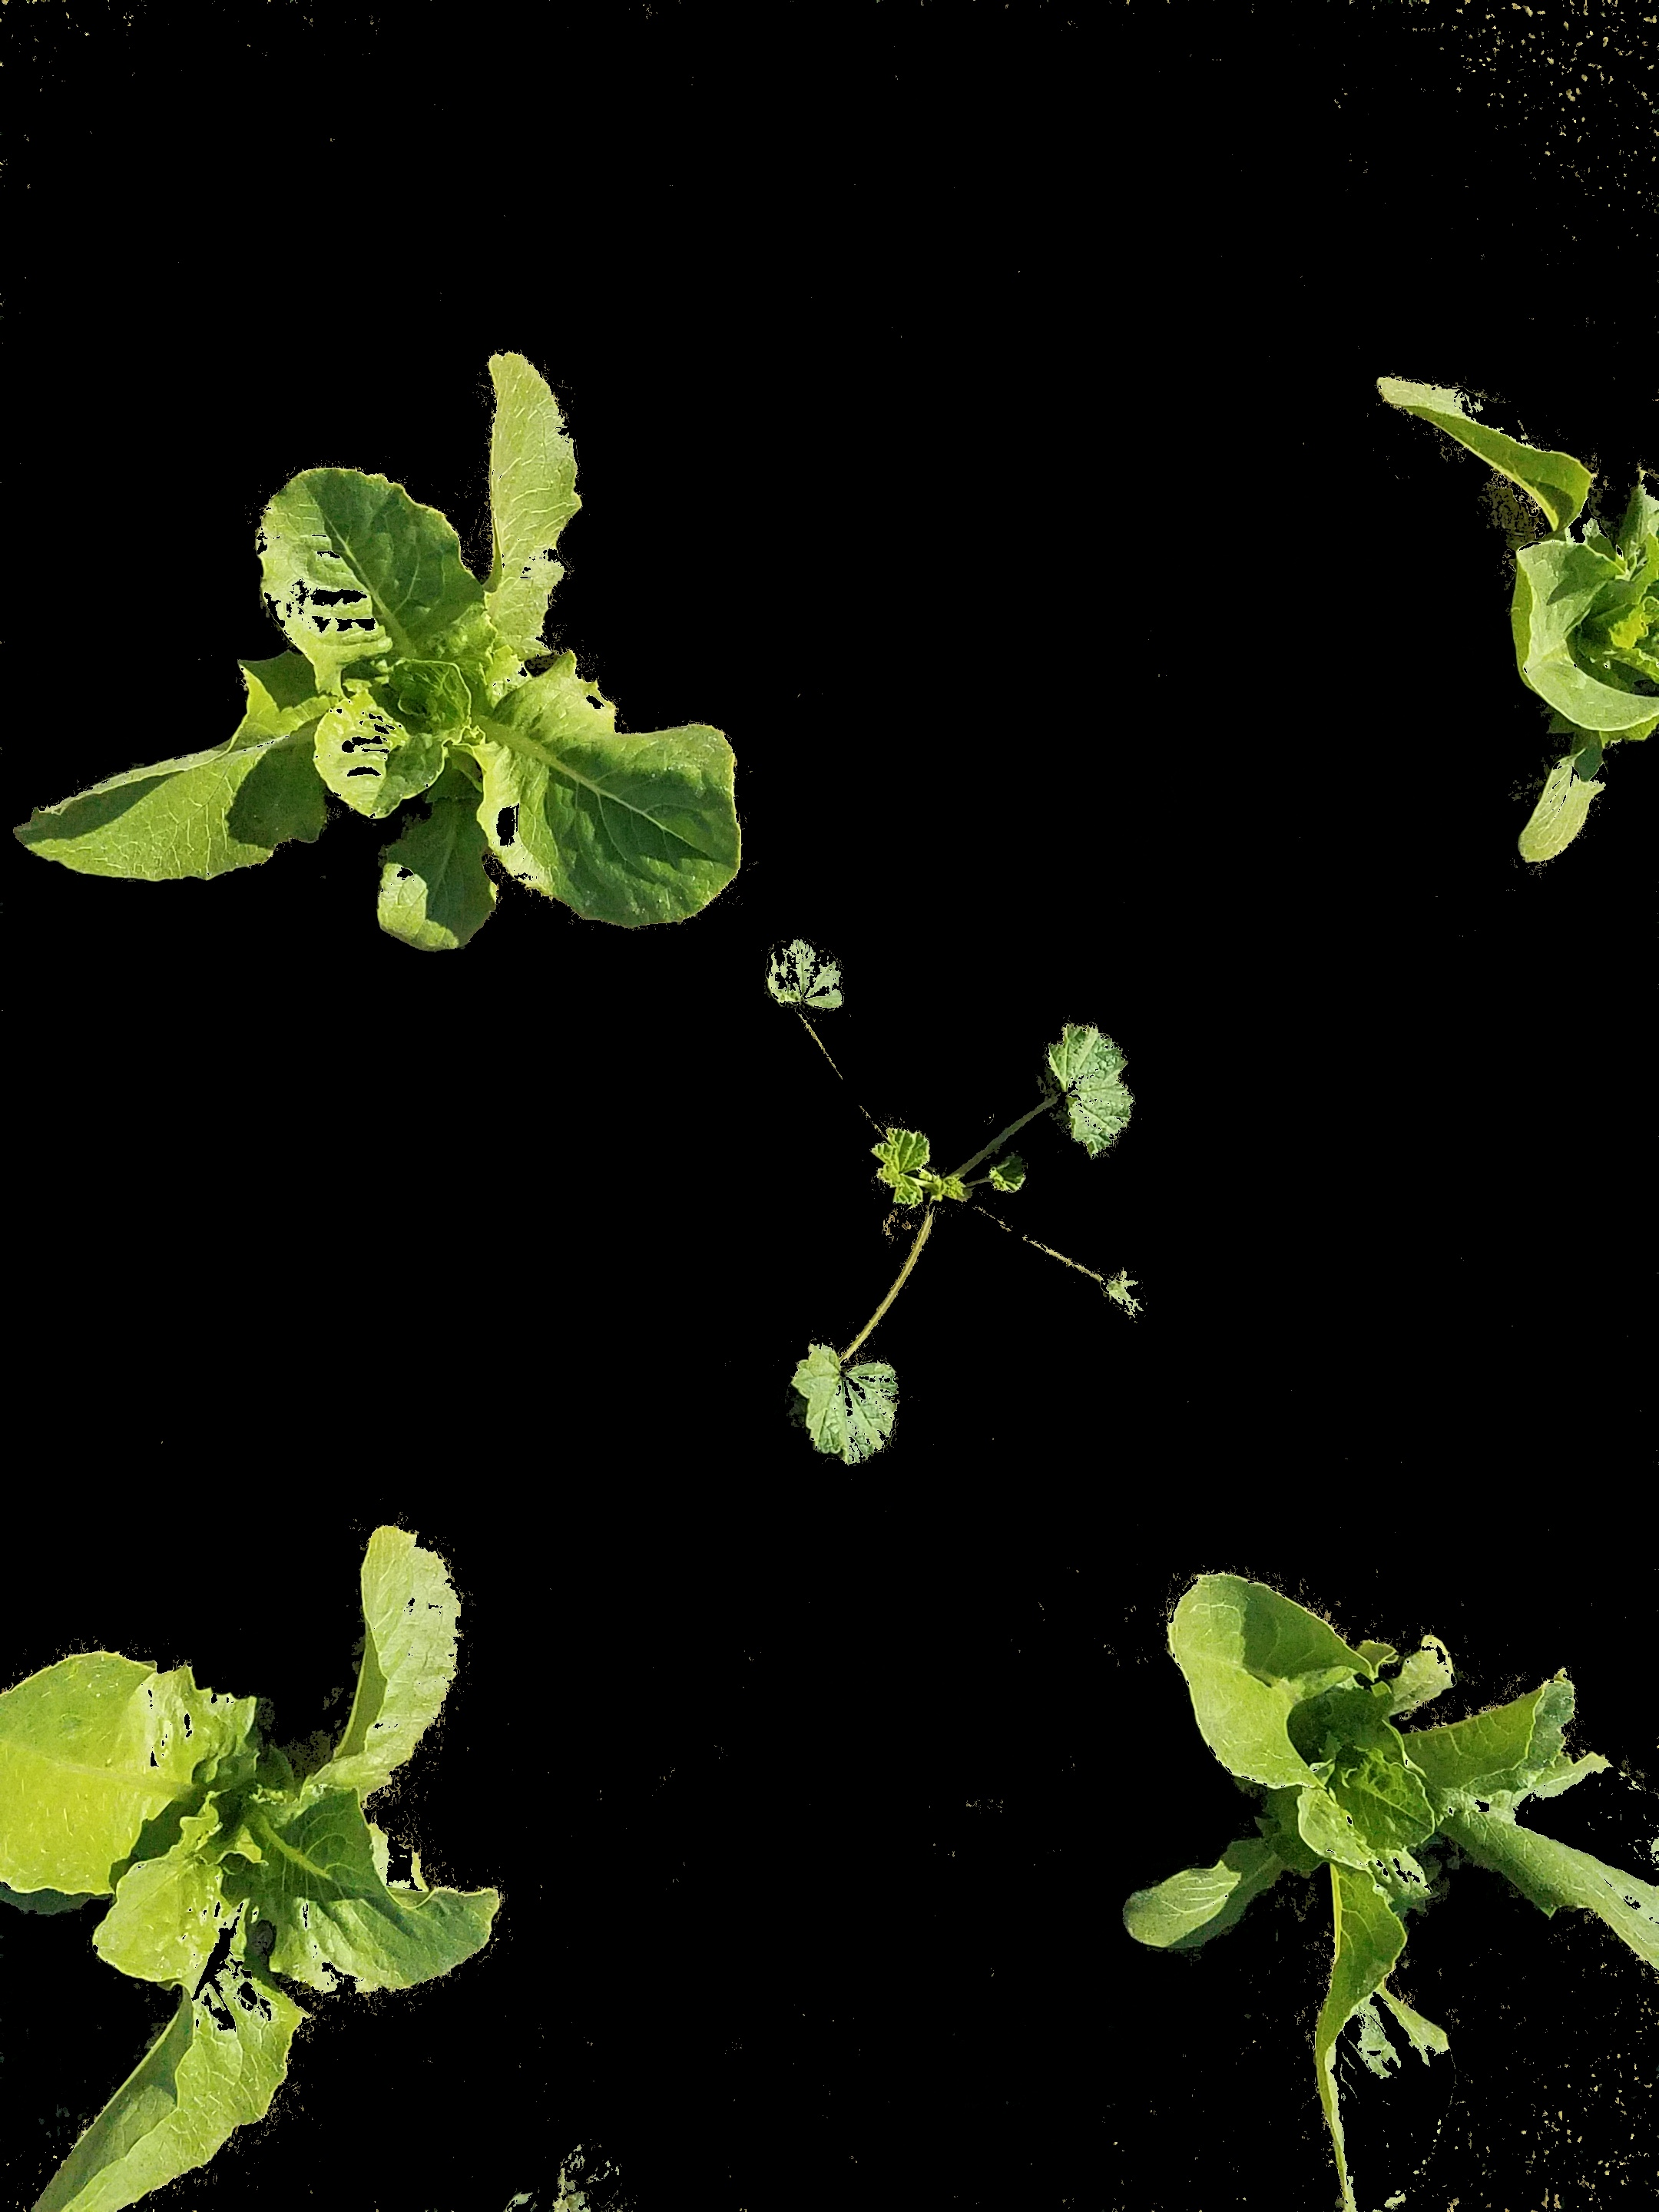
\includegraphics[width =1.25in]{figures/20201117_112624-TGI.jpg} \label{fig:tgi}} &
\subfloat[VEG]{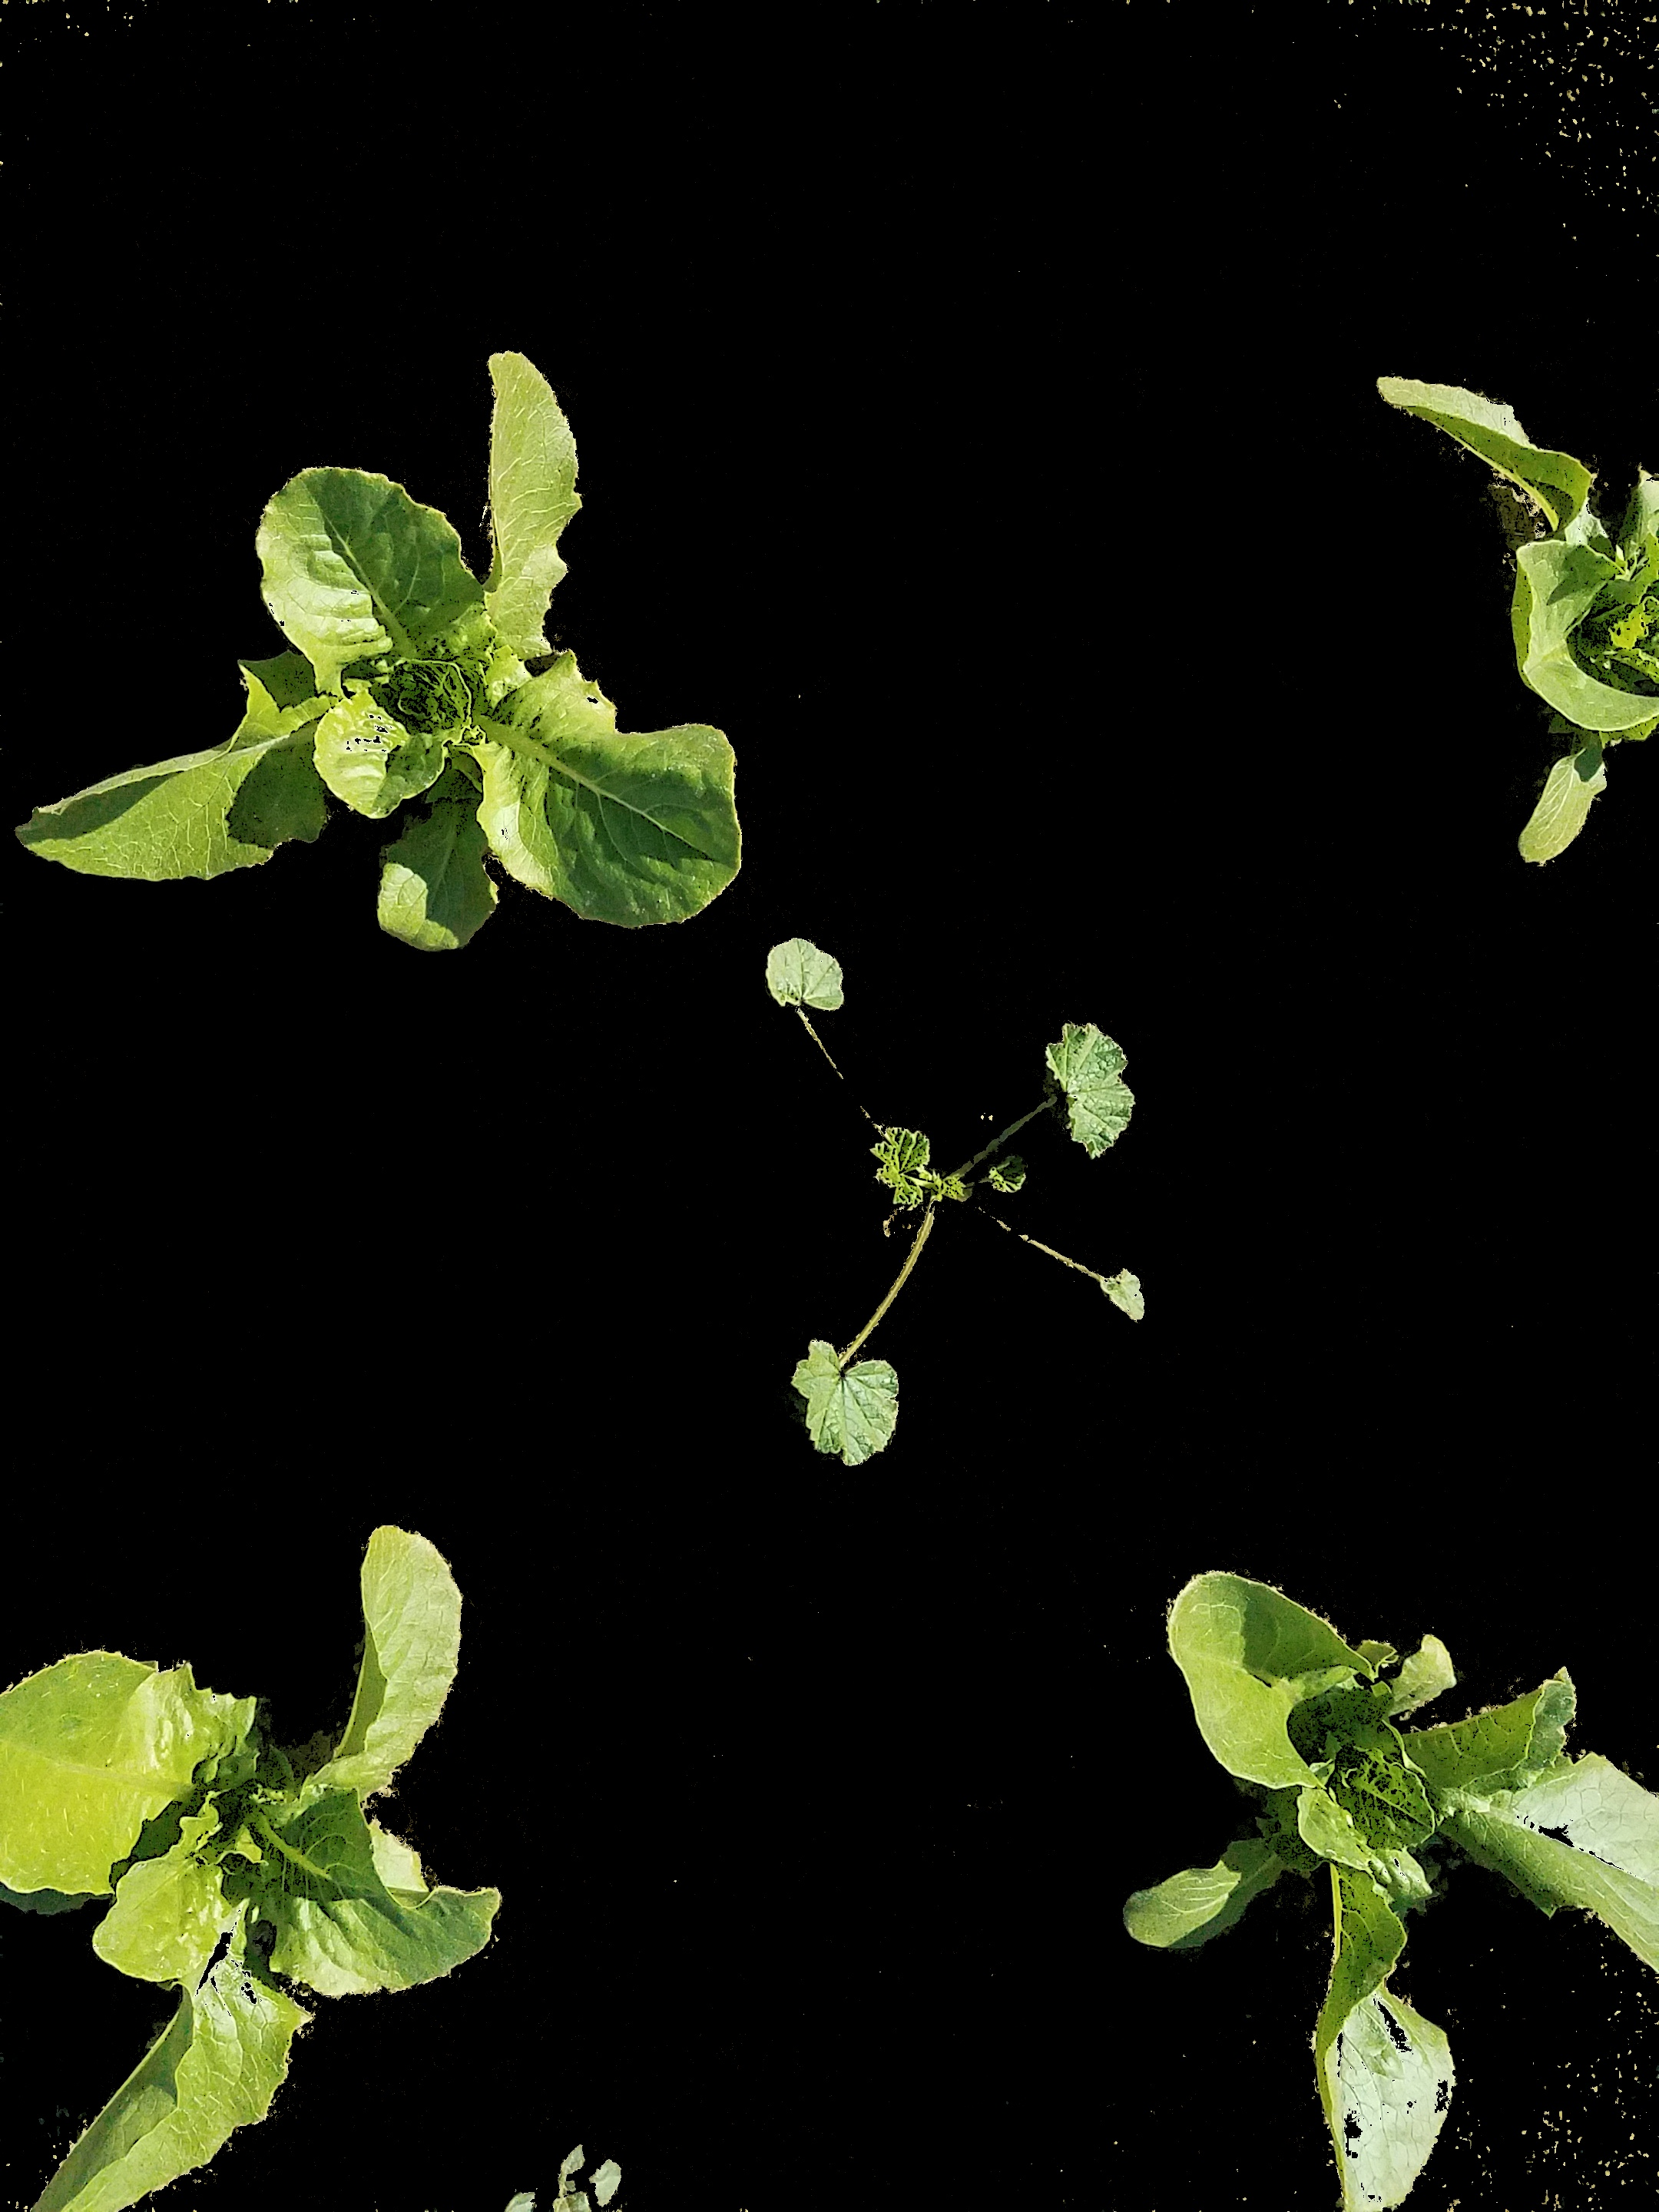
\includegraphics[width =1.25in]{figures/20201117_112624-VEG.jpg} \label{fig:veg}} &
\subfloat[Original]{\includegraphics[scale=0.0415,angle=90]{figures/20201117_112624.jpg} \label{fig:original}} \\

\end{tabular}
\caption[Results of various visible-light image segmentation techniques]{Various visible-light image segmentation techniques (See Table \ref{table:indices} for details). At first glance, many of the segmentation algorithms produce similar results, but some of the methods are not sensitive to less green portions of the plants -- slender stems. Contrast the results seen in \ref{fig:exr} and \ref{fig:mexg}, with the slender stems of the plant in the middle of the image not present in the result of the former.}
\label{figure:results}
\end{figure}

There are two sorts of mistakes encountered in segmentation, as there are only two sorts of things in the image: things that are vegetation (crop and weeds) and things that aren't (typically, the ground). Omission of a crop leaf is apparent in Figure \ref{fig:ndi}, showing the result of using NDI.  The center plant is only partially visible. Contrast that with the result shown in Figures \ref{fig:hi} and  \ref{fig:hv}, where the ground is featured. This case may be due to the shadow of the plant containing too much green as sunlight passes through the leaf. Figure \ref{fig:overlay} illustrates the effects of the index and errors -- of special note here is the error that is shown in the upper right-hand portion of Figure \ref{fig:overlay-cive}. Applying the NDI mask produces the errors discussed previously -- the leaf shadow is identified as vegetation. The evaluation of errors in index-based approaches is illustrated 

\begin{figure}[H]
	\centering
	\subfloat[CIVE mask overlay\centering]{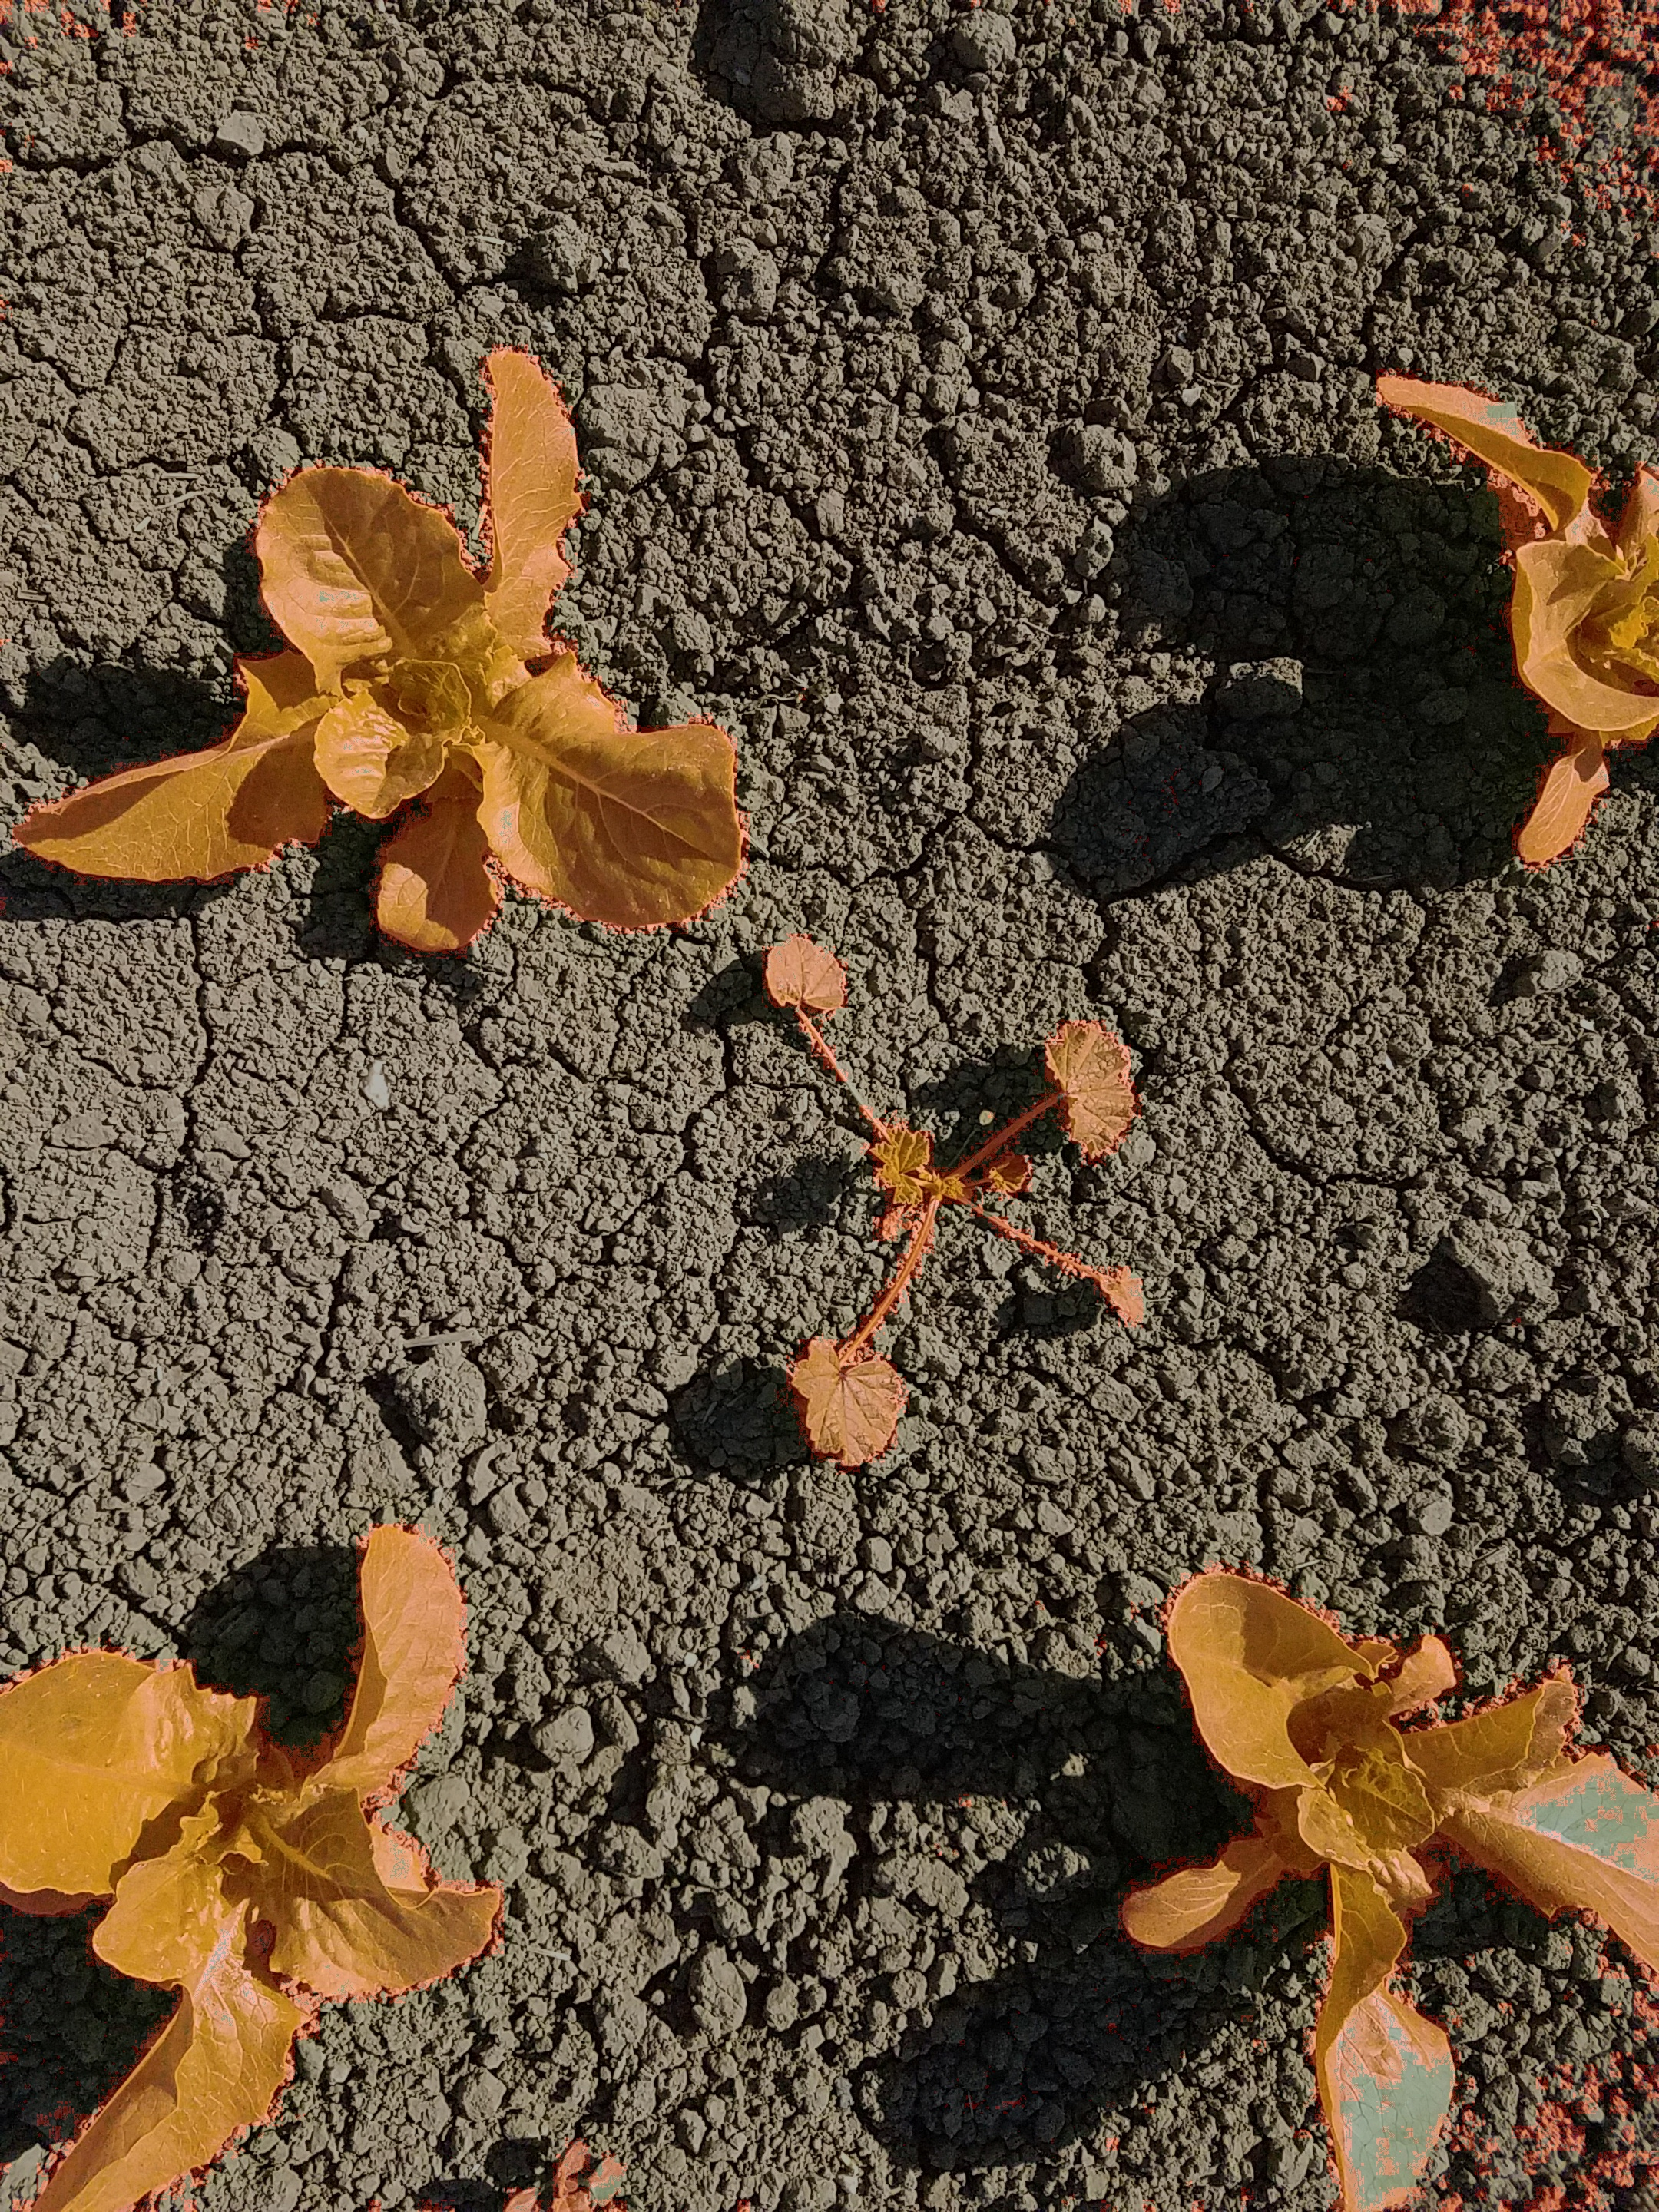
\includegraphics[width=0.45\textwidth]{figures/overlay-cive.jpg}\label{fig:overlay-cive}}
	\hfill
	\subfloat[NDI mask overlay\centering]{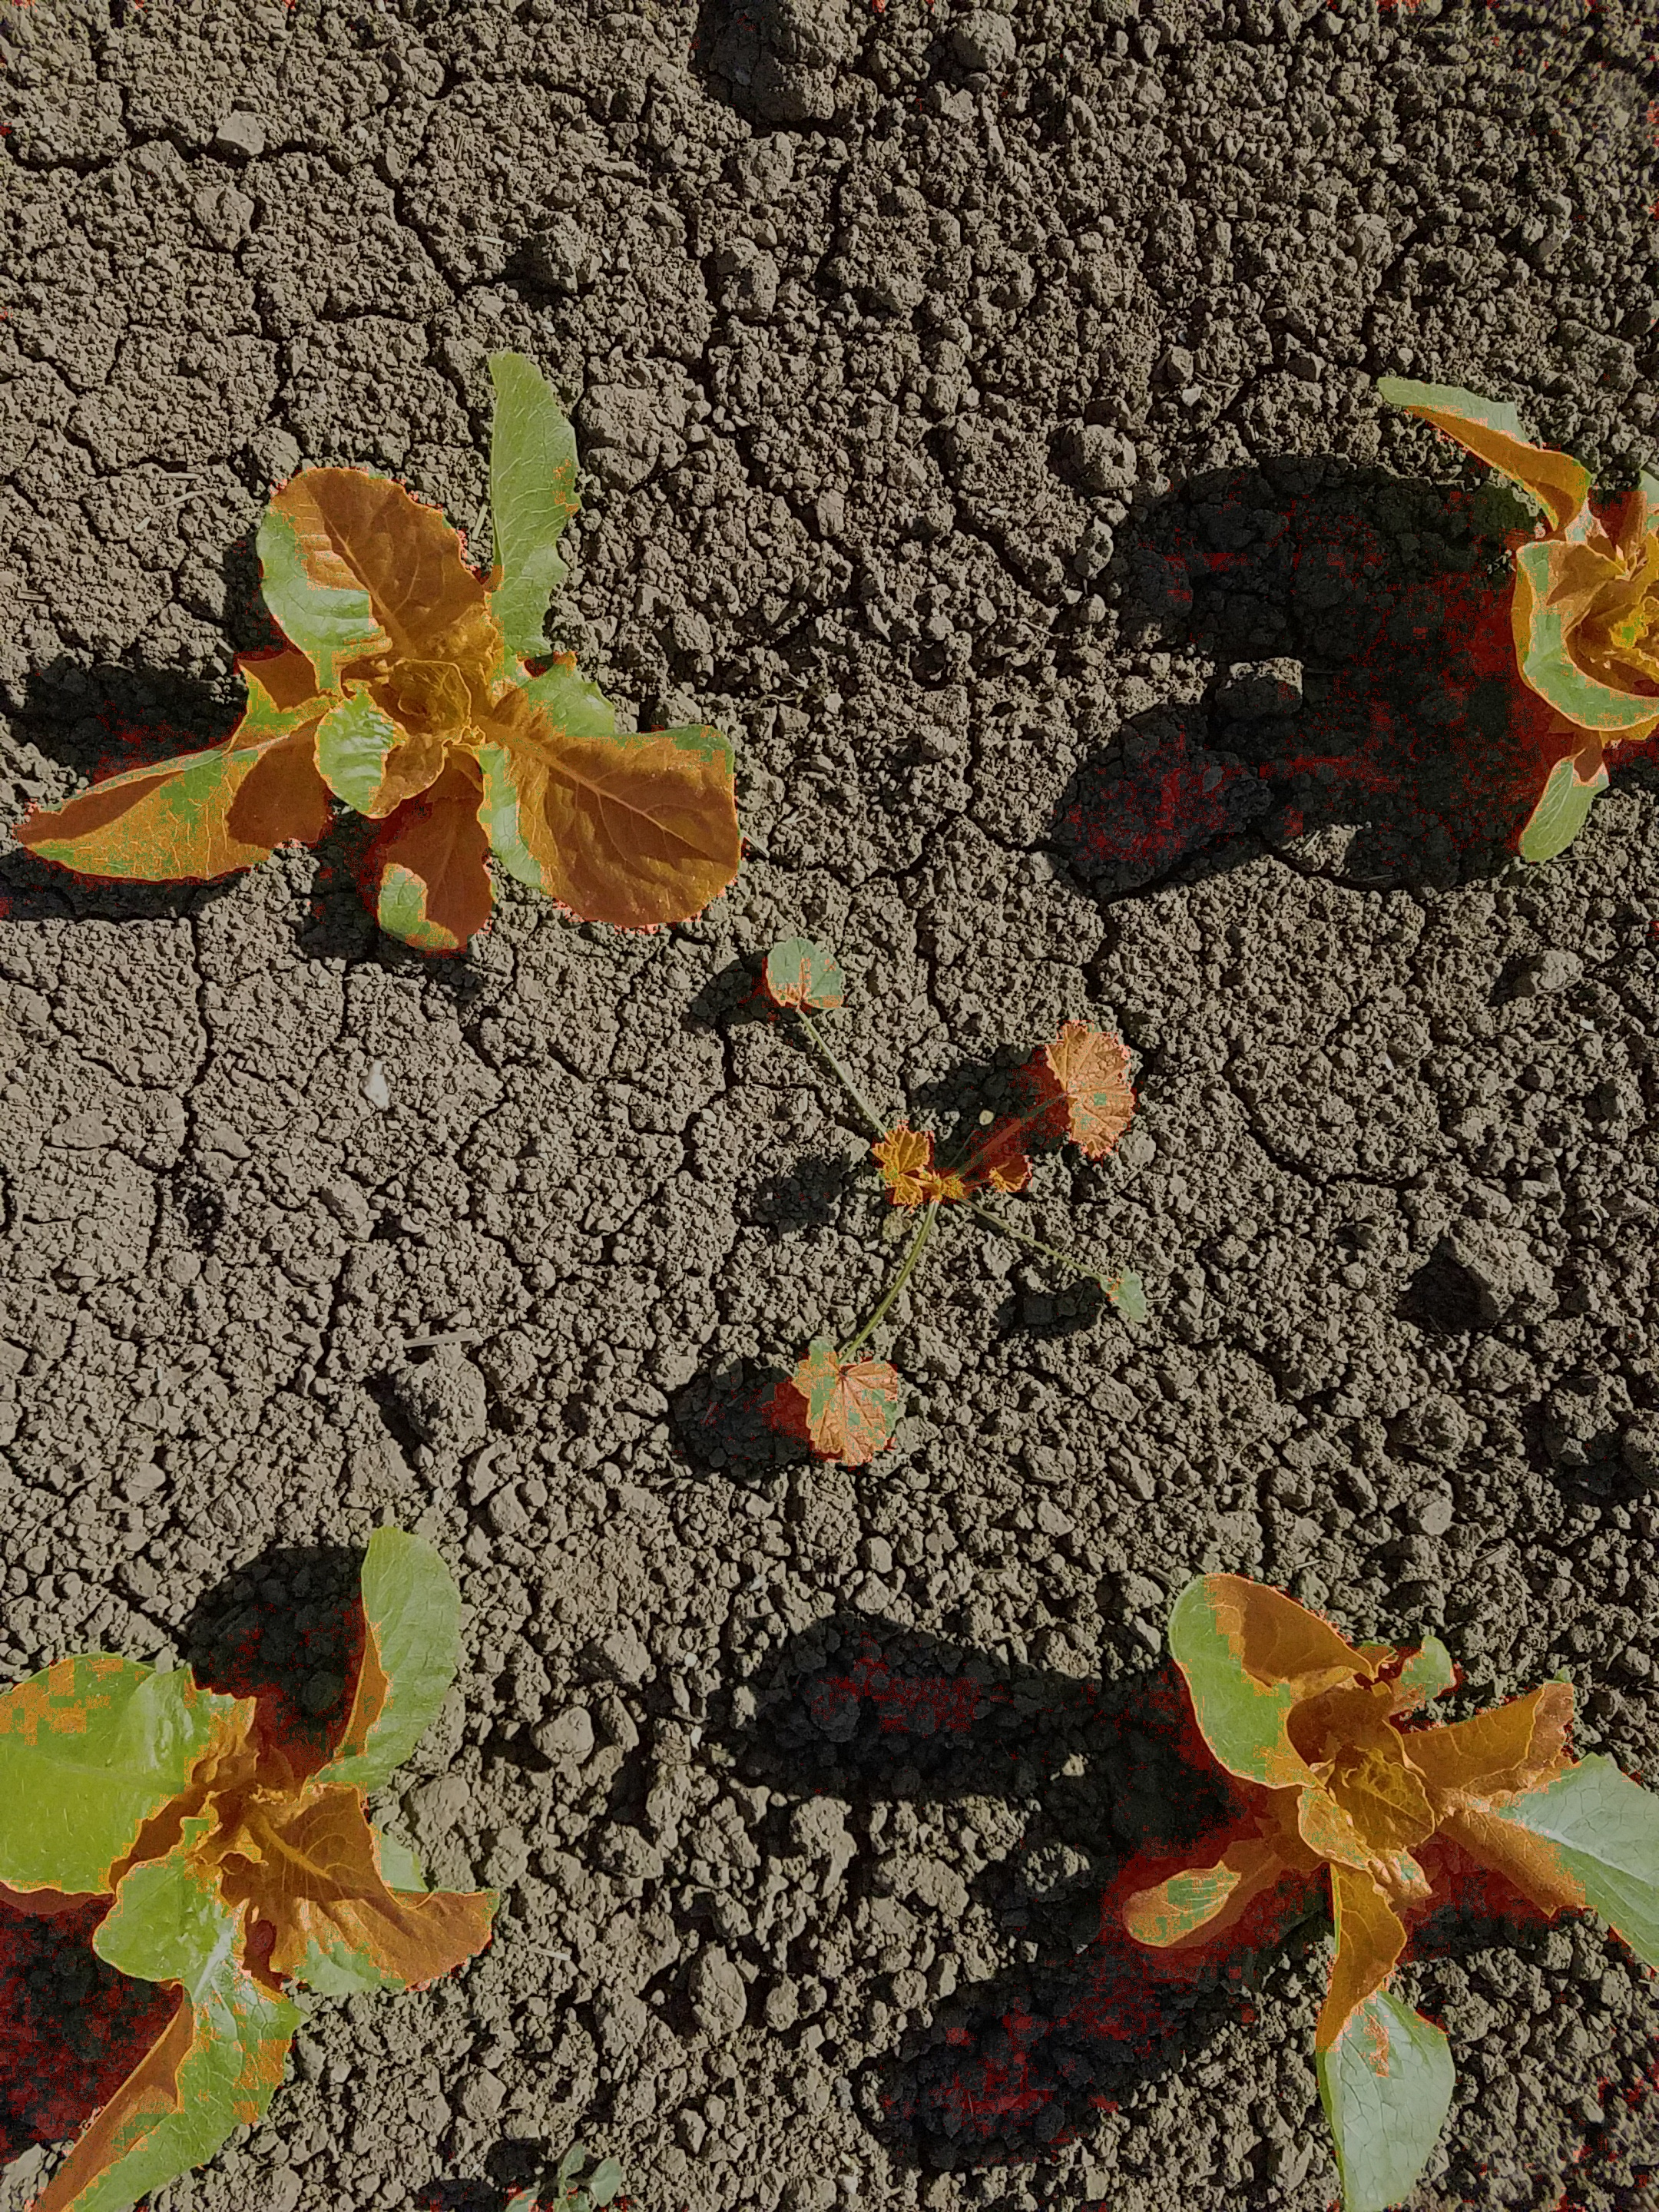
\includegraphics[width=0.45\textwidth]{figures/overlay-ndi.jpg}\label{fig:overlay-ndi}}
	\caption[Masks overlayed on original images]{Masks produced with CIVE and NDI overlayed on the original image. In these images, the masks used are colored red and blended with the original image. Areas that are tinted red will be shown, so a `correct' mask will completely cover vegetation. Note the mask shown in \ref{fig:overlay-ndi} does not cover the plant completely, and segments out shadow portions of the image. What seems to be going on here is that sunlight is shining through the leaf, making the ground green enough to be interpreted as vegetation. Contrast this with the errors seen in \ref{fig:overlay-cive}, where portions of the ground are incorrectly segmented as vegetation in cases not attributable to color contamination. (The upper right-hand portion of \ref{fig:overlay-cive} is a good example of this error.) Photo: Dr. Mark Seimens, University of Arizona.}
	\label{fig:overlay}
\end{figure}

\subsubsection{HSI and HSV}
The Hue, Saturation and Intensity (HSI) and Hue Saturation and Value (HSV) color spaces present an opportunity to consider how saturated the colors are instead of just emphasizing the green found it an image. While that is a bit of an over-simplification of basing a technique on the values found within the RGB bands, it is essentially what is happening. Hue based approaches take much the same approach in one respect -- the hue frequently present in vegetation (green) is represented as peaking around $120^o$ in both models. This is convenient, certainly, as simply considering points as vegetation of they contain hue values around the peak. How wide this range is, of course, will determine what is captured. And while the topic of color is revisited in Section ~\ref{section:problems-color}, consider that leaves contain much that is not green, just as the ground contains much that is not brown. A leaf may contain hue values in the range of 40-70, an indication that the hue is toward the red end of the representation. Likewise, a patch of dirt may contain hue values in the range of 15-20, an indication that the hue is much more red than anything else. HSV is a bit more complicated, in that the V band should be normalized between $(0..1)$ and mutiplied by the H value. Lacking more creative terms, these indices will be referred to as HI and HV. 

\begin{equation}
	\label{equation:hsi}
	HSI
    \begin{split}
		discard~pixels~with~H~channel &\geq 190~or \leq 55\\
		discard~pixels~with~S~channel &\leq 0.45 \\
		discard~pixels~with~I~band &\geq 50
    \end{split}
\end{equation}

\begin{equation}
	\label{equation:hsv}
	HSV
	\begin{split}
		H * norm(V) \\
	\end{split}
\end{equation}

\subsubsection{CIELAB}
The CIELAB color space, often referred to with L*A*B* in the name, expresses color along three lines: Lightness (L), Green-Red (A), and Blue-Yellow (B). These values seen in these bands have different ranges, L ranging from 0 (black) to 100 (white), A ranging from negative (green) to positive (red), and B ranging from negative (blue) to positive (yellow). The A and B bands are not technically limited to a specific range, as this space was designed to exceed human perception. Human perception of these colors can be covered with a $\pm 150$ range, and implementations tend to limit the values reported in these bands for pragmatic reasons.  For the purposes of indexing vegetation the bands of  most interest are the A and B bands. Taking the difference between B and A and discarding pixels with a difference is below 30 yields acceptable results. This index will be referred to as CI throughout this document.

\begin{equation}
		\label{equation:cielab}
		B - A, discard~results~\leq~30
\end{equation}

\subsubsection{YCbCr}
This color space (sometimes termed YCC) is frequently encountered in video transmission, as it is designed to address the redundancies seen in the RGB color space. It uses the $Y$ channel to carry Luma information (black and white) and two color channels expressing the blue difference (Cb) and red difference (Cr). Separating the brightness from the color components allows the color representations to match human perception -- as our eyes are more sensitive to changes in brightness than they are to color. As with other indices, the objective is to exaggerate the band vegetation occupies and ignoring components that are not. Using equation \ref{equation:ycbcr} achieves that goal.
\begin{equation}
	\label{equation:ycbcr}
	\ln(Cr) * Cb, discard\ results\geq 890
\end{equation}
This index will be referred to as YCbCRI throughout this document.
\subsubsection{YIQ}
The YIQ model of color was used by the (analog) NTSC color TV system. Later, digital transmission schemes used different color spaces, notably the YCbCr that will be addressed in more detail in a separate section. These schemes have a common approach: \textit{chrominance} (a color component) is added to a black and white image. In the YIQ model, $Y$ represents the luma information (black and white), with $I$ (in-phase, representing red-cyan contrast) and $Q$ (quadature, representing magenta-green contrast) the chrominance information. 
The processing employed here is to convert the image to the YIQ color space and take the mean value for the $I$, or in-phase component for the blob's pixels. (\cite{MathWorks_undated-jg}) For segmentation purposes, the information in the Q band is helpful, primarily in discarding things that are not vegetation.
\begin{equation}
	\label{equation:yiq}
	discard\ any\ pixel\ with\ Q\ band\leq 0.04
\end{equation}
This index will be referred to as YI throughout this document.

\begin{figure}[H]
\centering
\begin{tabular}{ccc}
	\subfloat[CIElab]{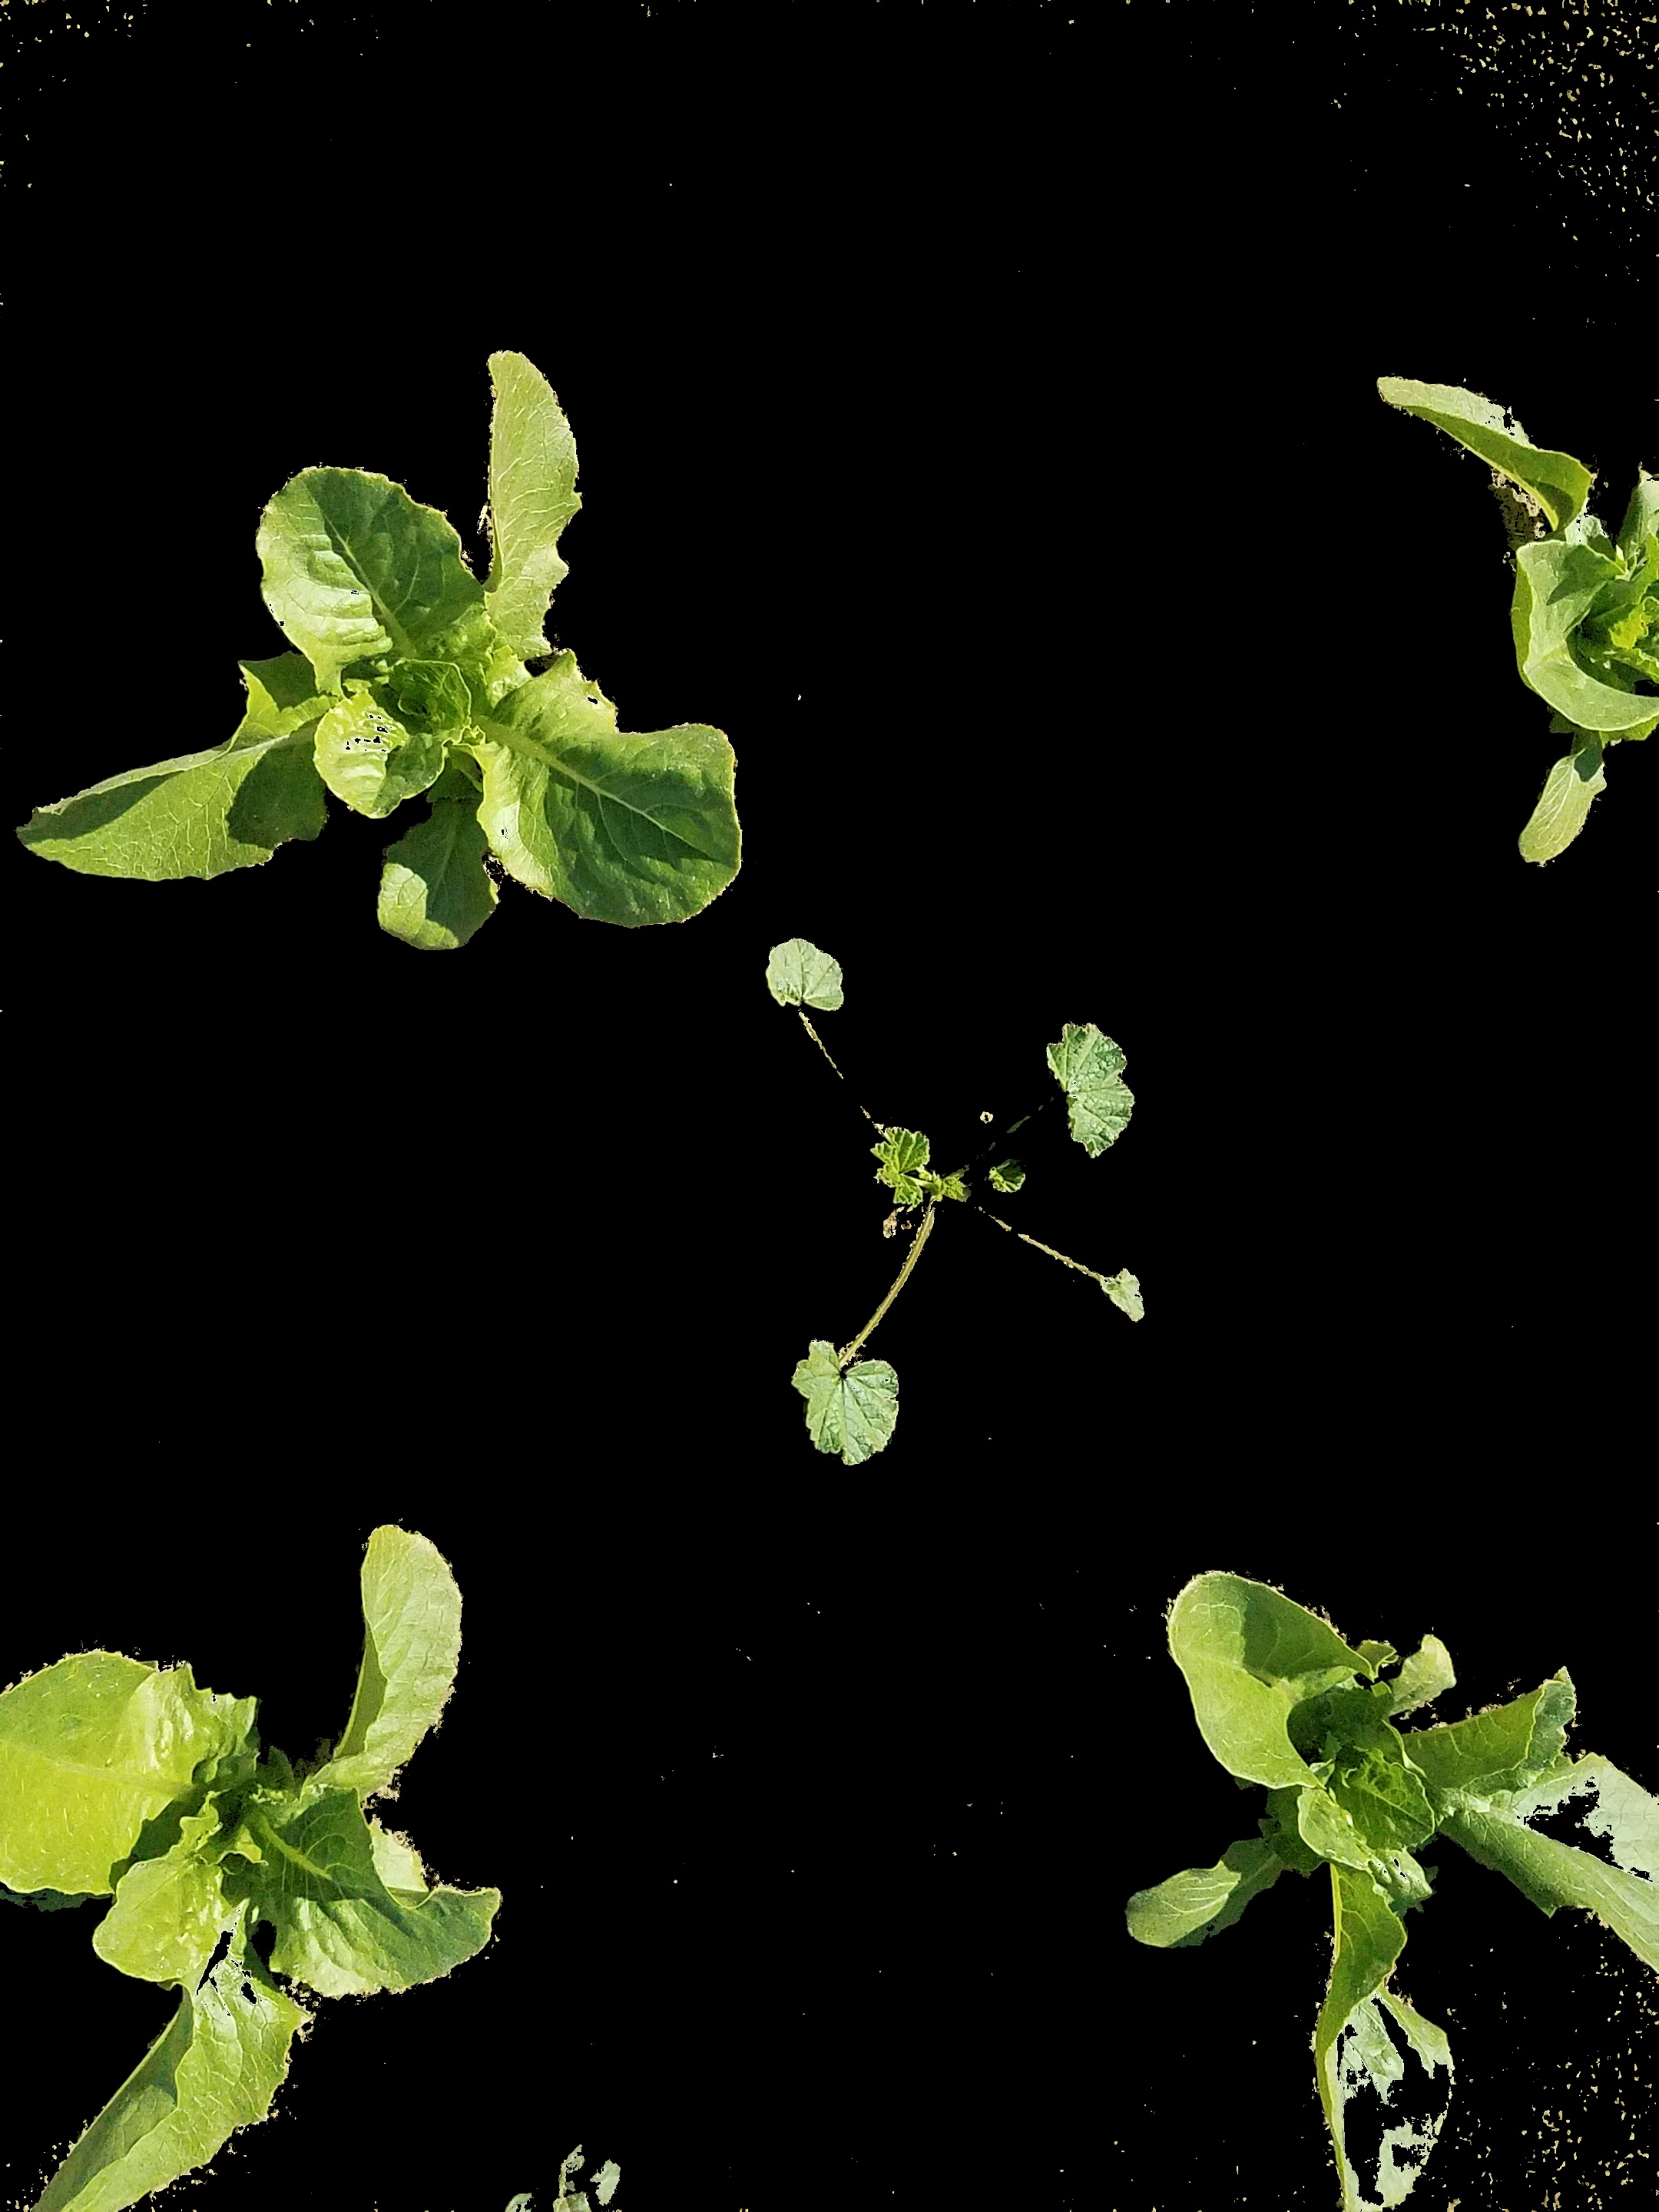
\includegraphics[width = 1.25in]{figures/20201117_112624-CI.jpg} \label{fig:ci}} &
	\subfloat[HSI]{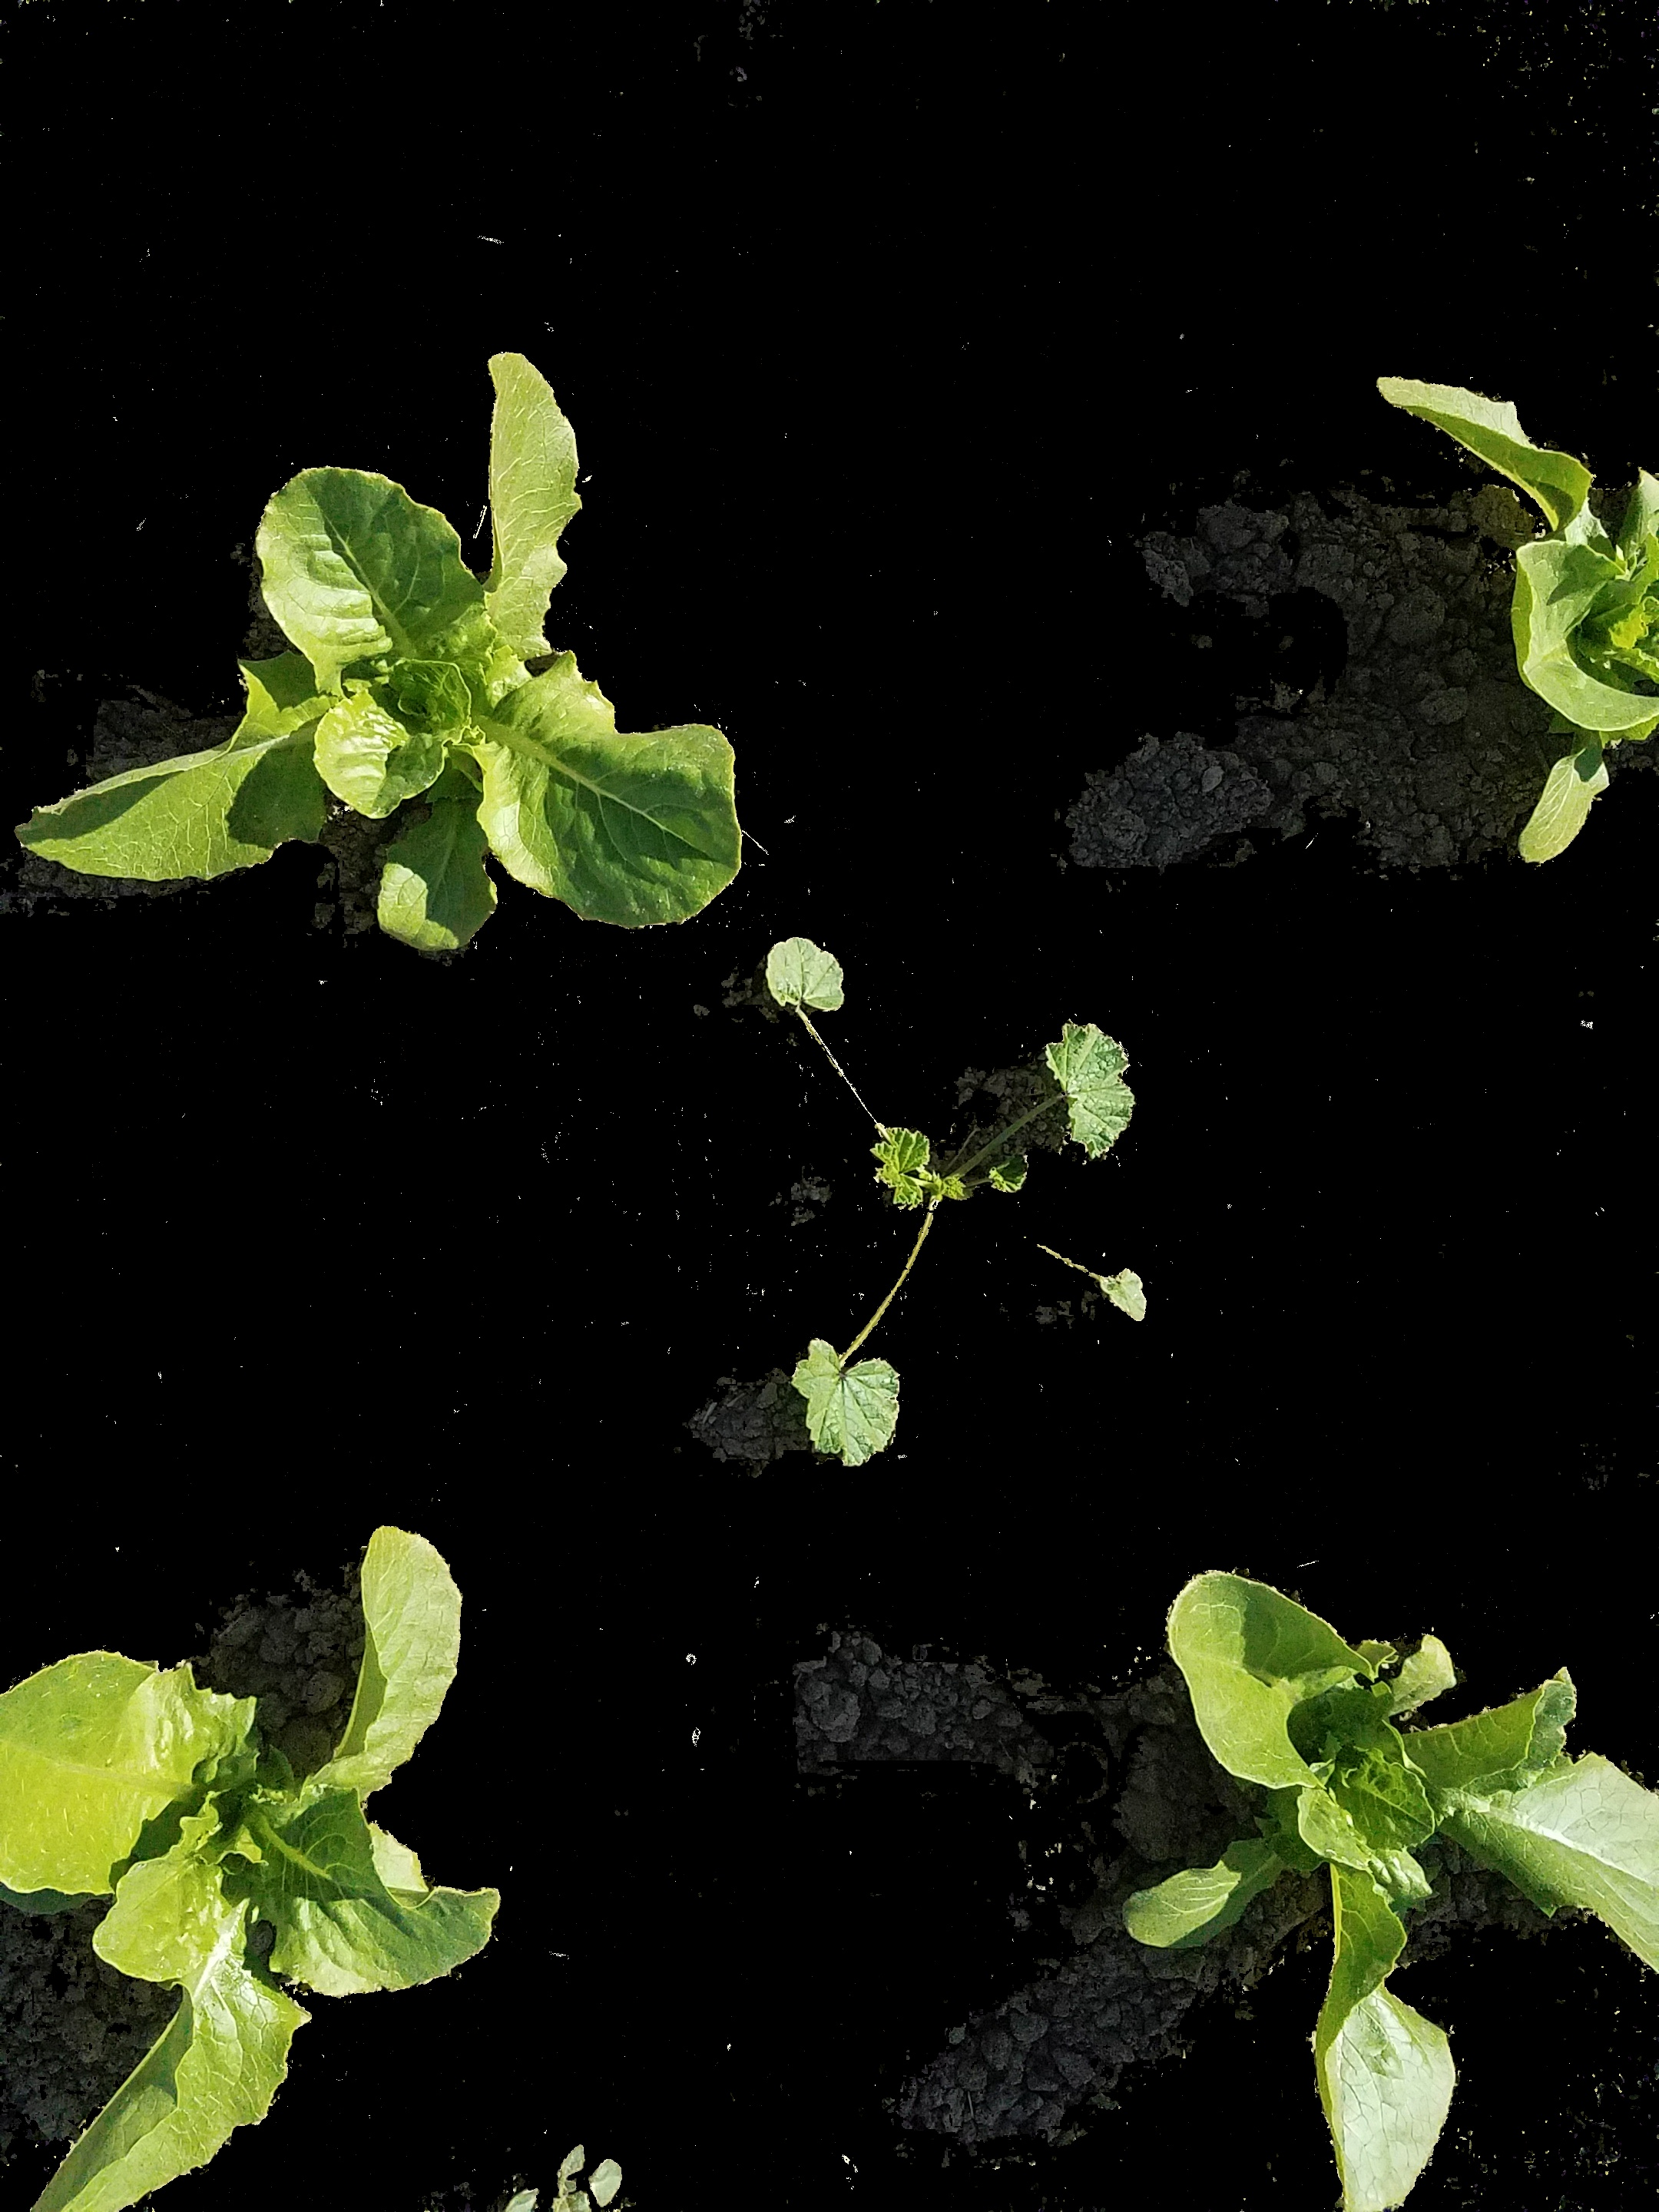
\includegraphics[width = 1.25in]{figures/20201117_112624-HI.jpg} \label{fig:hi}} &
	\subfloat[HSV]{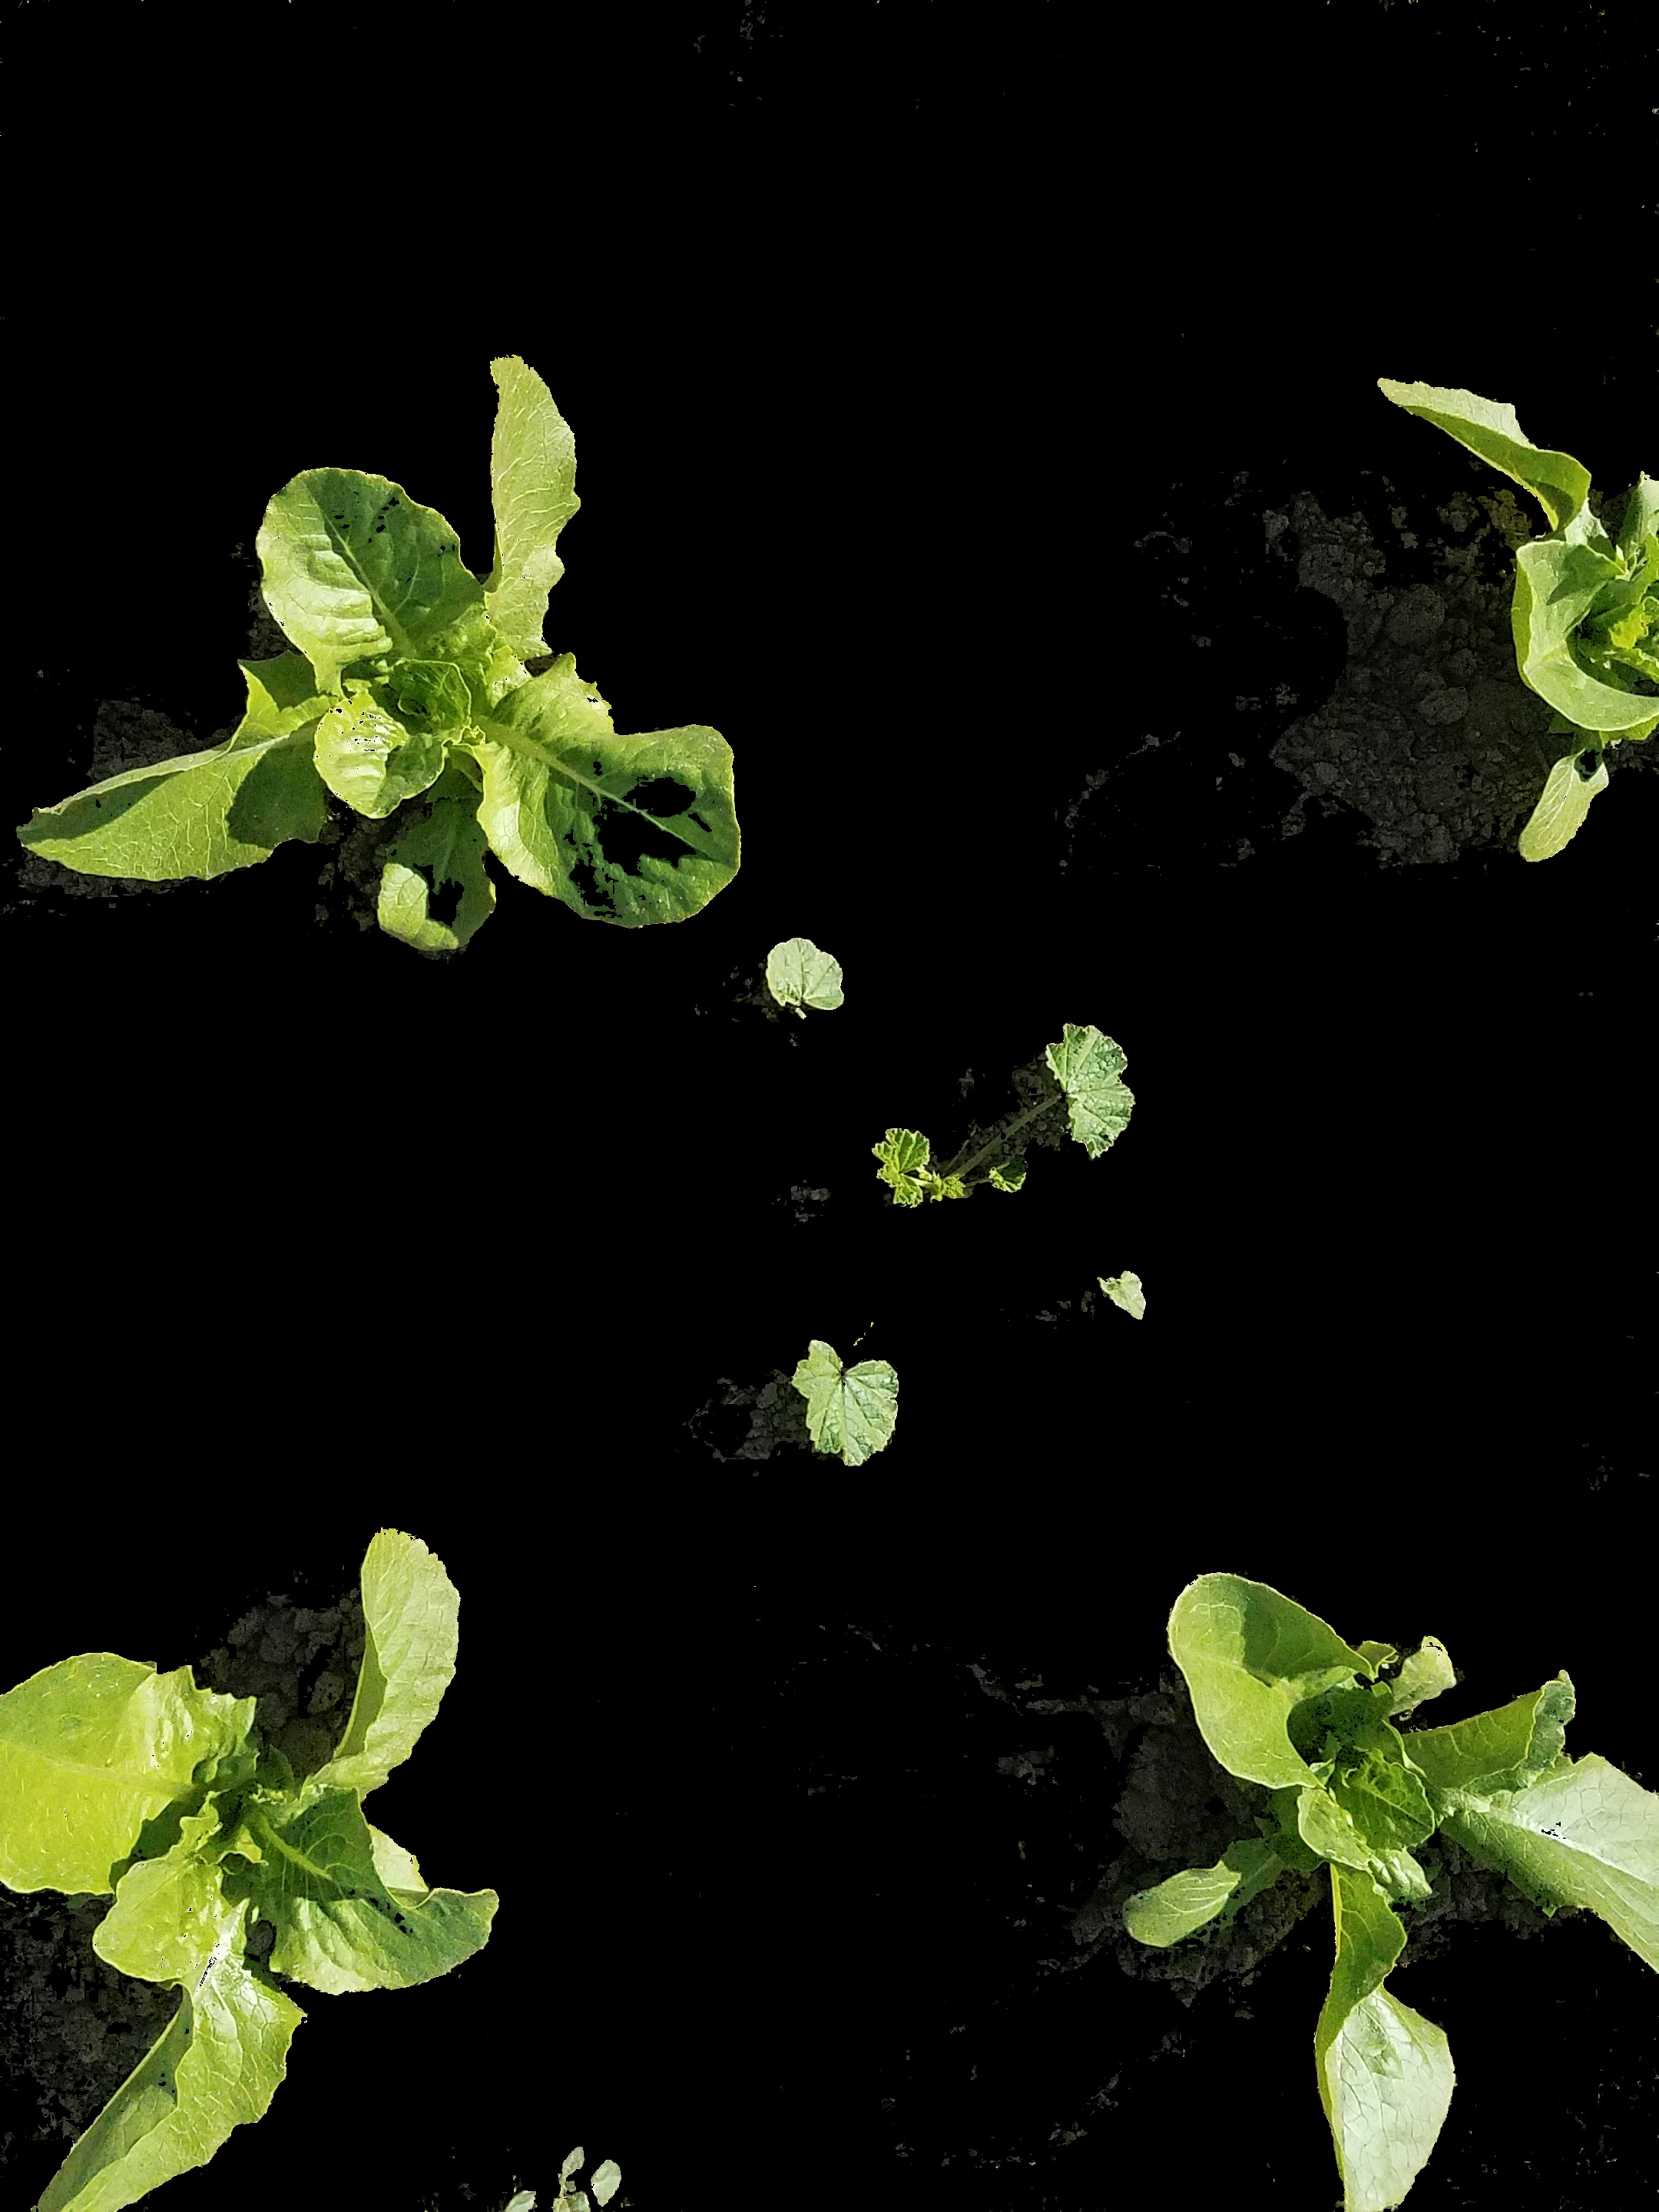
\includegraphics[width = 1.25in]{figures/20201117_112624-HV.jpg} \label{fig:hv}} \\
	\subfloat[YCbCr]{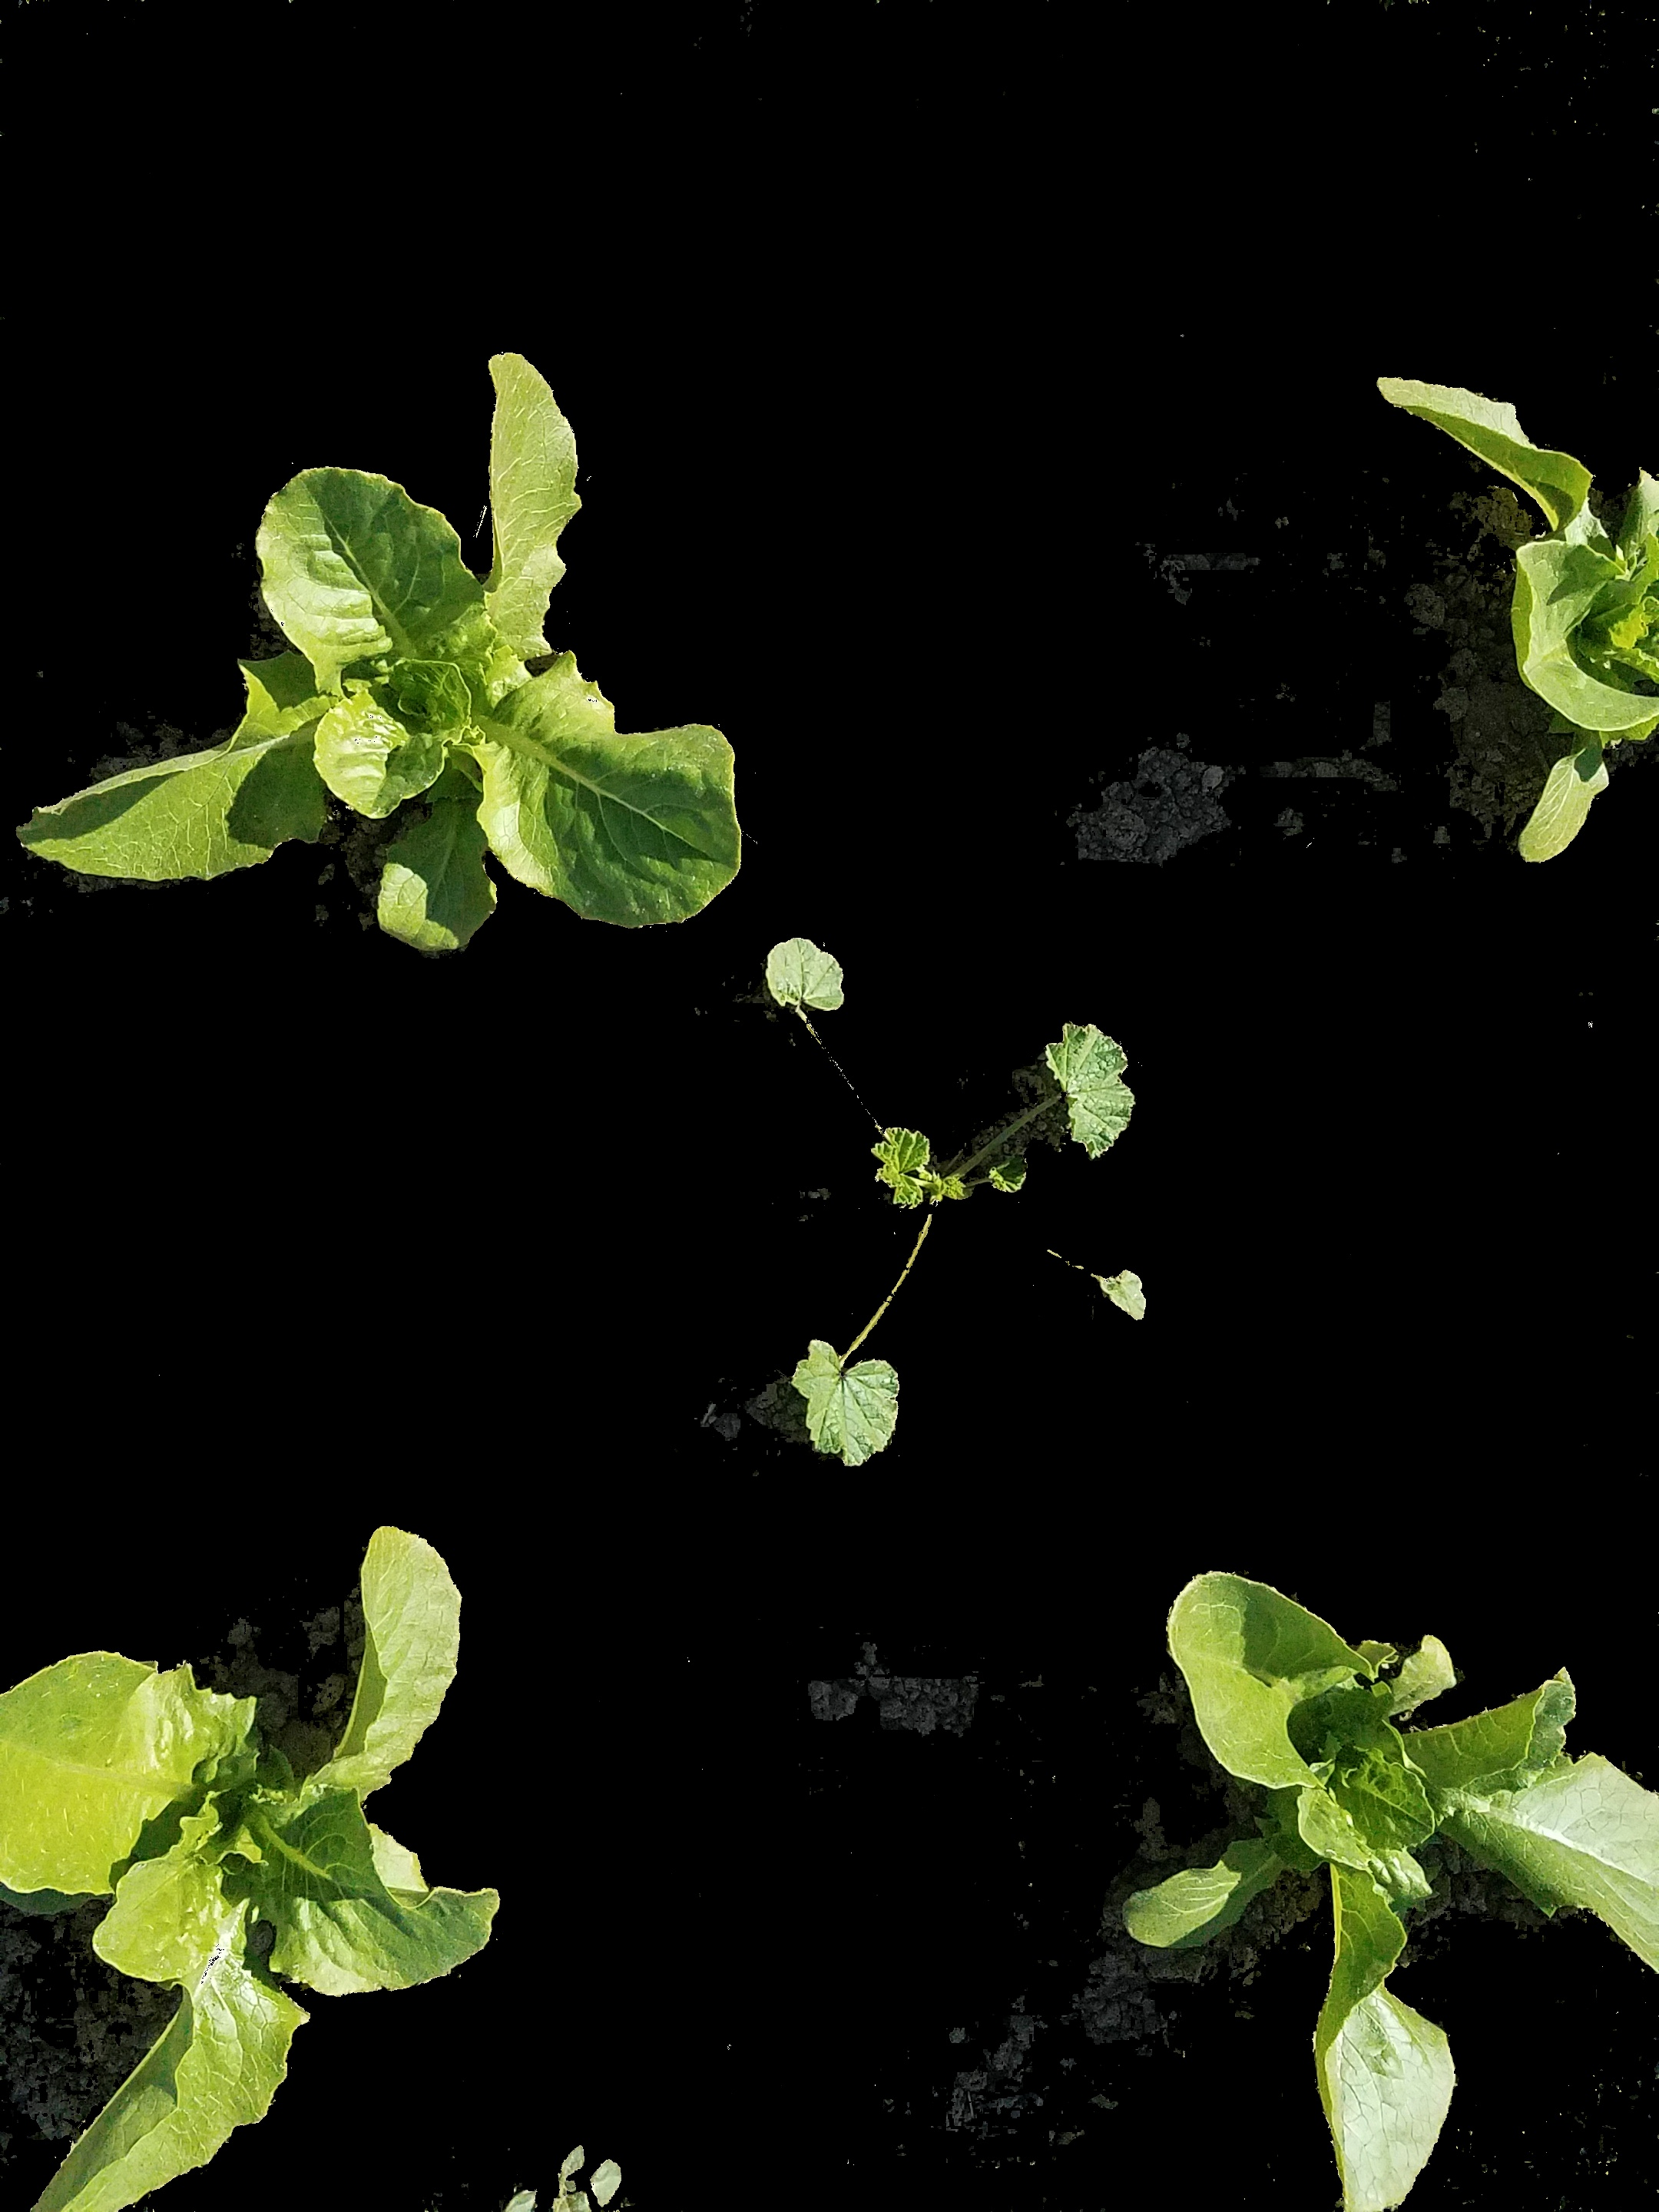
\includegraphics[width = 1.25in]{figures/20201117_112624-YCbCrI.jpg} \label{fig:ycbcr}} &
	\subfloat[YIQ]{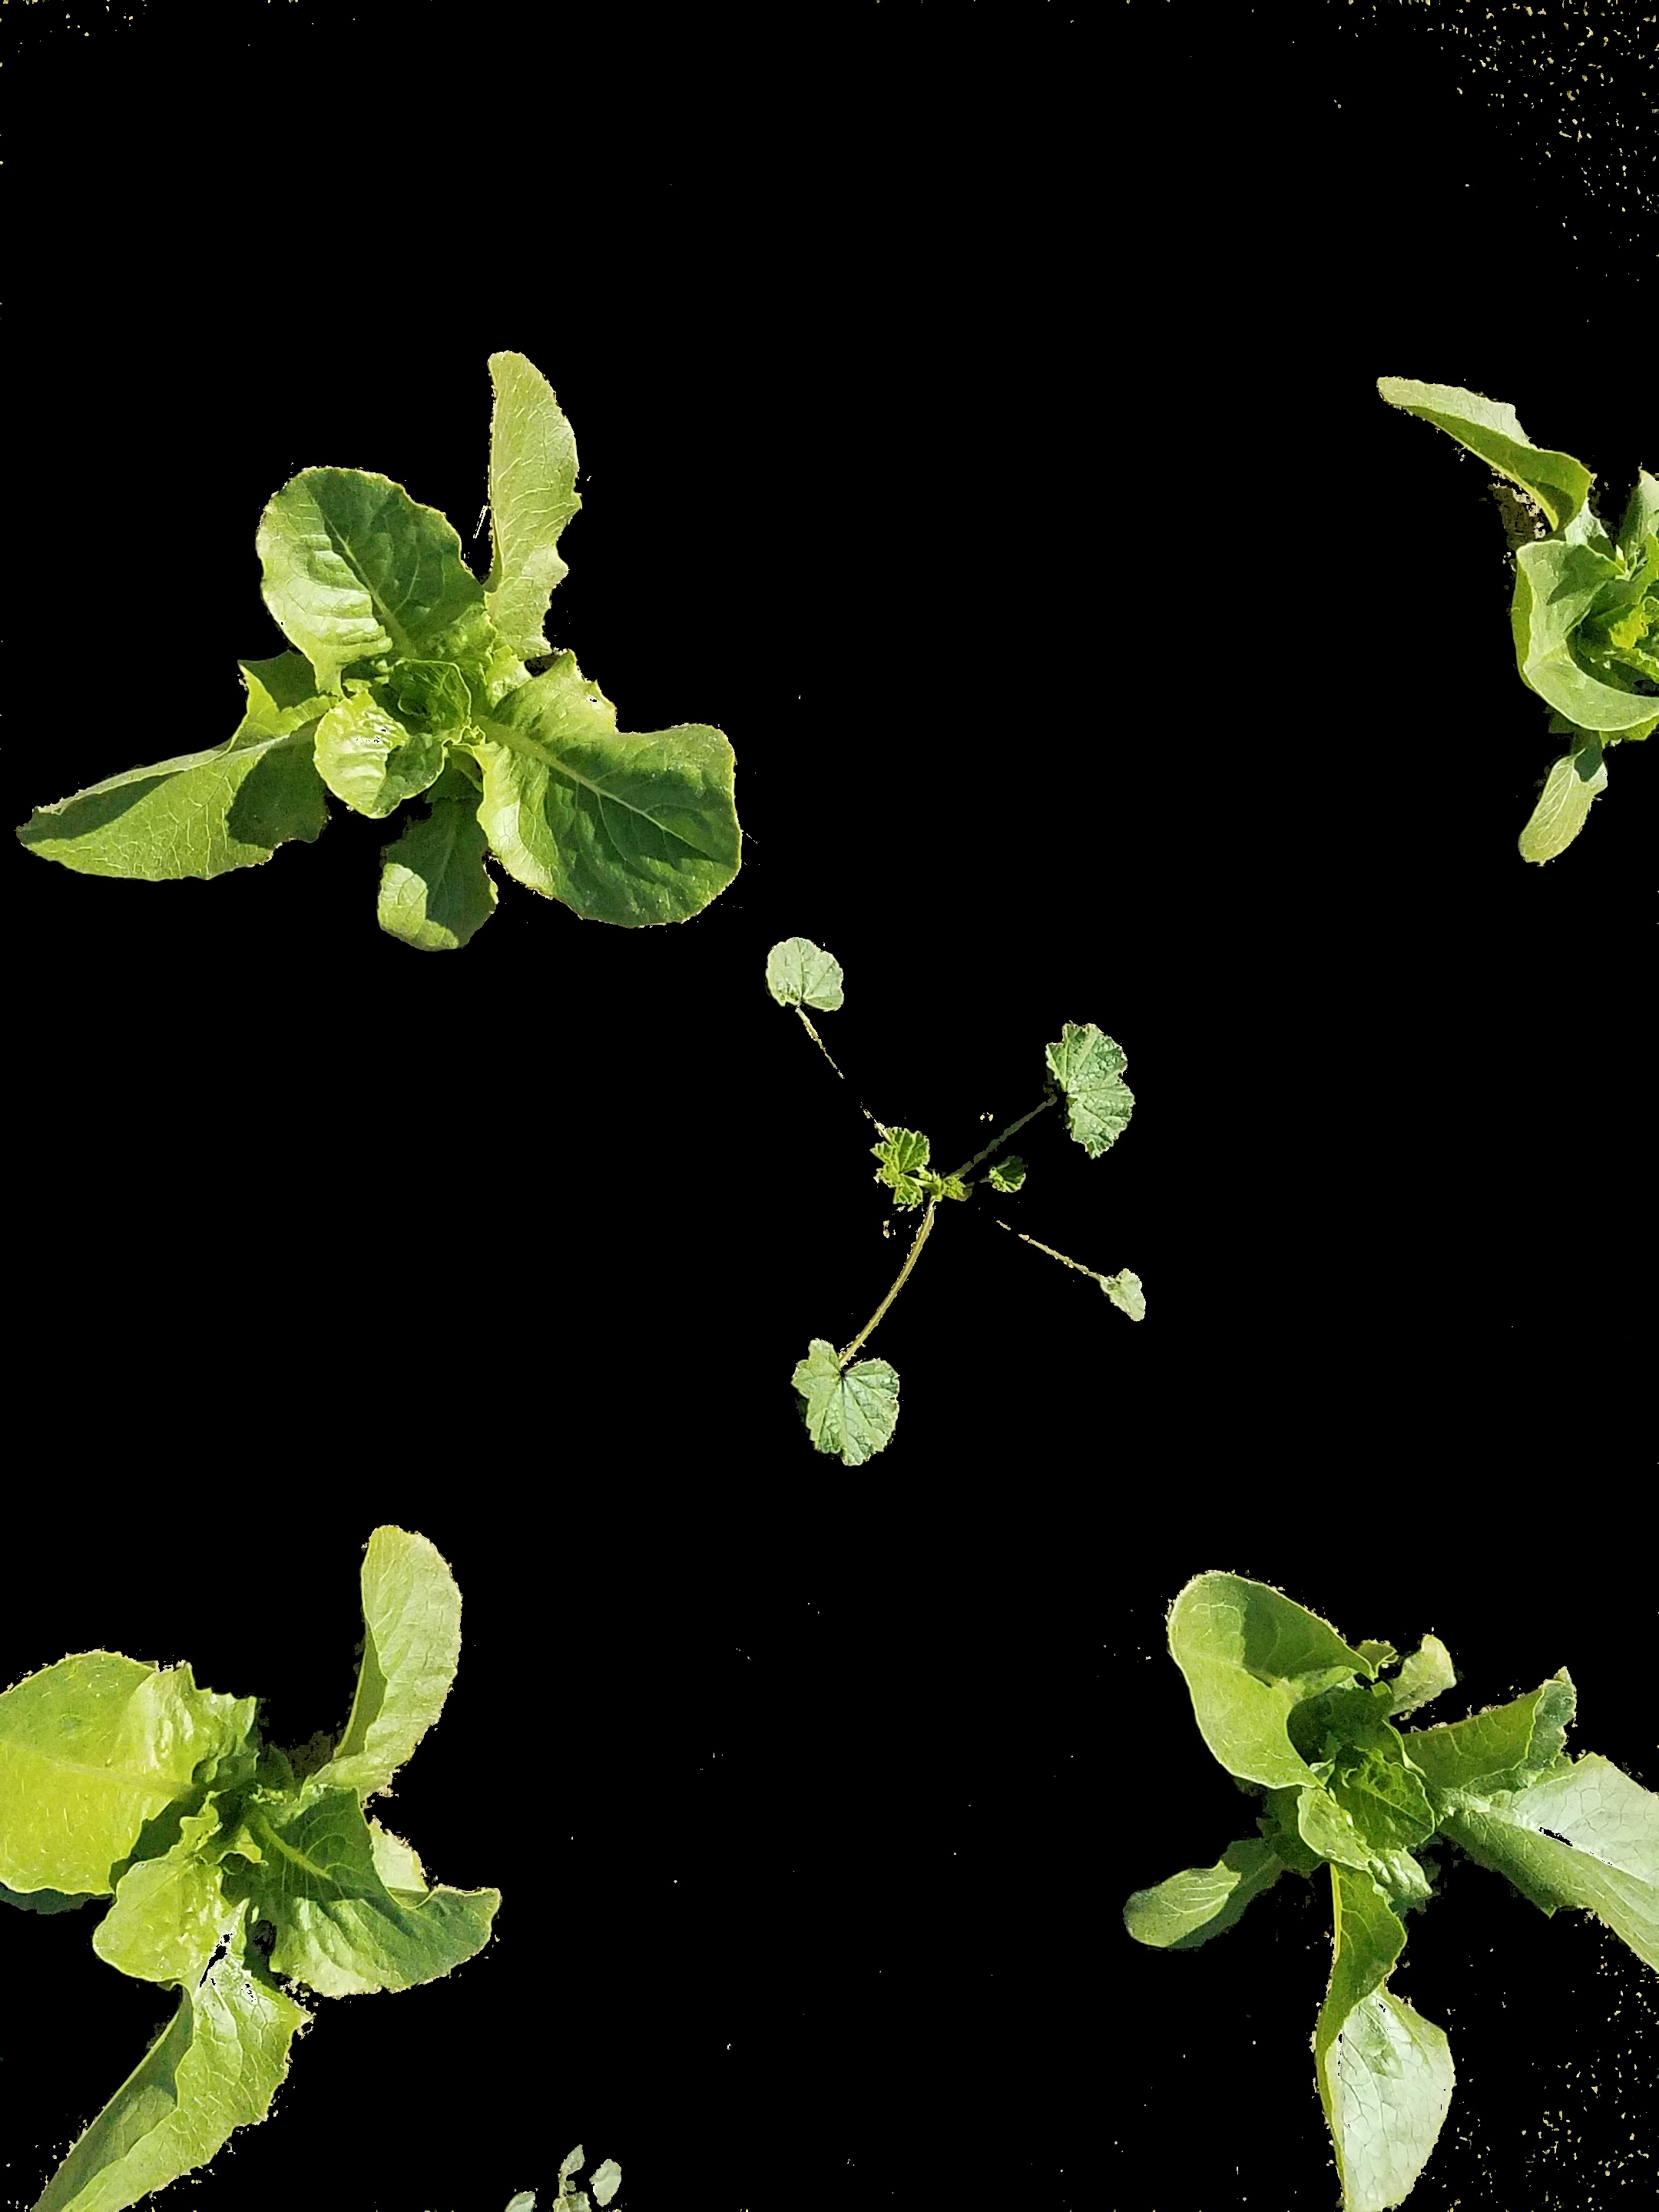
\includegraphics[width = 1.25in]{figures/20201117_112624-YI.jpg} \label{fig:yiq}} &
	\subfloat[Original]{\includegraphics[scale=0.0415,angle=90]{figures/20201117_112624.jpg} \label{fig:original}} \\
	\end{tabular}
	\caption[Segmentation results from various colorspaces outside RGB]{Segmentation results from various colorspaces outside RGB. The \ref{fig:ci} and \ref{fig:yiq} segmentation approaches are relatively clean, providing vegetation images that are free of ground clutter. The other three approaches, while providing good vegetation images, show too much of the ground, particularly in areas near to a plant, likely due to color contamination in the shadow area}
	\label{figure:results-colorspaces}
\end{figure}


% Bar chart produced with this command
%  python evaluate-masks.py -i ../lib/mask.jpg -t ../lib/testing/20201117_112624
\begin{figure}[h]
	\centering
	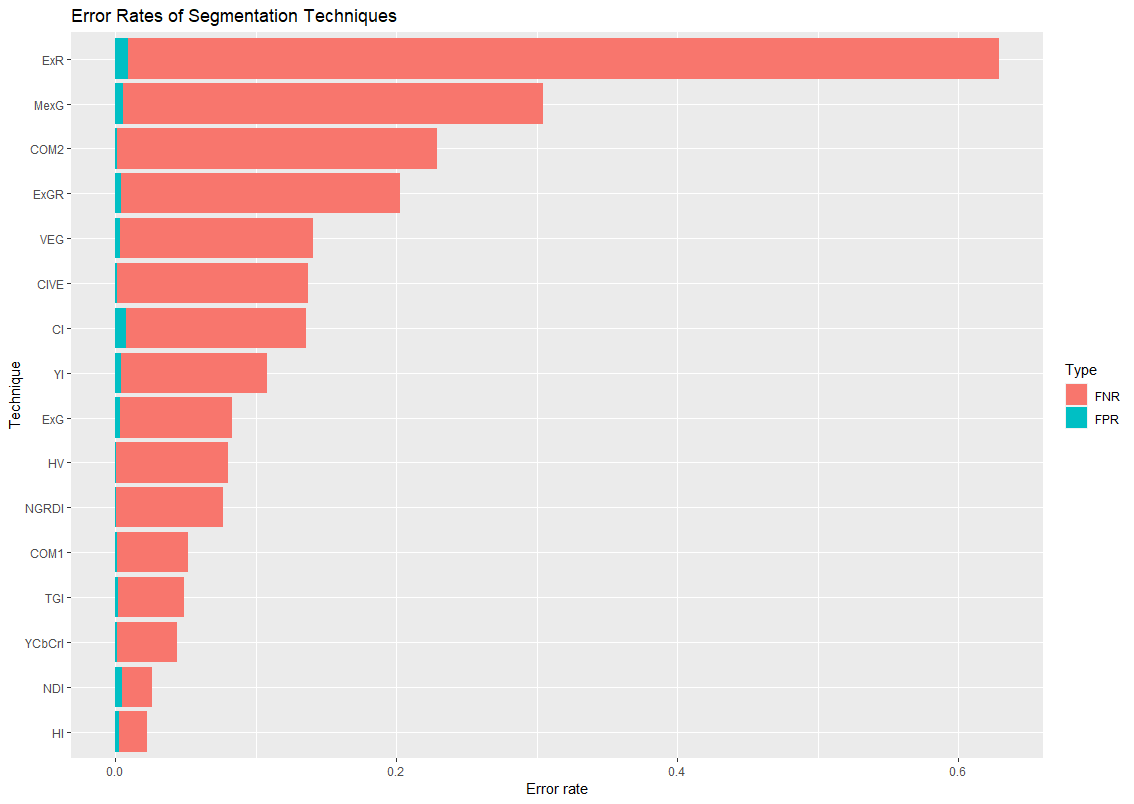
\includegraphics[width=.75\linewidth]{figures/segmentation-error-rates.png}
	\caption[Error rates of segmentation algorithms]{Average error rates for the images. Type I (Vegetation identified as ground) and Type II (Ground identified as vegetation) error are summarized by this figure. Of special note here are the errors encountered with NRGDI and HI approaches, as they represent clear differences in errors. The majority of the errors shown by the HI index mistakenly shows the ground as vegetation, with NDGRI  doing the opposite, hiding vegetation.}
	\label{fig:segmentation-errors}
\end{figure}

\subsubsection{Results}
Figures \ref{figure:results} and \ref{figure:results-colorspaces} demonstrate the effect of applying an index to an image, but visualizing the errors these indices make may prove insightful. While the errors encountered are shown more quantitatively in the chart of Figure \ref{fig:segmentation-errors}, a few qualitative observations are worthy of attention.  Figure~\ref{fig:overlay} shows a mask visualization overlayed on an image. In this instance, the mask is tinted red, so red covering vegetation is desired, and green vegetation is undesired. By combining the image with the mask it becomes a bit more clear where errors occur. Among other sources of error, two stand out: challenges in ambient lighting, and challenges of the subject itself.


\subsubsection{Problem: Reflections and Shadows}
Reflections within vegetation provide a challenge not easily surmounted.  In some cases, the area in reflection is not merely brighter than the surrounding pixels, but is completely devoid of usable pixels, as it is completely white (sometimes referenced as \textit{clipped}). This leads to the situation where portions of the vegetation are not present in the final segmented image, as the pixels do not contain the values associated with vegetation.  Deep shadows suffer from a problem similar to reflections in that they may be seen as nearly pure black. While mild shadows or reflections do not present much of a challenge, as vegetation in these areas typically have pixel values that are closely associated with their class. Reflections and shadows can be partially mitigated by a technique that improves the overall contrast of the image: \textit{histogram equalization}. Histogram equalization, for lack of a more precise description, stretches out the contrast over a broad range. While histogram equalization cannot reconstruct pixels than have been registered as pure white or pure black, this approach yields images with a more uniform intensity distribution.


% This produces figures that have aligned captions -- the [t] bit does the trick
\begin{figure}[H]
	\centering
	\subfloat[Leaf with reflection]{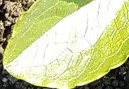
\includegraphics[width=.22\linewidth]{figures/reflection.jpg}\label{fig:leaf-with-reflection}}
	\hfill
	\subfloat[Before]{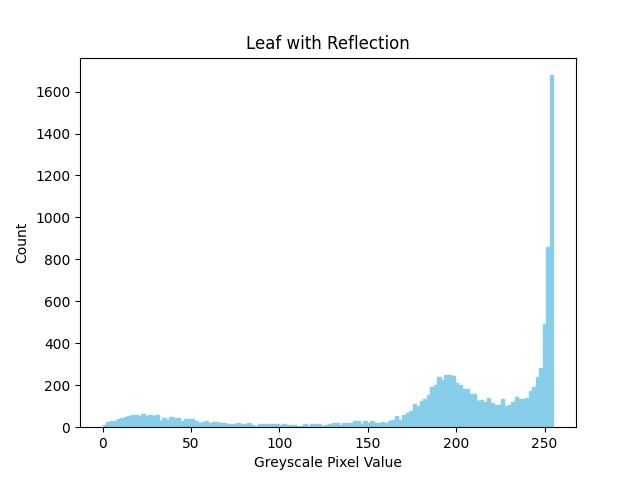
\includegraphics[width=.22\textwidth]{figures/reflection-histogram.jpg}\label{fig:reflection-histogram}}
	\hfill
	\subfloat[After equalization]{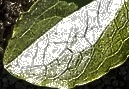
\includegraphics[width=.22\textwidth]{figures/reflection.equalized.jpg}\label{fig:leaf-equalized}}
	\hfill
	\subfloat[After equalization]{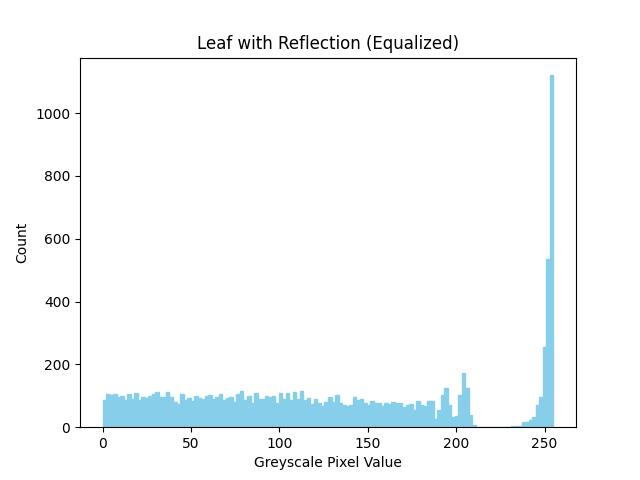
\includegraphics[width=.22\textwidth]{figures/reflection-histogram-equalized.jpg}\label{fig:leaf-equalized-histogram}}
	\caption[Reflection problems in segmented vegetation]{Reflections may be clipped (completely white) containing no usable information. While histogram equalization improves the image somewhat, applying that technique cannot reconstruct pixels that have been recorded as pure white. Figure \ref{fig:leaf-with-reflection} shows a portion of an image with a reflection strong enough to render a significant portion of the image unusable. Note the pixel count for pure or nearly pure white pixels in both \ref{fig:reflection-histogram} and \ref{fig:leaf-equalized-histogram} remain constant.  Those pixels should contain values indicative of vegetation. Aside from being a bit more pleasant to look at, these images differ in way that may have an impact on threshold selection. Note that the histogram of \ref{fig:reflection-histogram} no longer has the same shape, as intensities have be redistributed, eliminating the small bump.}
	\label{fig:reflection}
\end{figure}

\subsubsection{Color problems}
\label{section:problems-color}
Many of the indexes suffer from the same problem: they are focused on vegetation being green. Green stems and leaves are easily detected, but stems and leaves of other colors are not. Consider commonly encountered red-leaf lettuce. Depending on the stage of development and the angle of view, the leaves can be partially or entirely red (or a deep purple color). This is not limited to crops, of course, weeds such as redroot pigweed (\textit{Amaranthus retroflexus}) have red at the base of the leaves. Likewise, some weeds exhibit red stems. Purslane (\textit{Portulaca oleracea}) has red stems, and as an added complication, red edges on the leaves. Attempts to reveal the stems are complicated by the ground often containing a strong red coloration. Unfortunately, the band of color featured in the stems (red) is frequently found in the background (soil), so attempts to make the stems appear in the masked image are problematic, as this solution tends to bring unwanted ground pixels in the final image that contain hues found within the stems. The result of this is that the non-green portions of the vegetation does not appear in the resulting segmentation.  Even predominately green vegetation has non-green portions. Flowers are often missed by a green-centric index. While the omission of flowers may be desirable in further processing, if the flower obscures green vegetation that would otherwise be identified as such, that complicates further processing, especially when the green portion is significantly obscured. Uncorrected colors also complicate segmentation, as the same plant's leaves may be captured differently with two different cameras or under different lighting conditions. Under controlled lighting conditions (such as would be encountered in an enclosed system) color calibration is not essential every time, but systems that use ambient lighting require calibration each time to achieve optimal results. While the loss of red portions of the plant may not be a significant factor in subsequent processing, this should be taken into account. It may be the case that a single plant appears to be many more, as seen in \ref{fig:ndi}.
Even green portions of the vegetation may be green ``enough''. The segmented images in Figure \ref{figure:results} have discarded ground pixels while retaining most of the vegetated pixels that will be used is subsequent processing, but a close examination reveals that pixels in the stems of the weed in the center are also eliminated, as they are less green than the rest of the plant. Likewise, immature vegetation where stems are not sufficiently green will not appear in the final image.


\begin{figure}[H]
	\centering
	\subfloat[Field view of Purslane]{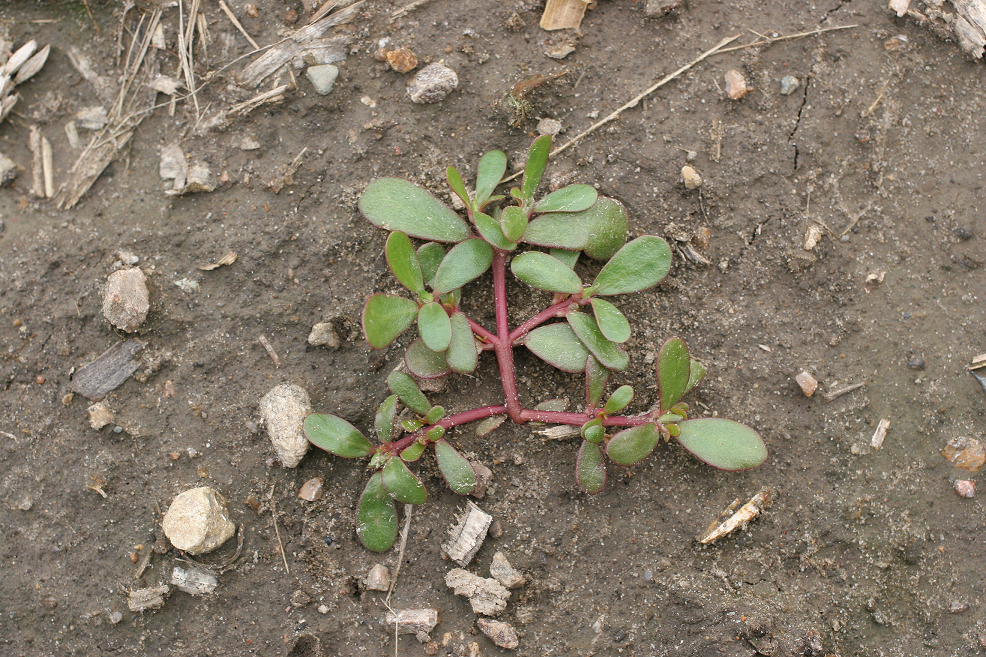
\includegraphics[width=.3\linewidth]{figures/purslane.png}\label{fig:purslane-original}}
	\hfill
	\subfloat[Image processed with NDI]{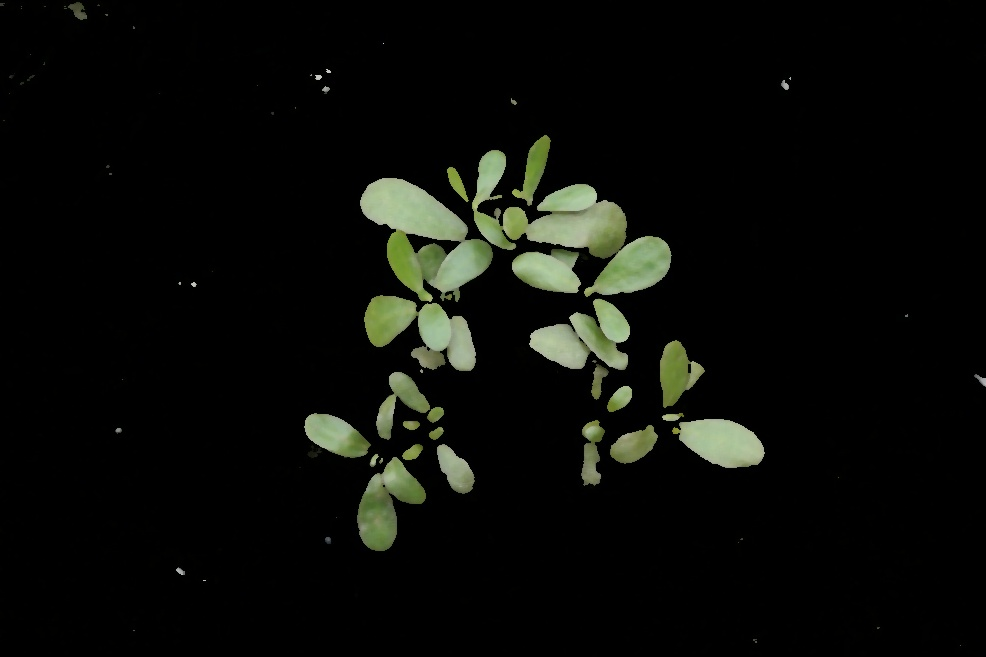
\includegraphics[width=.3\linewidth]{figures/ndi-purslane.jpg}\label{fig:purslane-ndi}}
	\hfill
	% Bar chart produced with this command
	% python evaluate-masks.py -i c:\uofa\weeds\lib\testing\IMG_1133 -s c:\uofa\maricopa\corrected\2024-04-24\iphone-drip\IMG_1133.jpg -t d:\maricopa\masks\2024-04-24\IMG_1133-mask.jpg -l ..\jetson\logging.ini
	\subfloat[Error rates]{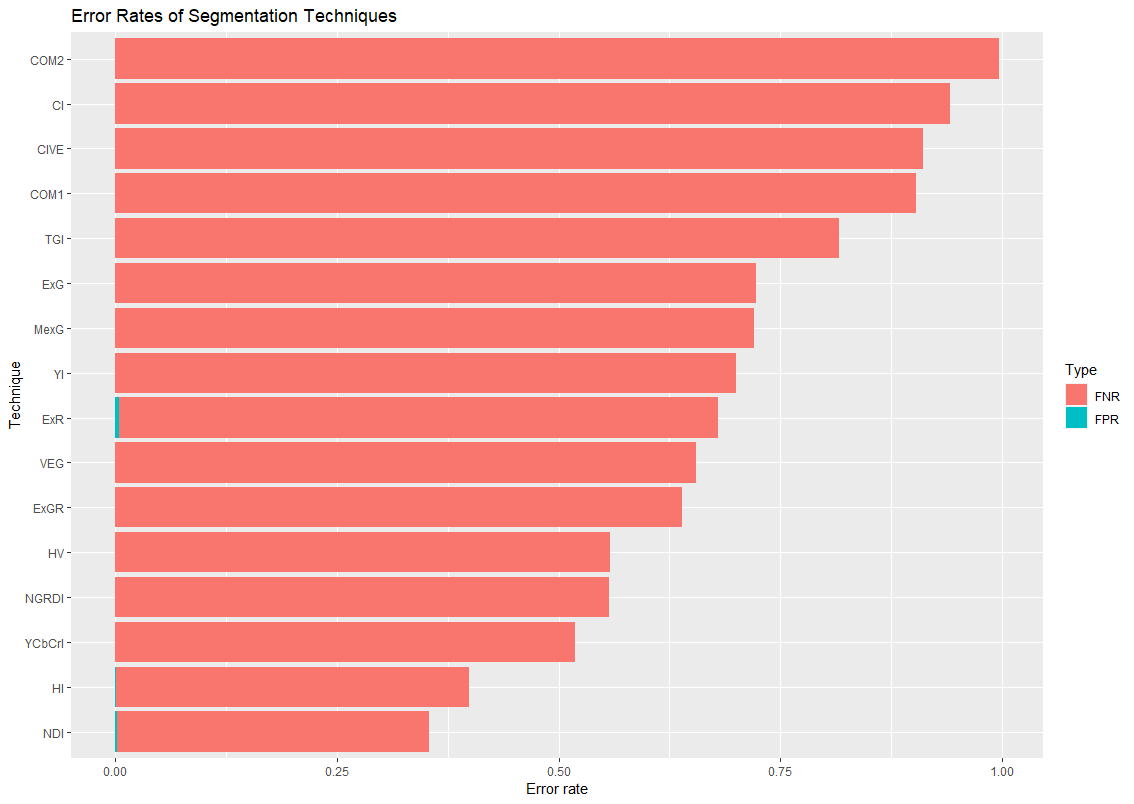
\includegraphics[width=.3\linewidth]{figures/segmentation-error-rates-color.png}\label{fig:error-rates}}
	\caption[Missing red portions of vegetation]{The red portions of the vegetation are missing after the index has been applied, as \ref{fig:purslane-ndi} shows. While the absence of stems may not affect further image processing using factors like leaf texture in classification, the absence of the red portions of features such as leaves may complicate attempts to use factors that are affected such as shape. As \ref{fig:error-rates} shows, the presence of red in a significant portion of the vegetation has a negative impact on the error rates of the algorithms examined}
	\label{fig:segmentation-color-problem}
\end{figure}

\subsection{Classification Based}
\label{section:classification}
A different approach is to classify each of the pixels in an image as belonging to one of two classes: vegetation or ground (This is often referred to as \textit{semantic segmentation}) Table \ref{table:ml-segmentation} shows the results of building models using the following approaches:  Support Vector Machine, Linear Discriminant Analysis, and Multi-layer Perceptron (MLP)\endnote{These implementations were provided in this \textit{scikit-learn} Python package.}. Each technique was applied to these color spaces: RGB, YIQ, YUV, HSI, HSV, YCbCr, and CIELab. A set of images taken from 2M AGL was selected and 20 samples taken from each of the 58 images, 10 ground points and 10 vegetation points. The term \textit{samples} in this context means that for each of the points sampled, the values for each of the color spaces identified in Section \ref{section:classification} were recorded. Based on these sample points, models were created and trained on 60\% of the data using the Scikit-learn Python library. While the RGB color space is commonly encountered, using it did not produce the best results for any of the techniques examined. That distinction tended to be -- but not always was -- the YIQ space. There are some important exceptions to keep in mind, particularly the performance of LDA, where identical scores for both RGB and YIQ spaces are seen. Using these classification approaches is not particularly pragmatic from a realtime perspective, as classifying every pixel in a modest 12MP image can take several hours on a modestly powerful CPU.
%\footnote{An approach optimized for a GPU would, no doubt, be much faster, but that is an exercise that is beyond the scope of this document}

%
% Begin Copied Table from this command
% python segment.py -i images -o segmented -t ../util/segmentation-training.csv  -b -s -l logging.ini -a all
% Minor manual edit: Remove leading space from header lines

Table \ref{table:ml-segmentation} shows a summary of the three classification approaches in various color spaces, giving the Area Under the Curve (AUC), Precision, Recall, and F1 scores. And while the the scores reported are encouraging, the resulting segmented images are not.

% Spacing between the rows
\renewcommand*{\arraystretch}{1.1}

%
% Begin Copied Table from this command
% python segment.py -i images -o segmented -t ../util/segmentation-training.csv  -b -s -l logging.ini -a all
% Minor manual edit: Remove leading space from header lines & data


\begin{longtable}{llrrrr}
\caption[Machine Learning Segmentation]{Machine Learning Segmentation}
\label{table:ml-segmentation}\\
\toprule
Technique &  Color &  AUC & Precision & Recall &   F1 \\
\midrule
\endfirsthead
\caption[]{Machine Learning Segmentation} \\
\toprule
Technique &  Color &  AUC & Precision & Recall &   F1 \\
\midrule
\endhead
\midrule
\multicolumn{6}{r}{{Continued on next page}} \\
\midrule
\endfoot

\bottomrule
\endlastfoot
MLP &RGB & 0.93 &      0.88 &   0.95 & 0.91 \\
MLP &YIQ & 0.94 &      0.88 &   0.96 & 0.92 \\
MLP &YUV & 0.94 &      0.88 &   0.96 & 0.92 \\
MLP &HSI & 0.91 &      0.86 &   0.94 & 0.90 \\
MLP &HSV & 0.90 &      0.87 &   0.94 & 0.91 \\
MLP &YCBCR & 0.94 &      0.88 &   0.96 & 0.92 \\
MLP &CIELAB & 0.94 &      0.88 &   0.96 & 0.92 \\
LDA &RGB & 0.94 &      0.88 &   0.96 & 0.92 \\
LDA &YIQ & 0.94 &      0.88 &   0.96 & 0.92 \\
LDA &YUV & 0.94 &      0.88 &   0.96 & 0.92 \\
LDA &HSI & 0.91 &      0.86 &   0.95 & 0.90 \\
LDA &HSV & 0.90 &      0.86 &   0.95 & 0.90 \\
LDA &YCBCR & 0.94 &      0.88 &   0.96 & 0.92 \\
LDA &CIELAB & 0.94 &      0.88 &   0.96 & 0.92 \\
SVM &RGB & 0.94 &      0.89 &   0.96 & 0.92 \\
SVM &YIQ & 0.92 &      0.88 &   0.82 & 0.85 \\
SVM &YUV & 0.93 &      0.86 &   0.93 & 0.89 \\
SVM &HSI & 0.91 &      0.87 &   0.94 & 0.90 \\
SVM &HSV & 0.90 &      0.87 &   0.94 & 0.90 \\
SVM &YCBCR & 0.92 &      0.85 &   0.91 & 0.88 \\
SVM &CIELAB & 0.91 &      0.86 &   0.96 & 0.90 \\
\end{longtable}

% 
% End copied table
%

\subsection{Semantic Segmentation}
Semantic segmentation is a convolutional neural network (CNN) using a trained model to classify each pixel in an image with a class label.  For the most part, agricultural images contain only two things: plants and the ground. While there are exceptions to this, of course, as images may include debris on the ground, irrigation equipment, etc., but from another viewpoint, images contain pixels that are plants and pixels that aren't.  The focus here is not to actually classify what each pixel represents (a brocolli plant, a segment of pipe, the ground, etc.), but to produce a mask that can be applied to the image to isolate vegetated pixels. This approach differs from the prior two approaches in that while index-based approaches consider no information about other images, and learning base approaches consider samples of a set of images to predict class membership, the deep-learning techniques considered in this section are trained on both images and the corresponding masks.

\subsubsection{U-Net}
The name of the U-Net architecture derives from the U-shaped arrangement of the downard decoder section and the upward encoder section. Developed initially for the segmentation of bio-medical images \cite{Ronneberger2015-ye}, this technique has been more widely adopted into various use cases.

\begin{figure}[H]
	\centering
	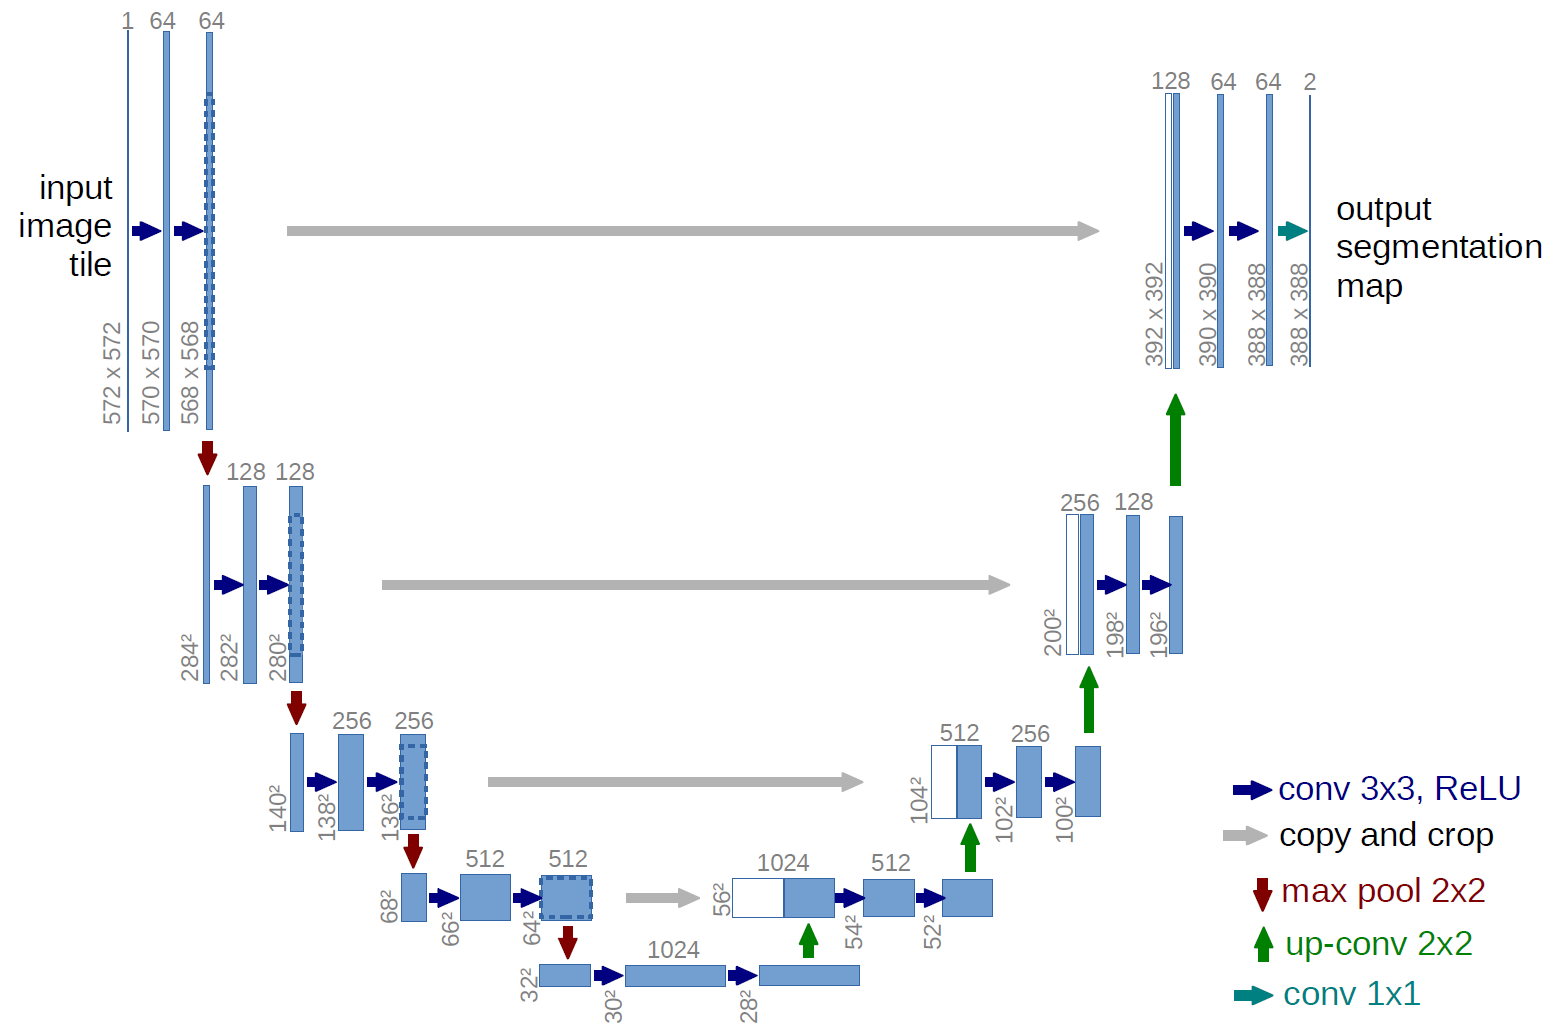
\includegraphics[height=5cm]{figures/u-net-architecture.png}
	\label{fig:u-net}
	\caption[U-Net architecture]{The name of U-Net architecture refers to the arrancement of decoders (often referred to as a contracting path) and encoders (the expanding path)}
\end{figure}
This architecture has a bit of a limitation that must be taken into acount in image sets: the length of each image's axis must be a mutiple of 32. That is, a 32x32 image will work, but a 32x90 image will not. The images and masked used for training and testing should be resized to fit this limitation. Using a model trained on images and associated masks from the MAC to a set of test images yields fairly low error rate masks when  those masks are evaluated against the ground truth: FPR of 0.0005 and FNR of 0.06, comparable to the lower rates achieved with some index-based approaches.

\begin{figure}[H]
	\centering
	\subfloat[Ground truth mask]{
\includegraphics[width=.3\linewidth]{figures/IMG_1115-mask.jpg}}
	\label{fig:original}
	\hfill
	\subfloat[U-Net mask]{
\includegraphics[width=.3\linewidth]{figures/IMG_1115-mask-unet.png}}
	\label{fig:mask}
	\hfill
	\subfloat[Apply U-Net mask]{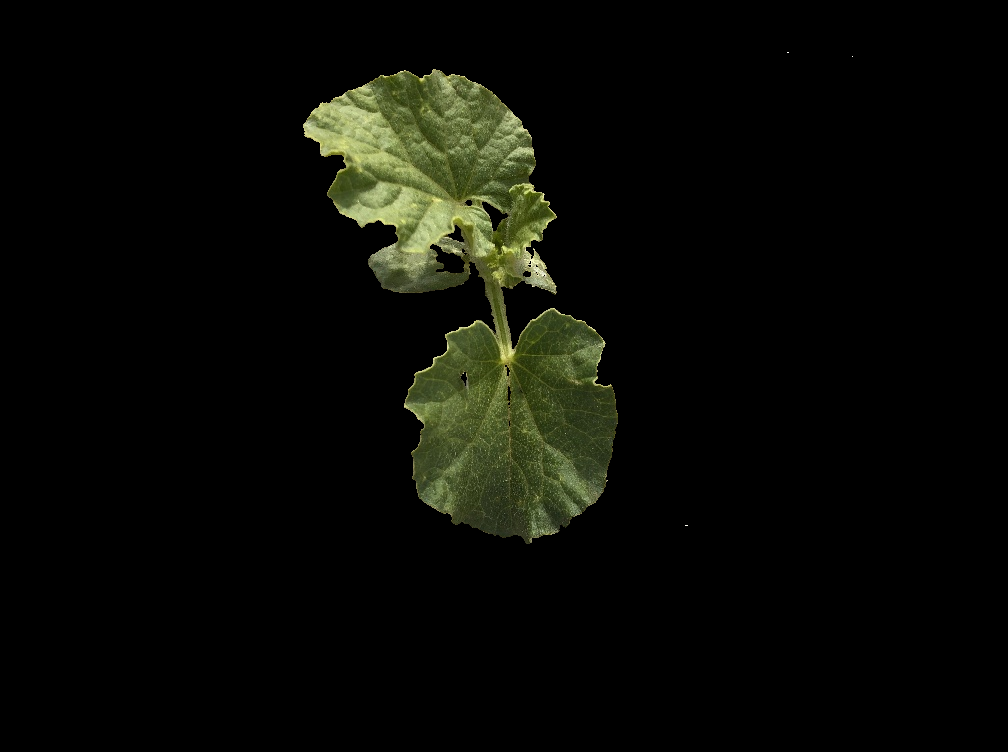
\includegraphics[width=.3\linewidth]{figures/IMG_1115-original-masked.png}}
	\label{fig:original-masked}
	\caption[U-Net segmentation vs ground truth]{The mask produced with U-Net shows some errors within the leaf, but is quite close to a match for the ground truth.}
	\label{fig:u-net-segmentation}
\end{figure}

\section{Discussion}
Image segmentation is typically a prelude to subsequent processing, not typically a standalone activity. Processing time of an image limits the forward speed of a system consuming those images in the field, but may not be a concern for systems that process images in a data-center application where timing is not a primary concern. That is, a segmentation approach that consumes 500 ms to process 500 cm of ground has limited forward progress to 3.6 kph (subsequent processing, such as classification and treatment plans would limit the speed further, of course, so this is just a floor on what the eventual speed would be). A salient advantage of index-based techniques is that they are computationally inexpensive. While this document did not provide or analyze timing results, it is realistic to compute an index for an image on a system without the assistance of a GPU within a 80 milliseconds or so. An important caveat should be kept in mind here, however. All software was written in an interpreted language, Python. While the index computation routines themselves cannot be meaningfully optimized, migrating the same routines to a compiled language (C, C++) yields much lower numbers. An index calculation can realistically be performed in a few milliseconds in that environment. 
Machine learning approaches using techniques (Support Vector Machine, KNN, Logistic Regression, etc.) to classify every pixel yield good results, but, from a compute-time perspective, it is not feasible to incorporate that approach into a system with real-time demands. While classification time varies, multiple seconds are typically required to segment a single image. Deep Learning with U-Net, while not as time consuming as the figures quoted for Machine Learning, are fairly fast, but not particularly suitable for a real-time system processing images fast enough to allow commercially viable speeds. Image mask production required 200 milliseconds with the assist of a GPU, 400 milliseconds using only the CPU. \endnote{All processing was performed on a system with an 11th Gen Intel(R) Core(TM) i7-11700F @ 2.50GHz   2.50 GHz CPU and an NVIDIA GeoForce GTX 1660 SUPER GPU, using Python 3.6.9. While this combination is modest, comparable systems can be used for deployment in field systems.}

While it may be tempting to choose the most accurate approach for a segmentation system, any selection must answer an important question: \textit{does the mechanism matter that much?} If the accuracy of segmentation negatively impacts the accuracy of subsequent processing (likely classification), then the answer is that it does matter. Further investigation is required to answer this question. Whereas an index-based approach such as Excessive Red did not perform as well as Com1 demonstrated, if the classification method focused on characteristics of the interior of the leaf (texture, for example) segmentation error that resulted in distortions in other factors (shape, for instance), may not negatively impact classification accuracy.


% Original MDPI Template Follows
%\subsection{Subsection}
%\subsubsection{Subsubsection}
%
%Bulleted lists look like this:
%\begin{itemize}
%\item	First bullet;
%\item	Second bullet;
%\item	Third bullet.
%\end{itemize}
%
%Numbered lists can be added as follows:
%\begin{enumerate}
%\item	First item; 
%\item	Second item;
%\item	Third item.
%\end{enumerate}
%
%The text continues here.
%
%\subsection{Figures, Tables and Schemes}
%
%All figures and tables should be cited in the main text as Figure~\ref{fig1}, Table~\ref{tab1}, etc.
%
%\begin{figure}[H]
%%\isPreprints{\centering}{} % Only used for preprints
%
\includegraphics[width=7 cm]{Definitions/logo-mdpi}
%\caption{This is a figure. Schemes follow the same formatting.\label{fig1}}
%\end{figure}   
%\unskip
%
%\begin{table}[H] 
%%\tablesize{\small}
%\caption{This is a table caption. Tables should be placed in the main text near to the first time they are~cited.\label{tab1}}
%%\isPreprints{\centering}{} % Only used for preprints
%\begin{tabularx}{\textwidth}{CCC}
%\toprule
%\textbf{Title 1}	& \textbf{Title 2}	& \textbf{Title 3}\\
%\midrule
%Entry 1		& Data			& Data\\
%Entry 2		& Data			& Data \textsuperscript{1}\\
%\bottomrule
%\end{tabularx}
%
%\noindent{\footnotesize{\textsuperscript{1} Tables may have a footer.}}
%\end{table}
%
%The text continues here (Figure~\ref{fig2} and Table~\ref{tab2}).
%
%% Example of a figure that spans the whole page width and with subfigures. The same concept works for tables, too.
%\begin{figure}[H]
%\centering
%%\isPreprints{}{% This command is only used for ``preprints''.
%\begin{adjustwidth}{-\extralength}{0cm}
%%} % If the paper is ``preprints'', please uncomment this parenthesis.
%\subfloat[\centering]{
\includegraphics[width=7.7cm]{Definitions/logo-mdpi}}
%\hfill
%\subfloat[\centering]{
\includegraphics[width=7.7cm]{Definitions/logo-mdpi}}\\
%\subfloat[\centering]{
\includegraphics[width=7.7cm]{Definitions/logo-mdpi}}
%\hfill
%\subfloat[\centering]{
\includegraphics[width=7.7cm]{Definitions/logo-mdpi}}
%%\isPreprints{}{% This command is only used for ``preprints''.
%\end{adjustwidth}
%%} % If the paper is ``preprints'', please uncomment this parenthesis.
%\caption{This is a wide figure. Schemes follow the same formatting. If there are multiple panels, they should be listed as: (\textbf{a}) Description of what is contained in the first panel. (\textbf{b}) Description of what is contained in the second panel. (\textbf{c}) Description of what is contained in the third panel. (\textbf{d}) Description of what is contained in the fourth panel. Figures should be placed in the main text near to the first time they are cited. A caption on a single line should be centered.\label{fig2}}
%\end{figure} 
%
%\begin{table}[H]
%\caption{This is a wide table.\label{tab2}}
%%\isPreprints{\centering}{% This command is only used for ``preprints''.
%	\begin{adjustwidth}{-\extralength}{0cm}
%%} % If the paper is ``preprints'', please uncomment this parenthesis.
%%\isPreprints{\begin{tabularx}{\textwidth}{CCCC}}{% This command is only used for ``preprints''.
%		\begin{tabularx}{\fulllength}{CCCC}
%%} % If the paper is ``preprints'', please uncomment this parenthesis.
%			\toprule
%			\textbf{Title 1}	& \textbf{Title 2}	& \textbf{Title 3}     & \textbf{Title 4}\\
%			\midrule
%\multirow[m]{3}{*}{Entry 1 *}	& Data			& Data			& Data\\
%			  	                   & Data			& Data			& Data\\
%			             	      & Data			& Data			& Data\\
%                   \midrule
%\multirow[m]{3}{*}{Entry 2}    & Data			& Data			& Data\\
%			  	                  & Data			& Data			& Data\\
%			             	     & Data			& Data			& Data\\
%			\bottomrule
%		\end{tabularx}
%%		\isPreprints{}{% This command is only used for ``preprints''.
%	\end{adjustwidth}
%%} % If the paper is ``preprints'', please uncomment this parenthesis.
%	\noindent{\footnotesize{* Tables may have a footer.}}
%\end{table}
%
%%\begin{listing}[H]
%%\caption{Title of the listing}
%%\rule{\columnwidth}{1pt}
%%\raggedright Text of the listing. In font size footnotesize, small, or normalsize. Preferred format: left aligned and single spaced. Preferred border format: top border line and bottom border line.
%%\rule{\columnwidth}{1pt}
%%\end{listing}
%
%Text.
%
%Text.
%
%\subsection{Formatting of Mathematical Components}
%
%This is the example 1 of equation:
%\begin{linenomath}
%\begin{equation}
%a = 1,
%\end{equation}
%\end{linenomath}
%the text following an equation need not be a new paragraph. Please punctuate equations as regular text.
%%% If the documentclass option "submit" is chosen, please insert a blank line before and after any math environment (equation and eqnarray environments). This ensures correct linenumbering. The blank line should be removed when the documentclass option is changed to "accept" because the text following an equation should not be a new paragraph.
%
%This is the example 2 of equation:
%%\isPreprints{}{% This command is only used for ``preprints''.
%\begin{adjustwidth}{-\extralength}{0cm}
%%} % If the paper is ``preprints'', please uncomment this parenthesis.
%\begin{equation}
%a = b + c + d + e + f + g + h + i + j + k + l + m + n + o + p + q + r + s + t + u + v + w + x + y + z
%\end{equation}
%%\isPreprints{}{% This command is only used for ``preprints''.
%\end{adjustwidth}
%%} % If the paper is ``preprints'', please uncomment this parenthesis.
%
%%% Example of a page in landscape format (with table and table footnote).
%%\startlandscape
%%\begin{table}[H] %% Table in wide page
%%%\isPreprints{\centering}{} % This command is only used for ``preprints''.
%%\caption{This is a very wide table.\label{tab3}}
%%	\begin{tabularx}{\textwidth}{CCCC}
%%		\toprule
%%		\textbf{Title 1}	& \textbf{Title 2}	& \textbf{Title 3}	& \textbf{Title 4}\\
%%		\midrule
%%		Entry 1		& Data			& Data			& This cell has some longer content that runs over two lines.\\
%%		Entry 2		& Data			& Data			& Data\textsuperscript{1}\\
%%		\bottomrule
%%	\end{tabularx}
%%%\isPreprints{}{% This command is only used for ``preprints''.
%%	\begin{adjustwidth}{+\extralength}{0cm}
%%%} % If the paper is ``preprints'', please uncomment this parenthesis.
%%		\noindent\footnotesize{\textsuperscript{1} This is a table footnote.}
%%%\isPreprints{}{% This command is only used for ``preprints''.
%%	\end{adjustwidth}
%%%} % If the paper is ``preprints'', please uncomment this parenthesis.
%%\end{table}
%%\finishlandscape
%
%
%Please punctuate equations as regular text. Theorem-type environments (including propositions, lemmas, corollaries etc.) can be formatted as follows:
%%% Example of a theorem:
%\begin{Theorem}
%Example text of a theorem.
%\end{Theorem}
%
%The text continues here. Proofs must be formatted as follows:
%
%%% Example of a proof:
%\begin{proof}[Proof of Theorem 1]
%Text of the proof. Note that the phrase ``of Theorem 1'' is optional if it is clear which theorem is being referred to.
%\end{proof}
%The text continues here.
%
%%%%%%%%%%%%%%%%%%%%%%%%%%%%%%%%%%%%%%%%%%%
%\section{Discussion}
%
%Authors should discuss the results and how they can be interpreted from the perspective of previous studies and of the working hypotheses. The findings and their implications should be discussed in the broadest context possible. Future research directions may also be highlighted.
%
%%%%%%%%%%%%%%%%%%%%%%%%%%%%%%%%%%%%%%%%%%%
%\section{Conclusions}
%
%This section is not mandatory, but can be added to the manuscript if the discussion is unusually long or complex.
%
%%%%%%%%%%%%%%%%%%%%%%%%%%%%%%%%%%%%%%%%%%%
%\section{Patents}
%
%This section is not mandatory, but may be added if there are patents resulting from the work reported in this manuscript.
%
%%%%%%%%%%%%%%%%%%%%%%%%%%%%%%%%%%%%%%%%%%%
%\vspace{6pt} 
%
%%%%%%%%%%%%%%%%%%%%%%%%%%%%%%%%%%%%%%%%%%%
%%% optional
%%\supplementary{The following supporting information can be downloaded at:  \linksupplementary{s1}, Figure S1: title; Table S1: title; Video S1: title.}
%
%% Only for journal Methods and Protocols:
%% If you wish to submit a video article, please do so with any other supplementary material.
%% \supplementary{The following supporting information can be downloaded at: \linksupplementary{s1}, Figure S1: title; Table S1: title; Video S1: title. A supporting video article is available at doi: link.}
%
%% Only used for preprtints:
%% \supplementary{The following supporting information can be downloaded at the website of this paper posted on \href{https://www.preprints.org/}{Preprints.org}.}
%
%% Only for journal Hardware:
%% If you wish to submit a video article, please do so with any other supplementary material.
%% \supplementary{The following supporting information can be downloaded at: \linksupplementary{s1}, Figure S1: title; Table S1: title; Video S1: title.\vspace{6pt}\\
%%\begin{tabularx}{\textwidth}{lll}
%%\toprule
%%\textbf{Name} & \textbf{Type} & \textbf{Description} \\
%%\midrule
%%S1 & Python script (.py) & Script of python source code used in XX \\
%%S2 & Text (.txt) & Script of modelling code used to make Figure X \\
%%S3 & Text (.txt) & Raw data from experiment X \\
%%S4 & Video (.mp4) & Video demonstrating the hardware in use \\
%%... & ... & ... \\
%%\bottomrule
%%\end{tabularx}
%%}
%
%%%%%%%%%%%%%%%%%%%%%%%%%%%%%%%%%%%%%%%%%%%
% BEM -- not applicable
%\authorcontributions{For research articles with several authors, a short paragraph specifying their individual contributions must be provided. The following statements should be used ``Conceptualization, X.X. and Y.Y.; methodology, X.X.; software, X.X.; validation, X.X., Y.Y. and Z.Z.; formal analysis, X.X.; investigation, X.X.; resources, X.X.; data curation, X.X.; writing---original draft preparation, X.X.; writing---review and editing, X.X.; visualization, X.X.; supervision, X.X.; project administration, X.X.; funding acquisition, Y.Y. All authors have read and agreed to the published version of the manuscript.'', please turn to the  \href{http://img.mdpi.org/data/contributor-role-instruction.pdf}{CRediT taxonomy} for the term explanation. Authorship must be limited to those who have contributed substantially to the work~reported.}

\funding{This research received no external funding.}

%\institutionalreview{In this section, you should add the Institutional Review Board Statement and approval number, if relevant to your study. You might choose to exclude this statement if the study did not require ethical approval. Please note that the Editorial Office might ask you for further information. Please add “The study was conducted in accordance with the Declaration of Helsinki, and approved by the Institutional Review Board (or Ethics Committee) of NAME OF INSTITUTE (protocol code XXX and date of approval).” for studies involving humans. OR “The animal study protocol was approved by the Institutional Review Board (or Ethics Committee) of NAME OF INSTITUTE (protocol code XXX and date of approval).” for studies involving animals. OR “Ethical review and approval were waived for this study due to REASON (please provide a detailed justification).” OR “Not applicable” for studies not involving humans or animals.}

%\informedconsent{Any research article describing a study involving humans should contain this statement. Please add ``Informed consent was obtained from all subjects involved in the study.'' OR ``Patient consent was waived due to REASON (please provide a detailed justification).'' OR ``Not applicable'' for studies not involving humans. You might also choose to exclude this statement if the study did not involve humans.

%Written informed consent for publication must be obtained from participating patients who can be identified (including by the patients themselves). Please state ``Written informed consent has been obtained from the patient(s) to publish this paper'' if applicable.}

\dataavailability{All code used in the preparation of this paper is available from this github repository: https://github.com/evan-mcginnis/segmentation. Raw data is avaible upon request from the corresponding author.} 

% Only for journal Drones
%\durcstatement{Current research is limited to the [please insert a specific academic field, e.g., XXX], which is beneficial [share benefits and/or primary use] and does not pose a threat to public health or national security. Authors acknowledge the dual-use potential of the research involving xxx and confirm that all necessary precautions have been taken to prevent potential misuse. As an ethical responsibility, authors strictly adhere to relevant national and international laws about DURC. Authors advocate for responsible deployment, ethical considerations, regulatory compliance, and transparent reporting to mitigate misuse risks and foster beneficial outcomes.}

% Only for journal Nursing Reports
%\publicinvolvement{Please describe how the public (patients, consumers, carers) were involved in the research. Consider reporting against the GRIPP2 (Guidance for Reporting Involvement of Patients and the Public) checklist. If the public were not involved in any aspect of the research add: ``No public involvement in any aspect of this research''.}
%
%% Only for journal Nursing Reports
%\guidelinesstandards{Please add a statement indicating which reporting guideline was used when drafting the report. For example, ``This manuscript was drafted against the XXX (the full name of reporting guidelines and citation) for XXX (type of research) research''. A complete list of reporting guidelines can be accessed via the equator network: \url{https://www.equator-network.org/}.}
%
%% Only for journal Nursing Reports
%\useofartificialintelligence{Please describe in detail any and all uses of artificial intelligence (AI) or AI-assisted tools used in the preparation of the manuscript. This may include, but is not limited to, language translation, language editing and grammar, or generating text. Alternatively, please state that “AI or AI-assisted tools were not used in drafting any aspect of this manuscript”.}

\acknowledgments{Thanks to Drs. Diaa Elshika and Said Atallah of the University of Arizona for access to the fields where images were acquired.}

\conflictsofinterest{None.} 

%%%%%%%%%%%%%%%%%%%%%%%%%%%%%%%%%%%%%%%%%%
%% Optional

%% Only for journal Encyclopedia
%\entrylink{The Link to this entry published on the encyclopedia platform.}

%
% BEM -- all terms should be defined in text -- not needed
%\abbreviations{Abbreviations}{
%The following abbreviations are used in this manuscript:\\
%
%\noindent 
%\begin{tabular}{@{}ll}
%MDPI & Multidisciplinary Digital Publishing Institute\\
%DOAJ & Directory of open access journals\\
%TLA & Three letter acronym\\
%LD & Linear dichroism
%\end{tabular}
%}

%%%%%%%%%%%%%%%%%%%%%%%%%%%%%%%%%%%%%%%%%%
%% Optional
%% BEM -- not needed 
%%\appendixtitles{no} % Leave argument "no" if all appendix headings stay EMPTY (then no dot is printed after "Appendix A"). If the appendix sections contain a heading then change the argument to "yes".
%%\appendixstart
%%\appendix
%%\section[\appendixname~\thesection]{}
%%\subsection[\appendixname~\thesubsection]{}
%%The appendix is an optional section that can contain details and data supplemental to the main text---for example, explanations of experimental details that would disrupt the flow of the main text but nonetheless remain crucial to understanding and reproducing the research shown; figures of replicates for experiments of which representative data are shown in the main text can be added here if brief, or as Supplementary Data. Mathematical proofs of results not central to the paper can be added as an appendix.
%%
%%\begin{table}[H] 
%%\caption{This is a table caption.\label{tab5}}
%%%\newcolumntype{C}{>{\centering\arraybackslash}X}
%%\begin{tabularx}{\textwidth}{CCC}
%%\toprule
%%\textbf{Title 1}	& \textbf{Title 2}	& \textbf{Title 3}\\
%%\midrule
%%Entry 1		& Data			& Data\\
%%Entry 2		& Data			& Data\\
%%\bottomrule
%%\end{tabularx}
%%\end{table}
%%
%%\section[\appendixname~\thesection]{}
%%All appendix sections must be cited in the main text. In the appendices, Figures, Tables, etc. should be labeled, starting with ``A''---e.g., Figure A1, Figure A2, etc.

%%%%%%%%%%%%%%%%%%%%%%%%%%%%%%%%%%%%%%%%%%
%\isPreprints{} % If the paper is ``preprints'', please uncomment this parenthesis.
\printendnotes[custom] % Un-comment to print a list of endnotes

\reftitle{References}

% Please provide either the correct journal abbreviation (e.g. according to the “List of Title Word Abbreviations” http://www.issn.org/services/online-services/access-to-the-ltwa/) or the full name of the journal.
% Citations and References in Supplementary files are permitted provided that they also appear in the reference list here. 

%=====================================
% References, variant A: external bibliography
%=====================================
\bibliography{../paperpile.bib}

%=====================================
% References, variant B: internal bibliography
%=====================================

%% ACS format
%\isAPAandChicago{}{%
%\begin{thebibliography}{999}
%% Reference 1
%\bibitem[Author1(year)]{ref-journal}
%Author~1, T. The title of the cited article. {\em Journal Abbreviation} {\bf 2008}, {\em 10}, 142--149.
%% Reference 2
%\bibitem[Author2(year)]{ref-book1}
%Author~2, L. The title of the cited contribution. In {\em The Book Title}; Editor 1, F., Editor 2, A., Eds.; Publishing House: City, Country, 2007; pp. 32--58.
%% Reference 3
%\bibitem[Author1 and Author2 (year)]{ref-book2}
%Author 1, A.; Author 2, B. \textit{Book Title}, 3rd ed.; Publisher: Publisher Location, Country, 2008; pp. 154--196.
%% Reference 4
%\bibitem[Author4(year)]{ref-unpublish}
%Author 1, A.B.; Author 2, C. Title of Unpublished Work. \textit{Abbreviated Journal Name} year, \textit{phrase indicating stage of publication (submitted; accepted; in press)}.
%% Reference 5
%\bibitem[Author8(year)]{ref-url}
%Title of Site. Available online: URL (accessed on Day Month Year).
%% Reference 6
%\bibitem[Author6(year)]{ref-proceeding}
%Author 1, A.B.; Author 2, C.D.; Author 3, E.F. Title of presentation. In Proceedings of the Name of the Conference, Location of Conference, Country, Date of Conference (Day Month Year); Abstract Number (optional), Pagination (optional).
%% Reference 7
%\bibitem[Author7(year)]{ref-thesis}
%Author 1, A.B. Title of Thesis. Level of Thesis, Degree-Granting University, Location of University, Date of Completion.
%\end{thebibliography}
%}
%
%% Chicago format (Used for journal: arts, genealogy, histories, humanities, jintelligence, laws, literature, religions, risks, socsci)
%\isChicagoStyle{%
%\begin{thebibliography}{999}
%% Reference 1
%\bibitem[Aranceta-Bartrina(1999a)]{ref-journal}
%Aranceta-Bartrina, Javier. 1999a. Title of the cited article. \textit{Journal Title} 6: 100--10.
%% Reference 2
%\bibitem[Aranceta-Bartrina(1999b)]{ref-book1}
%Aranceta-Bartrina, Javier. 1999b. Title of the chapter. In \textit{Book Title}, 2nd ed. Edited by Editor 1 and Editor 2. Publication place: Publisher, vol. 3, pp. 54–96.
%% Reference 3
%\bibitem[Baranwal and Munteanu {[1921]}(1955)]{ref-book2}
%Baranwal, Ajay K., and Costea Munteanu. 1955. \textit{Book Title}. Publication place: Publisher, pp. 154--96. First published 1921 (op-tional).
%% Reference 4
%\bibitem[Berry and Smith(1999)]{ref-thesis}
%Berry, Evan, and Amy M. Smith. 1999. Title of Thesis. Level of Thesis, Degree-Granting University, City, Country. Identifi-cation information (if available).
%% Reference 5
%\bibitem[Cojocaru et al.(1999)]{ref-unpublish}
%Cojocaru, Ludmila, Dragos Constatin Sanda, and Eun Kyeong Yun. 1999. Title of Unpublished Work. \textit{Journal Title}, phrase indicating stage of publication.
%% Reference 6
%\bibitem[Driver et al.(2000)]{ref-proceeding}
%Driver, John P., Steffen Rohrs, and Sean Meighoo. 2000. Title of Presentation. In \textit{Title of the Collected Work} (if available). Paper presented at Name of the Conference, Location of Conference, Date of Conference.
%% Reference 7
%\bibitem[Harwood(2008)]{ref-url}
%Harwood, John. 2008. Title of the cited article. Available online: URL (accessed on Day Month Year).
%\end{thebibliography}
%}{}
%
%% APA format (Used for journal: admsci, behavsci, businesses, econometrics, economies, education, ejihpe, games, humans, ijfs, journalmedia, jrfm, languages, psycholint, publications, tourismhosp, youth)
%\isAPAStyle{%
%\begin{thebibliography}{999}
%% Reference 1
%\bibitem[\protect\citeauthoryear{Azikiwe \BBA\ Bello}{{2020a}}]{ref-journal}
%Azikiwe, H., \& Bello, A. (2020a). Title of the cited article. \textit{Journal Title}, \textit{Volume}(Issue), 
%Firstpage--Lastpage/Article Number.
%% Reference 2
%\bibitem[\protect\citeauthoryear{Azikiwe \BBA\ Bello}{{2020b}}]{ref-book1}
%Azikiwe, H., \& Bello, A. (2020b). \textit{Book title}. Publisher Name.
%% Reference 3
%\bibitem[Davison(1623/2019)]{ref-book2}
%Davison, T. E. (2019). Title of the book chapter. In A. A. Editor (Ed.), \textit{Title of the book: Subtitle} 
%(pp. Firstpage--Lastpage). Publisher Name. (Original work published 1623) (Optional).
%% Reference 4
%\bibitem[Fistek et al.(2017)]{ref-proceeding}
%Fistek, A., Jester, E., \& Sonnenberg, K. (2017, Month Day). Title of contribution [Type of contribution]. Conference Name, Conference City, Conference Country.
%% Reference 5
%\bibitem[Hutcheson(2012)]{ref-thesis}
%Hutcheson, V. H. (2012). \textit{Title of the thesis} [XX Thesis, Name of Institution Awarding the Degree].
%% Reference 6
%\bibitem[Lippincott \& Poindexter(2019)]{ref-unpublish}
%Lippincott, T., \& Poindexter, E. K. (2019). \textit{Title of the unpublished manuscript} [Unpublished manuscript/Manuscript in prepara-tion/Manuscript submitted for publication]. Department Name, Institution Name.
%% Reference 7
%\bibitem[Harwood(2008)]{ref-url}
%Harwood, J. (2008). \textit{Title of the cited article}. Available online: URL (accessed on Day Month Year).
%\end{thebibliography}
%}{}

% If authors have biography, please use the format below
%\section*{Short Biography of Authors}
%\bio
%{\raisebox{-0.35cm}{\includegraphics[width=3.5cm,height=5.3cm,clip,keepaspectratio]{Definitions/author1.pdf}}}
%{\textbf{Firstname Lastname} Biography of first author}
%
%\bio
%{\raisebox{-0.35cm}{\includegraphics[width=3.5cm,height=5.3cm,clip,keepaspectratio]{Definitions/author2.jpg}}}
%{\textbf{Firstname Lastname} Biography of second author}

% For the MDPI journals use author-date citation, please follow the formatting guidelines on http://www.mdpi.com/authors/references
% To cite two works by the same author: \citeauthor{ref-journal-1a} (\citeyear{ref-journal-1a}, \citeyear{ref-journal-1b}). This produces: Whittaker (1967, 1975)
% To cite two works by the same author with specific pages: \citeauthor{ref-journal-3a} (\citeyear{ref-journal-3a}, p. 328; \citeyear{ref-journal-3b}, p.475). This produces: Wong (1999, p. 328; 2000, p. 475)

%%%%%%%%%%%%%%%%%%%%%%%%%%%%%%%%%%%%%%%%%%
%% for journal Sci
%\reviewreports{\\
%Reviewer 1 comments and authors’ response\\
%Reviewer 2 comments and authors’ response\\
%Reviewer 3 comments and authors’ response
%}
%%%%%%%%%%%%%%%%%%%%%%%%%%%%%%%%%%%%%%%%%%
\PublishersNote{}
%\isPreprints{} % If the paper is ``preprints'', please uncomment this parenthesis.

\end{document}

